\documentclass[review,onefignum,onetabnum]{siamart171218}

\usepackage{amsfonts}
\usepackage{graphicx}
\usepackage{epstopdf}
%\usepackage{algorithmic}
\ifpdf
  \DeclareGraphicsExtensions{.eps,.pdf,.png,.jpg}
\else
  \DeclareGraphicsExtensions{.eps}
\fi

%\usepackage[latin1]{inputenc}
%\usepackage[english]{babel}
%\usepackage{amsmath}
%\usepackage{amssymb}
%\usepackage{ifpdf}
%%\ifpdf
%%  \usepackage[pdftex]{graphicx}
%  %\usepackage{epstopdf}
%%\else
%%  \usepackage[dvips]{graphicx}
%%\fi
%%\usepackage{subfigure}
%%\usepackage{sidecap}
%\usepackage[pdftitle={The PDF title},
%  pdfauthor={Your Name},
%  pdffitwindow=true,
%  breaklinks=true,
%  colorlinks=true,
%  urlcolor=blue,
%  linkcolor=red,
%  citecolor=red,  
%  anchorcolor=red]{hyperref}
%%\usepackage{pdfpages}
%%\usepackage{algorithm}
%%\usepackage{algorithmic}
%%\usepackage{natbib} % what is this???
%\usepackage{cases}
%\usepackage{booktabs}
%\usepackage{subfig}
%\usepackage{accents}

\usepackage{color,url}
\usepackage{enumitem}
\usepackage{graphicx}

\usepackage{graphicx,psfrag}
\usepackage{epic}
%\usepackage{eepic}
\usepackage{amssymb}
\usepackage{afterpage}
\usepackage{epsfig}
\usepackage{pstricks}
\usepackage{stmaryrd,url}
\usepackage{tikz,amsmath}
\usepackage{ulem}
\usepackage{algorithm,algpseudocode}
\usepackage{footmisc}
\usepackage{bm}
\usepackage{amsfonts}
\usepackage{mathrsfs}
\usepackage[top=1.0in,bottom=1.0in,left=1.0in,right=1.0in]{geometry}

\makeatletter
\newenvironment{breakablealgorithm}
{% \begin{breakablealgorithm}
	\begin{center}
		\refstepcounter{algorithm}% New algorithm
		\hrule height.8pt depth0pt \kern2pt% \@fs@pre for \@fs@ruled 
		\renewcommand{\caption}[2][\relax]{% Make a new \caption
			{\raggedright\textbf{\ALG@name~\thealgorithm} ##2\par}%
			\ifx\relax##1\relax % #1 is \relax
			\addcontentsline{loa}{algorithm}{\protect\numberline{\thealgorithm}##2}%
			\else % #1 is not \relax
			\addcontentsline{loa}{algorithm}{\protect\numberline{\thealgorithm}##1}%
			\fi
			\kern2pt\hrule\kern2pt
		}
	}{% \end{breakablealgorithm}
		\kern2pt\hrule\relax% \@fs@post for \@fs@ruled 
	\end{center}
}

\setlength{\topmargin}{-15 mm}
\setlength{\oddsidemargin}{0 mm}
\setlength{\evensidemargin}{0 mm}
\setlength{\textwidth}{160 mm}
\setlength{\textheight}{225 mm}

\newcommand{\f}{\frac}
\newcommand{\p}{\partial}
\newcommand{\bs}{\boldsymbol}
\newcommand{\wt}{\widetilde}
%\newcommand\munderbar[1]{\underaccent{\widebar}{#1}}
\newcommand\ubar[1]{\underline{#1}}
\newsiamremark{remark}{Remark}

\newcommand{\colorone}[1]{{\color{red} #1}}
\newcommand{\colortwo}[1]{{\color{blue} #1}}

% Sets running headers as well as PDF title and authors
\headers{Finite difference methods for the elastic wave equations}{L. Zhang, S. Wang and N. A. Petersson}
\title{Elastic wave propagation in curvilinear coordinates with mesh refinement interfaces by a fourth order finite difference method}


\begin{document}
\author{Lu Zhang\thanks{Department of Mathematics, Southern Methodist University, Dallas, TX 75206, USA. \href{mailto:luzhang@smu.edu}{Email: luzhang@smu.edu}}\and Siyang Wang\thanks{Division of Applied Mathematics, UKK, M\"alardalen University, V\"aster\aa s, 
    Sweden. \href{mailto:siyang.wang@mdh.se}{Email: siyang.wang@mdh.se}}\and N. Anders
  Petersson\thanks{Center for Applied Scientific Computing, Lawrence Livermore National Laboratory,
    Livermore, CA 94551, USA. \href{mailto:petersson1@llnl.gov}{Email: petersson1@llnl.gov}}}
\maketitle


\begin{abstract}
We develop a fourth order accurate finite difference method for the three dimensional elastic wave equation in isotropic media with the piecewise smooth material property. In our model, the material property can be discontinuous at curved interfaces. The governing equations are discretized in second order form on curvilinear meshes by using a fourth order finite difference operator satisfying a summation-by-parts property. The method is energy stable and high order accurate. The highlight is that mesh sizes can be chosen according to the velocity structure of the material so that computational efficiency is improved. At the mesh refinement interfaces with hanging nodes, physical interface conditions are imposed by using ghost points and interpolation.  With a fourth order predictor-corrector time integrator, the fully discrete scheme is energy conserving. Numerical experiments are presented to verify the fourth order convergence rate and the energy conserving property. 
\end{abstract}

\begin{keywords}
Elastic wave equations, Three space dimension,  Finite difference methods, Summation-by-parts, Non-conforming mesh refinement
\end{keywords}

\begin{AMS}
  65M06, 65M12
\end{AMS}

%!TEX root = SISC_elastic_3d.tex
\section{Introduction}
Seismic wave propagation has important applications in earthquake simulation and forcasting, energy resources exploration, and underground motion analysis. In many practical problems, wave motion is governed by the three dimensional (3D) anisotropic elastic wave equations. The layered structure of the Earth gives rise to a piecewise smooth material property with discontinuities at internal interfaces, which are often curved in realistic models. Because of the heterogeneous material property and internal interfaces, the governing equations cannot be solved analytically, and it is necessary to use advanced numerical techniques to solve the seismic wave propagation problems.

When soving hyperbolic partial differential equations (PDEs), for computational efficiency, it is essential that the numerical methods are high order accurate (fourth order or higher). This is because high order methods have much smaller dispersion error than lower order methods, see the analysis of dispersion relation for first order hyperbolic PDEs \cite{Kreiss1972} and second order hyperbolic PDEs \cite{Hagstrom2012}. However, it is challenging to obtain high order accuracy in the presense of discontinuous material property and non-trivial geometry. 

Traditionally, the governing equations of seismic wave propagation are solved as a first order system, either in velocity-strain or velocity-stress formulation, which consists of nine equations. With the finite difference method, staggered grids are often used for first order systems, and recently the technique has been generalized to staggered curviliear grids for the wave equation \cite{OReilly2020}.

In this paper, we use another approach that discretizes the governing equations in second order form. Comparing with nine PDEs in a first order system, the second order formulation consists of only three PDEs in the displacement variables. In many cases, this could be a more effficient approach in terms of accuracy and memory usage. For spatial discretization, we consider the finite difference operators constructed in \cite{sjogreen2012fourth} that satisfy a summation-by-parts (SBP) principle. The SBP is a discrete analogue of the integration-by-parts, and is an important ingradient to obtain energy stability. 

In the SBP finite difference framework, a multi-block approach is often taken when the material property is discontinuous. That is, the domain is divided into subdomains such that the internal interfaces are aligned with the material discontinuities. SBP operators are then used independently in each subdomain for the spatial discretization of the governing equations. To patch subdomains together, physical interface conditions are imposed at internal interfaces. 


%There are two main methodologies to impose boundary and interface conditions in an SBP finite difference method. The  can be imposed weakly by using the simultaneous-approximation term (SAT) \cite{Carpenter1994}, which bears similarity with the discontinuous Galerkin method \cite{Gassner2013}. An SBP-SAT finite difference method has been developed to solve the elastic wave equation in \cite{Duru2014V}. Another approach is to impose boundary and interface conditions strongly by using ghost points, which is the approach taken in this paper. 

In \cite{petersson2015wave}, a fourth order SBP finite difference method is developed to solve the 3D elastic wave equation in heterogeneous smooth media, where topography in non-rectangular domains is resolved by using curvilinear meshes. The main objective of the present paper is to develop a fourth order method that solves the governing equations in piecewise smooth media, where material discontinuities occur at curved interfaces. This is motivated by the fact that in realistic models, material properties are only piecewise smooth with discontinuities, and it is important to obtain high order accuracy even at the material interfaces. A highlight of our method is that  mesh sizes in each subdomain can be chosen according to the velocity structure of the material property so that computational efficiency is maximized. In the context of seismic wave propagation, as going deeper in the Earth, the wave speed gets larger and the wavelength gets longer. Correspondingly, in our model, the mesh becomes coarser from one subdomain to the next one underneath. In this way, the number of grid points per wavelength can be kept almost the same in the entire domain. 

For mesh refinement interfaces, we have constructed fourth order interpolation and restriction operators to impose the interface conditions at the hanging nodes. These operators are compatible with the underlying SBP operators. With a fourth order predictor-corrector time integrator, the fully discrete discretization is energy conserving. 

The rest of the paper is organized as follows. In Sec. 2, we introduce the governing equations in curvilinear coordinates. The spatial discretization is presented in detail in Sec. 3. Particular emphasize is placed on the numerical coupling procedure at curved mesh refinement interfaces. In Sec. 4, we describe the temporal discretization, and present the fully discrete scheme. Numerical experiments are presented in Sec. 5 to verify the convergence rate of the proposed scheme and the energy conserving property. We also demonstrate that the mesh refinement interfaces do not introduce spurious wave reflections. In the end, we draw conclusion in Sec. 6. 


%!TEX root = SISC_elastic_3d.tex
\section{The anisotropic elastic wave equation }
We consider the time dependent anisotropic elastic wave equation in three dimensional domain ${\bf x}\in\Omega$, where ${\bf x} = (x^{(1)},x^{(2)},x^{(3)})^T$. 
The domain $\Omega$ is partitioned into two subdomains $\Omega^f$ and $\Omega^c$ with an interface $\Gamma = \Omega^f\cap\Omega^c$. The material property is smooth in each subdomain, but may be discontinuous at the interface $\Gamma$. Without loss of generality, we assume that the wave speed is slower in $\Omega^f$ than in $\Omega^c$, which motivates to use a fine mesh in $\Omega^f$ and a coarse mesh in $\Omega^c$.  We further assume that both $\Omega^f$ and $\Omega^c$ have six, possibly curved, faces. Denote ${\bf r} = (r^{(1)},r^{(2)},r^{(3)})^T$ and  introduce smooth one-to-one mappings
\[{\bf x}^{f} = {\bf X}^{f}({\bf r}) : \Omega^f_r = [0,1]^3 \rightarrow \Omega^{f} \subset \mathbb{R}^3 \]
and 
\[{\bf x}^{c} = {\bf X}^{c}({\bf r}) : \Omega^c_r = [0,1]^3 \rightarrow \Omega^{c} \subset \mathbb{R}^3\]
with ${\bf X}^{c}({\bf r}) = (x^{c,(1)}({\bf r}),x^{c,(2)}({\bf r}),x^{c,(3)}({\bf r}))^T$, ${\bf X}^{f}({\bf r}) = (x^{f,(1)}({\bf r}),x^{f,(2)}({\bf r}),x^{f,(3)}({\bf r}))^T$ to subdomains $\Omega^f$ and $\Omega^c$ respectively. Here, we want to mention that the interface $\Gamma$ corresponds to $r^{(3)} = 1$ for coarse domain $\Omega^c$ and $r^{(3)} = 0$ for fine domain $\Omega^f$, that is we assume the fine domain $\Omega^f$ is on the top of coarse domain $\Omega^c$ in this paper. Then the elastic wave equation in terms of dispalcements can be written in curvilinear coordinates as
\begin{align}\label{elastic_curvi}
	\rho^f\frac{\partial^2{\bf F}}{\partial^2 t} &= \frac{1}{J^f}\left[\partial_1(A_1^f\nabla{\bf F}) + \partial_2(A_2^f\nabla{\bf F}) +\partial_3(A_3^f\nabla{\bf F}) \right], \ \ \  {\bf r}\in\Omega^f_r,\ \ \  t\geq0,\nonumber\\
	\rho^c\frac{\partial^2{\bf C}}{\partial^2 t} &= \frac{1}{J^c}\left[\partial_1(A_1^c\nabla{\bf C}) + \partial_2(A_2^c\nabla{\bf C}) +\partial_3(A_3^c\nabla{\bf C}) \right],\ \ \  {\bf r}\in\Omega^c_r,\ \ \  t\geq0,
\end{align}
where ${\bf F} = (F_1,F_2,F_3)^T$ and ${\bf C} = (C_1,C_2,C_3)^T$ are the three dimensional displacement vectors on fine domian $\Omega^f$ and coarse domain $\Omega^c$ respectively, $\rho^f$ and $\rho^c$ are density functions for fine domian $\Omega^f$ and coarse domian $\Omega^c$ respectively, and $\partial_i = \frac{\partial}{\partial r_i}$, $\nabla = (\partial_1,\partial_2,\partial_3)$.  For the rest of paper, we use notation $\{\cdot,\cdot\}$ to represent the componentwise identities. Here,
\begin{align*} 
	A_1^{\{f,c\}}\nabla\{{\bf F}, {\bf C}\} &:= N_{11}^{\{f,c\}}\partial_1\{{\bf F}, {\bf C}\} + N_{12}^{\{f,c\}}\partial_2\{{\bf F}, {\bf C}\} + N_{13}^{\{f,c\}}\partial_3\{{\bf F}, {\bf C}\}, \\
	A_2^{\{f,c\}}\nabla\{{\bf F}, {\bf C}\} &:= N_{21}^{\{f,c\}}\partial_1\{{\bf F}, {\bf C}\} + N_{22}^{\{f,c\}}\partial_2\{{\bf F}, {\bf C}\} + N_{23}^{\{f,c\}}\partial_3\{{\bf F}, {\bf C}\}, \\
	A_3^{\{f,c\}}\nabla\{{\bf F}, {\bf C}\} &:= N_{31}^{\{f,c\}}\partial_1\{{\bf F}, {\bf C}\} + N_{32}^{\{f,c\}}\partial_2\{{\bf F}, {\bf C}\} + N_{33}^{\{f,c\}}\partial_3\{{\bf F}, {\bf C}\},
\end{align*}
with
\begin{equation}\label{N_definition}
	N_{ij}^{\{f,c\}} = J^{\{f,c\}}\big(O_i\big)^TM^{\{f,c\}}O_j, \ \ i,j = 1,2,3,
\end{equation}
where, 
\[ O_{1}^T = \left(\begin{array}{cccccc}
1 & 0 & 0 &0 & 0 & 0\\
0 & 0 & 0 &0 & 0 & 1\\
0 & 0 & 0 &0 & 1 & 0\end{array}\right),  O_{2}^T = \left(\begin{array}{cccccc}
0 & 0 & 0 &0 & 0 & 1\\
0 & 1 & 0 &0 & 0 & 0\\
0 & 0 & 0 &1 & 0 & 0\end{array}\right),  O_{3}^T = \left(\begin{array}{cccccc}
0 & 0 & 0 &0 & 1 & 0\\
0 & 0 & 0 &1 & 0 & 0\\
0 & 0 & 1 &0 & 0 & 0\end{array}\right),\]
and $M^{\{f,c\}}$ are $6\times 6$ stiffness matrices and they are symmetric and positive definite. In particular, for isotropic elastic wave equation, we have
\[ M_{11}^{\{f,c\}} = \left(\begin{array}{ccc}
2\mu^{\{f,c\}}+\lambda^{\{f,c\}} & 0 & 0\\
0 & \mu^{\{f,c\}} & 0\\
0 & 0 & \mu^{\{f,c\}}\end{array}\right),\ \ \  M_{12}^{\{f,c\}} = \left(\begin{array}{ccc}
0 & \lambda^{\{f,c\}} & 0\\
\mu^{\{f,c\}} & 0 & 0\\
0 & 0 & 0\end{array}\right), \]
\begin{equation}\label{M_definition}
M_{22}^{\{f,c\}} = \left(\begin{array}{ccc}
\mu^{\{f,c\}} & 0 & 0\\
0 & 2\mu^{\{f,c\}}+\lambda^{\{f,c\}} & 0\\
0 & 0 & \mu^{\{f,c\}}\end{array}\right),\ \ \ M_{13}^{\{f,c\}} = \left(\begin{array}{ccc}
0 & 0 & \lambda^{\{f,c\}}\\
0 & 0 & 0\\
\mu^{\{f,c\}} & 0 & 0\end{array}\right),
\end{equation}
\[\ M_{33}^{\{f,c\}} = \left(\begin{array}{ccc}
\mu^{\{f,c\}} & 0 & 0\\
0 & \mu^{\{f,c\}} & 0\\
0 & 0 & 2\mu^{\{f,c\}}+\lambda^{\{f,c\}}\end{array}\right),\ \ \ M_{23}^{\{f,c\}} = \left(\begin{array}{ccc}
0 & 0 & 0\\
0 & 0 & \lambda^{\{f,c\}}\\
0 & \mu^{\{f,c\}} & 0\end{array}\right),\]
\[ M_{31}^{\{f,c\}} = (M_{13}^{\{f,c\}})^T, \ \ \  M_{32}^{\{f,c\}} =(M_{23}^{\{f,c\}})^T, \ \ \ M_{21}^{\{f,c\}} =(M_{12}^{\{f,c\}})^T.\]
Here, $\lambda^{\{f,c\}}$ and $\mu^{\{f,c\}}$ are the first and second L{\' {a}}me parameters respectively, which are determined by the properties of the materials. From the definitions of matrices $N_{ij}^{\{f,c\}}$ in (\ref{N_definition}), we have that $N_{ii}^{\{f,c\}}$, $i = 1,2,3$, are symmetric positive definite, and $N_{ij}^{\{f,c\}}=\big(N_{ji}^{\{f,c\}}\big)^T$, $i,j=1,2,3$. Finally, $J^{\{f,c\}}$ is the Jacobian of transformation  and it has a form $J^{\{f,c\}} =$ det$\left({\bf a}^{\{f,c\}}_1,{\bf a}^{\{f,c\}}_2,{\bf a}^{\{f,c\}}_3\right)$, $0<J^{\{f,c\}}<\infty$, with the derivative of the forward mapping, 
\begin{equation}\label{forward_map}
{\bf a}_k^{\{f,c\}} := \partial_k{\bf x}^{\{f,c\}}  = \left(\frac{\partial x^{\{f,c\},(1)}}{\partial r^{k}},\frac{\partial x^{\{f,c\},(2)}}{\partial r^{k}},\frac{\partial x^{\{f,c\},(3)}}{\partial r^{k}}\right)^T,\ \ \ \ k = 1,2,3,
\end{equation}
and the backward mapping,
\begin{equation}\label{backward_map}
{\bf a}^{\{f,c\},k} := \nabla_x^{\{f,c\}} r^{k} = \left(\frac{\partial r^{k}}{\partial x^{\{f,c\},(1)}},\frac{\partial r^{k}}{\partial x^{\{f,c\},(2)}},\frac{\partial r^{k}}{\partial x^{\{f,c\},(3)}}\right)^T := \left(\xi_{1k}^{\{f,c\}},\xi_{2k}^{\{f,c\}},\xi_{3k}^{\{f,c\}}\right)^T,\ \ \ k = 1,2,3.
\end{equation}
 The metric relation between (\ref{forward_map}) and (\ref{backward_map}) is given by \cite{thompson1985numerical},
\begin{equation*}
{\bf a}^{\{f,c\},i} = \frac{1}{J^{\{f,c\}}}\left({\bf a}_j^{\{f,c\}}\times{\bf a}_k^{\{f,c\}}\right), \ \ \ (i,j,k) \ \mbox{cycle}.
\end{equation*}
Denote the unit outward normal ${\bf n}_i^{\{f,c\},\pm} = (n_i^{\{f,c\},\pm,1},n_i^{\{f,c\},\pm,2},n_i^{\{f,c\},\pm,3})$, $i = 1,2,3$, for the boundaries of $r^{(i)}$ direction on subdomain $\Omega^{\{f,c\}}$, then
\begin{align}\label{outward_normal}
{\bf n}_i^{\{f,c\},\pm} &:= (n^{\{f,c\},\pm,1}_i,n^{\{f,c\},\pm,2}_i,n^{\{f,c\},\pm,3}_i)^T = \pm \frac{\nabla_x^{\{f,c\}} r^{i}}{\left|\nabla_x^{\{f,c\}} r^{i}\right|} \nonumber\\
&= \pm\frac{ \left(\xi_{1i}^{\{f,c\}},\xi_{2i}^{\{f,c\}},\xi_{3i}^{\{f,c\}}\right)^T}{\sqrt{(\xi_{1i}^{\{f,c\}})^2+(\xi_{2i}^{\{f,c\}})^2+(\xi_{3i}^{\{f,c\}})^2}},
\end{align}
here, $'+'$ corresponds to $r^{(i)} = 1$ and $'-'$ corresponds to $r^{(i)} = 0$.  

At the interface $\Gamma$, suitable physical interface conditions are the continuity of the traction vectors and the continuity of the displacement vectors 
\begin{equation}\label{interface_cond}
\frac{A_3^f\nabla{\bf F}}{J^f|\nabla_x^f r^{(3)}|}  = \frac{A_3^c\nabla{\bf C}}{J^c\left|\nabla_x^c r^{(3)}\right|}, \ \ \ \ {\bf F} = {\bf C}.
\end{equation}
Together with suitable physical boundary conditions, the problem (\ref{elastic_curvi}, \ref{interface_cond}) is well-posed \cite{duru2014stable, petersson2015wave}.




%!TEX root = SISC_elastic_3d.tex
\section{The spatial discretization}

In this section, we describe the spatial discretization for the problem (\ref{elastic_curvi}). We firstly introduce the SBP operator for the first and second spatial derivative with a scalar variable in one dimension and then extend the SBP operators to vector variables in three dimensions.

%!TEX root = SISC_elastic_3d.tex
\subsection{SBP operators in $1$D}\label{sec_sbp_1d}
Consider a uniform discretization of the domain $x\in[0,1]$ with the grids,
\[\wt
	{\bf x} = [x_0,x_1,\cdots,x_n,x_{n+1}]^T,\ \  x_i = (i-1)h,\ \ i = 0,1,\cdots,n,n+1,\ \ h = 1/(n-1),\]
where $i = 1,n$ correspond to the grid points on the boundary, and $i = 0,n+1$ are ghost points outside of the physical domain. The  operator $D \approx \frac{\partial }{\partial x}$ is a first derivative SBP operator if 
\begin{equation}\label{first_sbp}
({\bf u}, D{\bf v})_h = -(D{\bf u},{\bf v})_h - u_1v_1 + u_nv_n,
\end{equation}
with a scalar product
\begin{equation}\label{inner_product}
({\bf u},{\bf v})_h = h\sum_{i = 1}^{n}\omega_iu_iv_i.
\end{equation}
Here, $0<\omega_i < \infty $ are the weights of scalar product. The SBP operator $D$ has a centered difference stencil at the grid points away from the boudnary and the corresponding weights $\omega_i = 1$. To satisfy the SBP identity (\ref{first_sbp}), the coefficients in $D$ are  modified at a few points near the boundary and the corresponding weights $\omega_i \neq 1$. The operator $D$ does not use any ghost points. To discretize the elastic wave equation, we also need to approximate the second derivative with variable coefficient $(\gamma(x)u_x)_x$. Here, the known function $\gamma(x)>0$ describes the property of the material. There are two different fourth order accurate SBP operators for the approximation of $(\gamma(x)u_x)_x$. The first one $\wt{G}(\gamma){\bf u} \approx (\gamma(x)u_x)_x $, derived by Sj\"ogreen and Petersson \cite{sjogreen2012fourth}, uses one ghost point outside each boundary, and satisfies the second derivative SBP identity,
\begin{equation}\label{sbp_2nd_1}
({\bf u}, \wt{G}(\gamma){\bf v})_h = -P_\gamma({\bf u},{\bf v})-u_1\gamma_1\wt{\bf b}_1{\bf v} + u_n\gamma_n\wt{\bf b}_n {\bf v}.
\end{equation}
Here, the bilinear form $P_\gamma(\cdot,\cdot)$ is symmetric and positive semi-definite, and does not use any ghost points. The operators $\wt{\bf b}_1$ and $\wt{\bf b}_n$ approximate the first derivative on the left and right boundaries, respectively. Using the right boundary as an example, we have 
\begin{equation}\label{sbp_1st_1}
\wt{\bf b}_n {\bf v} = \frac{1}{h}\sum_{i=n-3}^{n+1} \wt{d}_i v_i,
\end{equation}
as the fourth order accurate approximation of $u_x(x_n)$. We note that the notation $\wt{G}(\gamma){\bf v}$ implies that the operator $\wt{G}$ uses ${\bf v}$ on all grid points $\wt{\bf x}$, but $\wt{G}(\gamma){\bf v}$ only returns values on the grid ${\bf x}$ without ghost points. Therefore, when writing in matrix form, $\wt{G}$ is a non-square matrix of size $n$ by $n+2$.

The other SBP operator ${G}(\gamma){\bf u} \approx (\gamma(x)u_x)_x $ is developed by Mattsson \cite{mattsson2004summation} without using any ghost points, and satisfies a similar SBP identity,
\begin{equation}\label{sbp_2nd_2}
({\bf u}, G(\gamma){\bf v})_h = -P_\gamma({\bf u},{\bf v})-u_1\gamma_1{\bf b}_1{\bf v} + u_n\gamma_n{\bf b}_n{\bf v}.
\end{equation}
Here, ${\bf b}_1$ and ${\bf b}_n$ are also finite difference operators for the first derivative at the boundaries, but are constructed to third order accurate,
\begin{equation}\label{sbp_1st_2}
{\bf b}_1 {\bf v} = \frac{1}{h}\sum_{i=1}^{4} d_i v_i,
\end{equation}
which is used to approximate $u_x(x_1)$. In this case, ${G}(\gamma)$ is square in matrix form. 

For the second derivative SBP operators $\wt{G}(\gamma)$ and $G(\gamma)$, both of them use a fourth order five points centered difference stencil to approximate $(\gamma u_x)_x$ on the interior points away from the boundaries. For the first and the last six grid points close to the boudaries, the operators $G(\gamma)$ and $\wt{G}(\gamma)$ use second order accurate one-sided difference stencils. They are designed to satisfy (\ref{sbp_2nd_2}) and (\ref{sbp_2nd_1}), respectively. In the following sections, we use both of them to develop a multi-block finite difference discretization for the elastic wave equation. 


%!TEX root = SISC_elastic_3d.tex
\subsection{Semi-discretization of the elastic wave equation}\label{semi_discrete_form}

\begin{figure}[htbp]
	\centering
	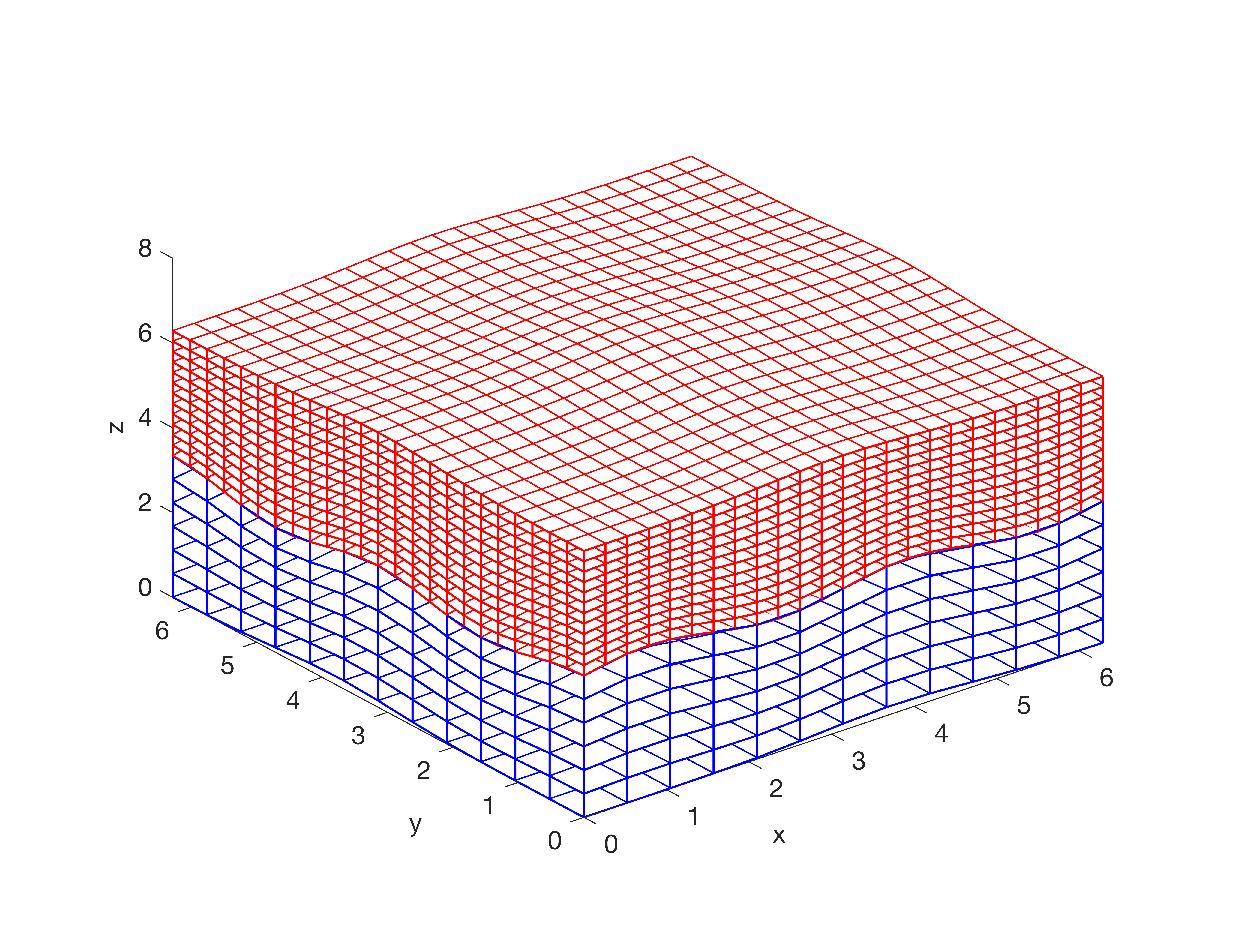
\includegraphics[width=0.6\textwidth,trim={0.4cm 0.7cm 0.8cm 1.4cm}, clip]{physical_discretization.eps}
	\caption{The sketch for the curvilinear mesh of the physical domain $\Omega$. The blue region is the spatial discretization of coarse subdomain $\Omega^c$ and the red region is the spatial discretization of the fine domain $\Omega^f$. Note that $x,y,z$ in the graph correspond to $x^{(1)}, x^{(2)}, x^{(3)}$ respectively. 
	 }\label{physical_discretization}
\end{figure}

In this section, we discretize the elastic wave equations (\ref{elastic_curvi}) and  (\ref{elastic_curvi_f}) with mesh refinement interface $\Gamma$. Without loss of generality, we assume the ratio of mesh sizes in the reference domains is $1:2$, that is the mesh sizes satisfy
\[h_1(n_1^h-1) = 1, \ \ \ h_2(n_2^h-1) = 1, \ \ \ h_3(n_3^h-1) = 1,\]
and
\[2h_1(n_1^{2h}-1) = 1, \ \ \ 2h_2(n_2^{2h}-1) = 1, \ \ \ 2h_3(n_3^{2h}-1) = 1,\]
respectively. Other ratios can be treated analogously. Figure \ref{physical_discretization} gives an illustration of the discretization of a physical domain. This is an ideal mesh if the wave speed in $\Omega^f$ is half of the wave speed in $\Omega^c$.

In seismic wave simulation, far-field boundary conditions are often imposed in the $x^{(1)}$ and $x^{(2)}$ directions. Here, our focus is on the numerical treatment of the interface conditions (\ref{interface_cond}). We assume periodic boundary conditions in $x^{(1)}$ and $x^{(2)}$, and ignore the boundaries in $x^{(3)}$. In Figure \ref{section_discretization}, we fix $x^{(2)} = 0$ and present the $x^{(1)}$-$x^{(3)}$ section of the domain $\Omega$ in both curvilinear space and parameter space.
\begin{figure}[htbp]
	\centering
	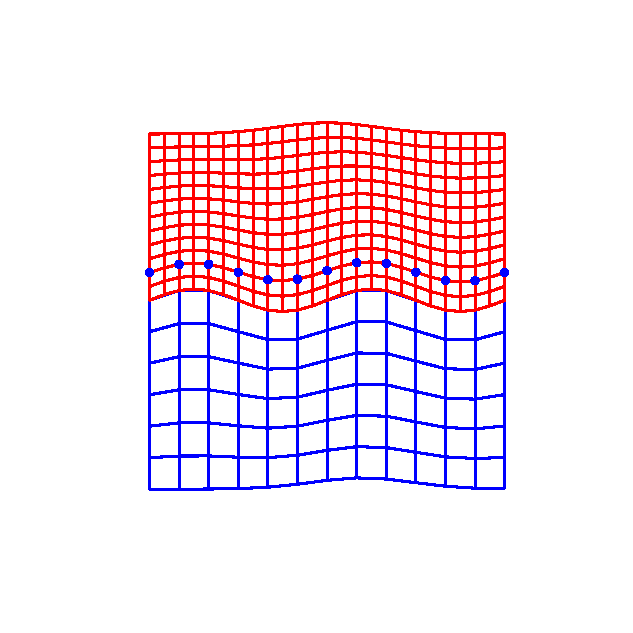
\includegraphics[width=0.45\textwidth,trim={1.0cm 2.0cm 1.0cm 1.8cm}, clip]{physical_section_discretization.eps}
	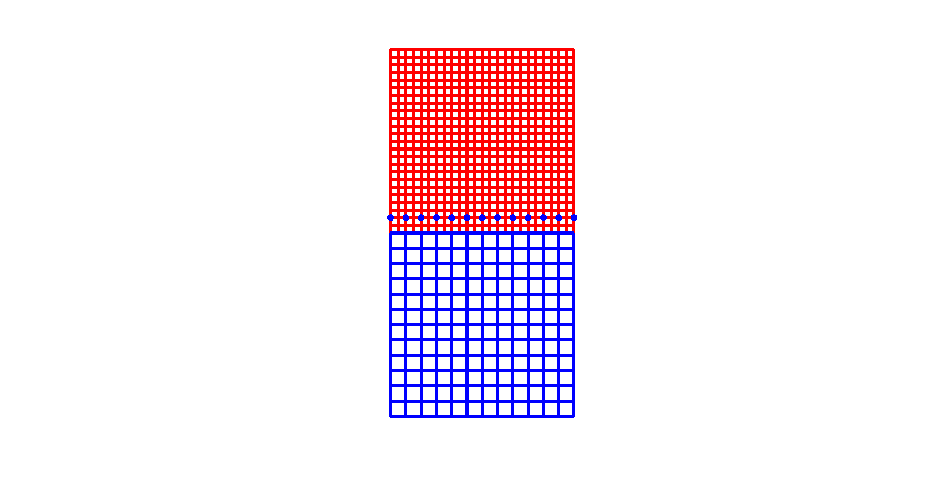
\includegraphics[width=0.45\textwidth,trim={1.0cm 2.0cm 1cm 1.8cm}, clip]{parameter_section_discretization.eps}
	\caption{The sketch of spatial discretization of $x^{(1)}$-$x^{(3)}$ section with $x^{(2)} = 0$. From the left to the right are for physical domain and parameter space, respectively. The blue dots are the ghost points for the coarse domain $\Omega^c$.}\label{section_discretization}
\end{figure}
 To condense notations, we introduce the multi-index notations
\[{\bf i} = (i,j,k),\ \ {\bf r}_{\bf i} = (r^{(1)}_i,r^{(2)}_j,r^{(3)}_k),\ \ {\bf x}_{\bf i} = (x^{(1)}_i,x^{(2)}_j,x^{(3)}_k).\]
 Note that for ${\bf x}_{\bf i}\in\Omega^f$, we have ${\bf x}_{\bf i} = {\bf X}^f({\bf r}_{\bf i})$, $i\in[1,n_1^h]$, $j\in[1,n_2^h]$, $k\in[1,n_3^h]$; for ${\bf x}_{\bf i}\in\Omega^c$, we have ${\bf x}_{\bf i} = {\bf X}^c({\bf r}_{\bf i})$, $i\in[1,n_1^{2h}]$, $j\in[1,n_2^{2h}]$, $k\in[1,n_3^{2h}]$; for ${\bf x}_{\bf i} \in \Gamma\cap\Omega^c$, we have ${\bf x}_{\bf i} = {\bf X}^c({\bf r}_{\bf i})$, $i\in[1,n_1^{2h}]$, $j\in[1,n_2^{2h}]$, $k = n_3^{2h}$; for ${\bf x}_{\bf i} \in \Gamma\cap\Omega^f$, we have ${\bf x}_{\bf i} = {\bf X}^f({\bf r}_{\bf i})$, $i\in[1,n_1^h]$, $j\in[1,n_2^h]$, $k = 1$; for ${\bf x}_{\bf i}\in \Omega \setminus \Omega^c := \overline{\Gamma}$, we have ${\bf x}_{\bf i} = {\bf X}^f({\bf r}_{\bf i})$, $i\in[1,n_1^h]$, $j\in[1,n_2^h]$, $k\in[2,n_3^h]$. %We want to mention that we have abused the symbol $\bar{\Gamma}$ a little bit to only contain the grid points in $\Omega^f$ but not in $\Omega^c$.
Now, denote the grid functions in $\Omega^f$ and $\Omega^c$ by
\[{\bf f} = ({\bf f}^1, {\bf f}^2, {\bf f}^3)^T\ \ \ \ \mbox{and}\ \ \ \  {\bf c} = ({\bf c}^1, {\bf c}^2, {\bf c}^3)^T,\]
respectively. Here, 
\[{\bf f}^l\approx F_l({\bf r}), \ \ {\bf X}^f({\bf r})\in\Omega^f,\ \ l=1,2,3 ,\]
and
\[{\bf c}^l \approx C_l({\bf r}),\ \ {\bf X}^c({\bf r})\in\Omega^c, \ \ l = 1,2,3.\]
Furthermore, we define ${\bf f}_{\Gamma}$ as the fine grid function for ${\bf X}^f({{\bf r}})\in\Gamma$, ${\bf c}_{\Gamma}$ as the coarse grid function for ${\bf X}^c({{\bf r}})\in\Gamma$ and ${\bf f}_{\overline{\Gamma}}$ as the fine grid function for ${\bf X}^f({{\bf r}})\in\overline{\Gamma}$. Particularly, we define $\wt{\bf c} = (\wt{\bf c}^1,\wt{\bf c}^2,\wt{\bf c}^3)^T$ as the coarse grid function which contains both grids in $\Omega^c$ and ghost points outside $\Omega^c$ with $i\in[1,n_1^{2h}], j\in[1,n_2^{2h}], k\in[0,n_3^{2h}+1]$. Then we approximate the elastic wave equation (\ref{elastic_curvi}) in $\Omega^c$ by
\begin{equation}\label{elastic_semi_c}
{\varrho}^{2h} {\bf c}_{tt} =( \mathcal{ J}^{2h})^{-1}\left(\sum_{l=1}^2\mathcal{G}_l^{2h}({N}_{ll}^{2h}){\bf c}+\wt{\mathcal{G}}_3^{2h}({N}_{33}^{2h}){\wt{\bf c}}+\sum_{l=1}^3\sum_{m=1,m\neq l}^3\mathcal{D}_l^{2h}(\mathcal{N}_{lm}^{2h}\mathcal{D}_m^{2h}{\bf c})\right) := \wt{\mathcal{L}}^{2h} {\wt {\bf c}},
\end{equation}
where 
\begin{align}\label{rho_j}
\varrho^{2h} = \left(\begin{array}{ccc}
{\bm \rho}^{2h}& ~  & ~ \\
~ & {\bm \rho}^{2h} & ~ \\
~ &~  &{\bm \rho}^{2h}\end{array}\right),\ \ \ \mathcal{J}^{2h} = \left(\begin{array}{ccc}
{\bf J}^{2h}& ~  & ~ \\
~ & {\bf J}^{2h} & ~ \\
~ &~  &{\bf J}^{2h}\end{array}\right)
\end{align}
with both ${\bm \rho}^{2h}$ and ${\bf J}^{2h}$ are diagonal matrices of size  $n_1^{2h}n_2^{2h}n_3^{2h}\times n_1^{2h}n_2^{2h}n_3^{2h}$. The diagonal entries of ${\bm \rho}^{2h}$ and ${\bf J}^{2h}$ are values of density function $\rho^c$ and Jacobian of transformation $J^c$ on the grids in $\Omega^c$, respectively.
The operators $\mathcal{G}_l^{2h}({N}_{ll}^{2h})$, $l=1,2$ are defined as
\begin{align*}\label{g1122}
\mathcal{G}^{2h}_l({N}_{ll}^{2h}) = \left(\begin{array}{ccc}
Q_l^{2h}(N_{ll}^{2h}(1,1)) & Q_l^{2h}(N_{ll}^{2h}(1,2))  & Q_l^{2h}(N_{ll}^{2h}(1,3)) \\
Q_l^{2h}(N_{ll}^{2h}(2,1)) & Q_l^{2h}(N_{ll}^{2h}(2,2))  & Q_l^{2h}(N_{ll}^{2h}(2,3)) \\
Q_l^{2h}(N_{ll}^{2h}(3,1)) & Q_l^{2h}(N_{ll}^{2h}(3,2))  & Q_l^{2h}(N_{ll}^{2h}(3,3)) \end{array}\right),
\end{align*}
where $Q_l^{2h}(N_{ll}^{2h}(i,j))$, $i,j = 1,2,3$, are $n_1^{2h}n_2^{2h}n_3^{2h}\times n_1^{2h}n_2^{2h}n_3^{2h}$ matrices with the central difference stencils in direction $r^{(l)}$ for second derivative with variable coefficient. Here, we also use a matlab notation $N_{ll}^{2h}(i,j)$ to represent the $i'$th row and $j'$th column of matrix $N_{ll}^{2h}$. Note that for each grid point, $N_{ll}^{2h}$ is a $3\times3$ matrix and its values are $N_{ll}^c$ evaluated at the grid points. As for $\wt{\mathcal{G}}_3^{2h}({N}_{33}^{2h})$, it has a structure
\[ \wt{\mathcal{G}}^{2h}_3({N}_{33}^{2h}) = \left(\begin{array}{ccc}
\wt{G}_3^{2h}(N_{33}^{2h}(1,1)) & \wt{G}_3^{2h}(N_{33}^{2h}(1,2))  & \wt{G}_3^{2h}(N_{33}^{2h}(1,3)) \\
\wt{G}_3^{2h}(N_{33}^{2h}(2,1)) & \wt{G}_3^{2h}(N_{33}^{2h}(2,2))  & \wt{G}_3^{2h}(N_{33}^{2h}(2,3)) \\
\wt{G}_3^{2h}(N_{33}^{2h}(3,1)) & \wt{G}_3^{2h}(N_{33}^{2h}(3,2))  & \wt{G}_3^{2h}(N_{33}^{2h}(3,3)) \end{array}\right),\]
where $\wt{G}_3^{2h}(N_{33}^{2h}(i,j))$, $i,j = 1,2,3$, are $n_1^{2h}n_2^{2h}n_3^{2h}\times n_1^{2h}n_2^{2h}(n_3^{2h}+2)$ matrices which are defined as in (\ref{sbp_2nd_1}) for direction $r^{(3)}$. 

Now, let's look at the terms $\mathcal{D}_l^{2h}(\mathcal{N}_{lm}^{2h}\mathcal{D}_m^{2h})$, $l = 1,2,3, m = 1,2,3, l\neq m$. We first explain the cases with $l = 1,2$ and $m = 1,2$ by using $\mathcal{D}_1^{2h}(\mathcal{N}_{12}^{2h}\mathcal{D}_2^{2h})$ as an example. The other cases are analogous. We have 
\begin{equation}\label{D12}
\mathcal{D}_1^{2h} = {\bf I}\otimes D_1^{2h} \otimes {\bf I}_2 \otimes {\bf I}_3,\ \ \ \mathcal{D}_2^{2h} ={\bf I}\otimes {\bf I}_1\otimes D_2^{2h}\otimes {\bf I}_3,
\end{equation}
where ${\bf I}$ is a $3\times3$ identity matrix, ${\bf I}_l$, $l = 1,2,3$ are $n_l^{2h}\times n_l^{2h}$ identity matrices, $D_1^{2h}$ is a $n_1^{2h}\times n_1^{2h}$ matrix with central difference stencil for first order derivative in direction $r^{(1)}$, $D_2^{2h}$ is a matrix of size $n_2^{2h}\times n_2^{2h}$ with central difference operator for first order derivative in direction $r^{(2)}$ as stencil, $\mathcal{N}_{12}^{2h}$ is a $3n_1^{2h}n_2^{2h}n_3^{2h}\times3n_1^{2h}n_2^{2h}n_3^{2h}$ matrix with a structure
\begin{align}\label{N12}
\mathcal{N}_{12}^{2h}= \left(\begin{array}{ccc}
\mathscr{N}_{12}^{2h,11}&\mathscr{N}_{12}^{2h,12}& \mathscr{N}_{12}^{2h,13}\\
\mathscr{N}_{12}^{2h,21} & \mathscr{N}_{12}^{2h,22} & \mathscr{N}_{12}^{2h,23} \\
\mathscr{N}_{12}^{2h,31}&\mathscr{N}_{12}^{2h,32}&  \mathscr{N}_{12}^{2h,33}\\ \end{array}\right),
\end{align}
where $\mathscr{N}_{12}^{2h,ij}$, $i,j = 1,2,3$ are diagonal matrices of size $n_1^{2h}n_2^{2h}n_3^{2h}\times n_1^{2h}n_2^{2h}n_3^{2h}$ with the diagonal values to be $N_{12}^{c}(i,j)$ evaluated at the coarse grid points, i.e., $N_{12}^{2h}(i,j)$. 

Then, let's look at the terms with either $l = 3$ or $m = 3$, we use $\mathcal{D}_1^{2h}(\mathcal{N}_{13}^{2h}\mathcal{D}_3^{2h})$ as an example and the other cases are similar,
\begin{equation}\label{D13}
\mathcal{D}_1^{2h} = {\bf I}\otimes D_1^{2h} \otimes {\bf I}_2 \otimes {\bf I}_3,\ \ \ \mathcal{D}_3^{2h} ={\bf I}\otimes {\bf I}_1\otimes {\bf I}_2\otimes D_3^{2h},
\end{equation}
where $\mathcal{D}_1^{2h}$ is defined in (\ref{D12}) and $D_3^{2h}$ is a matrix of size $n_3^{2h}\times n_3^{2h}$ defined in (\ref{first_sbp}) for direction $r^{(3)}$, $\mathcal{N}_{13}^{2h}$ has a similar definition as $\mathcal{N}_{12}^{2h}$ in (\ref{N12}).

Next, we approximate the elastic wave equation (\ref{elastic_curvi_f}) for the fine grids. We first consider all fine grid points not at the interface, and have the semi-discretization
\begin{equation}\label{elastic_semi_f}
\varrho^h_{\overline{\Gamma}} ({\bf f}_{\overline{\Gamma}})_{tt} =
( \mathcal{ J}_{\overline{\Gamma}}^{h})^{-1}\left(\sum_{l=1}^3\Big(\big(\mathcal{G}_l^{h}({N}_{ll}^h){\bf f}\big)\Big|_{\overline{\Gamma}}+\sum_{m=1,m\neq l}^3\big(\mathcal{D}_l^{h}(\mathcal{N}_{lm}^{h}\mathcal{D}_m^{h}{\bf f})\big)\Big|_{\overline{\Gamma}}\Big)\right) := \mathcal{L}^h{\bf f}\Big|_{\overline{\Gamma}},
\end{equation}
where ${\varrho}^{h}_{\overline{\Gamma}}$ and ${\mathcal{J}}^{h}_{\overline{\Gamma}}$ are $3n_1^hn_2^h(n_3^h-1)\times 3n_1^hn_2^h(n_3^h-1)$ diagonal matrices, which have similar definitions as in (\ref{rho_j}), but correspond to the grids in $\overline{\Gamma}$. In addition, the terms $\mathcal{G}_l^h({N}_{ll}^h), l = 1,2$ and $\mathcal{D}_l^h(\mathcal{N}_{lm}^h\mathcal{D}_m^h), l=1,2,3,m=1,2,3,l\neq m$ in (\ref{elastic_semi_f}) have similar definitions as in (\ref{elastic_semi_c}) but corresponds to the grids in the fine domain $\Omega^f$. And $\mathcal{G}_3^h({N}_{33}^h)$ is defined as
\[ \mathcal{G}^{h}_3({N}_{33}^h) = \left(\begin{array}{ccc}
G_3^{h}(N_{33}^{h}(1,1)) & G_3^{h}(N_{33}^{h}(1,2))  & G_3^{h}(N_{33}^{h}(1,3)) \\
G_3^{h}(N_{33}^{h}(2,1)) & G_3^{h}(N_{33}^{h}(2,2))  & G_3^{h}(N_{33}^{h}(2,3)) \\
G_3^{h}(N_{33}^{h}(3,1)) & G_3^{h}(N_{33}^{h}(3,2))  & G_3^{h}(N_{33}^{h}(3,3)) \end{array}\right),\]
where ${G}_3^{h}(N_{33}^{h}(i,j))$, $i,j = 1,2,3$, are $n_1^{h}n_2^{h}n_3^{h}\times n_1^{h}n_2^{h}n_3^{h}$ matrices which are defined as in (\ref{sbp_2nd_2}) for direction $r^{(3)}$. The symbol $(\cdot)\big|_{\bar{\Gamma}}$ in (\ref{elastic_semi_f}) corresponds to the data in $\bar{\Gamma}$.

For the approximation on the interface $\Gamma$, we obtain the numerical solution by injection using a scaled interpolation operator
\begin{equation}\label{continuous_sol}
{\bf f}_{\Gamma} = \wt{\mathcal{P}}({\bf c}_{\Gamma}),
\end{equation}
which imposes the continuity of the solution at the interface $\Gamma$. 

For energy stability, the operator $ \wt{\mathcal{P}}$ must be in a specific form 
\[\wt{\mathcal{P}} = (\mathcal{J}^h_\Gamma \bm{\Lambda}^h)^{-\frac{1}{2}}\mathcal{P}(\mathcal{J}^{2h}_\Gamma \bm{\Lambda}^{2h})^{\frac{1}{2}}.\]
Here, both  $\mathcal{P}$ and $\bm{\Lambda}^{2h}$ are $3n_1^{2h}n_2^{2h}n_3^{2h}\times 3n_1^{2h}n_2^{2h}n_3^{2h}$ matrices and the size of $\bm{\Lambda}^{h}$ is $3n_1^{h}n_2^{h}n_3^{h}\times 3n_1^{h}n_2^{h}n_3^{h}$. They have the following structures
\begin{align*}\label{iandr}
\mathcal{P} = \left(\begin{array}{ccc}
{\bf P}& ~  & ~ \\
~ & {\bf P} & ~ \\
~ &~  &{\bf P}\end{array}\right), \ \ \ 
\bm{\Lambda}^h = \left(\begin{array}{ccc}
\Lambda^h& ~  & ~ \\
~ & \Lambda^h & ~ \\
~ &~  &\Lambda^h\end{array}\right), \ \ \ \bm{\Lambda}^{2h} = \left(\begin{array}{ccc}
\Lambda^{2h}& ~  & ~ \\
~ & \Lambda^{2h} & ~ \\
~ &~  &\Lambda^{2h}\end{array}\right).
\end{align*}
The matrix $\bf P$ is of size $n_1^{2h}n_2^{2h}n_3^{2h}\times n_1^{2h}n_2^{2h}n_3^{2h}$. Since the mesh refinement ratio is $1:2$, the stencils of the fourth order accurate interpolation operator ${\bf P}$ in two dimensions have four cases, see the illustration in  Figure \ref{interpolation}. 
The matrix $\Lambda^{h}$ is a $n_1^{h}n_2^{h}n_3^{h}\times n_1^{h}n_2^{h}n_3^{h}$ diagonal matrix and its diagonal values are $|\nabla_x R^{f,(3)}|$ evaluated at the fine grid points at interface $\Gamma$. Similarly, $\Lambda^{2h}$ is a $n_1^{2h}n_2^{2h}n_3^{2h}\times n_1^{2h}n_2^{2h}n_3^{2h}$ diagonal matrix with diagonal values  $|\nabla_x R^{c,(3)}|$ evaluated at the coarse grid points at interface $\Gamma$.

We note that \eqref{continuous_sol} is equivalent to the more complicated form
\begin{equation}\label{elastic_semi_f_i}
{\varrho}^h_\Gamma ({\bf f}_\Gamma)_{tt} =
( {\mathcal{ J}}^{h}_\Gamma)^{-1}\left(\sum_{l=1}^3\Big(\big(\mathcal{G}_l^{h}({N}_{ll}^h){\bf f}\big)\Big|_\Gamma+\sum_{m=1,m\neq l}^3\big(\mathcal{D}_l^{h}(\mathcal{N}_{lm}^{h}\mathcal{D}_m^{h}{\bf f})\big)\Big|_\Gamma\Big) \right) + {\bm \eta} := \mathcal{L}^h{\bf f}\Big|_\Gamma + {\bm \eta},
\end{equation}
with 
\begin{equation}\label{eta}
{\bm \eta} = {\varrho}^h_{\Gamma}\wt{\mathcal{P}}\left(\big(({ \varrho}^{2h})^{-1}\wt{\mathcal{L}}^{2h} \wt{{\bf c}}\big)\Big|_{\Gamma}\right) - \mathcal{L}^{h}{\bf f}\Big|_{\Gamma}.
\end{equation}
Here, ${\varrho}^{h}_{\Gamma}$ and ${\mathcal{ J}}^{h}_{\Gamma}$ are $3n_1^hn_2^h\times 3n_1^hn_2^h$ diagonal matrices with similar definitions as in (\ref{rho_j}) with fine grids at $\Gamma$. The size of the column vector $\big(({\varrho}^{2h})^{-1}\wt{L}^{2h} \wt{{\bf c}}\big)\big|_{\Gamma}$ is $3n_1^{2h} n_2^{2h}$. 

 We note that $\bm \eta$ in (\ref{eta}) is approximately zero with a second order truncation error, which is of the same order as the boundary stencil of the SBP operator. Therefore, it does not affect the overall accuracy of the semi-discretization. 

For the simplicity of analysis, we introduce a general notation for the schemes (\ref{elastic_semi_f}) and (\ref{elastic_semi_f_i}) in the fine domain $\Omega^f$,
\begin{align}\label{fine_scheme}
{\varrho}^h{\bf f}_{tt} = \hat{\mathcal{L}}^h{\bf f} = \left\{
\begin{aligned}
&\mathcal{L}^h{\bf f}\big|_\Gamma +{\bm \eta}, \\
&\mathcal{L}^h{\bf f}\big|_{\overline{\Gamma}}.
\end{aligned}
\right.
\end{align}
In computer implementation, we use \eqref{continuous_sol} to obtain the solution on the interface of the fine domain. The reason of introducing    \eqref{elastic_semi_f_i} is that it will be helpful in the energy analysis in Sec.\ref{sec_energy}.

The following condition imposes continuity of traction at the interface,
\begin{equation}\label{continuous_traction}
(\bm{\Lambda}^{2h}{\mathcal J}_{\Gamma}^{2h})^{-1}\big(\wt{\mathcal{A}}_3^{2h}\wt{\bf c}\big)\big|_\Gamma
= \wt{\mathcal{R}}\left((\bm{\Lambda}^{h}{\mathcal J}^h_{\Gamma})^{-1}((\mathcal{A}_3^h{\bf f})\big|_\Gamma-h_3\omega_1{\mathcal J}^h{\bm \eta})\right),
\end{equation}
where we have used the notations
\begin{equation}\label{hatAf}
(\mathcal{A}_3^h{\bf f})\big|_\Gamma = (\mathcal{N}_{31}^{h}\mathcal{D}^h_1{\bf f})\big|_\Gamma + (\mathcal{N}_{32}^h\mathcal{D}^h_2{\bf f})\big|_\Gamma + (\mathcal{N}_{33}^h\mathscr{D}_3^h{\bf f})\big|_\Gamma,
\end{equation}
and
\begin{equation}\label{hatAc}
(\wt{\mathcal{A}}_3^{2h}\wt{\bf c})\big|_\Gamma = (\mathcal{N}_{31}^{2h}\mathcal{D}^{2h}_1{\bf c})\big|_\Gamma + (\mathcal{N}_{32}^{2h}\mathcal{D}^{2h}_2{\bf c})\big|_\Gamma + (\mathcal{N}_{33}^{2h}\wt{\mathscr D}^{2h}_3\wt{\bf c})\big|_\Gamma.
\end{equation}
Here, $\omega_1$ is the first entry in the scalar product (\ref{inner_product}), $\wt{\mathscr{D}}_3^{2h}$ is defined as
\[\wt{\mathscr{D}}_3^{2h} = {\bf I}\otimes {\bf I}_1 \otimes {\bf I}_2 \otimes \wt{\mathfrak{D}}_3^{2h},\]
where ${\bf I}$ is a $3\times3$ identity matrix, ${\bf I}_l$, $l = 1,2$ are $n_l^{2h}\times n_l^{2h}$ identity matrices, $\wt{\mathfrak{D}}_3^{2h}$ is a $n_3^{2h}\times (n_3^{2h}+2)$ matrix defined in (\ref{sbp_1st_1}) for direction $r^{(3)}$. In $\wt{\mathfrak{D}}_3^{2h}$, only the last row of  has $5$ non-zeros and the rest of the elements are zeros. As for $\mathscr{D}_3^{h}$, it is defined as
\[\mathscr{D}_3^{h} = {\bf I}\otimes {\bf I}_1 \otimes {\bf I}_2 \otimes {\mathfrak{D}}_3^{h},\]
where ${\bf I}$ is a $3\times3$ identity matrix, ${\bf I}_l$, $l = 1,2$ are $n_l^{h}\times n_l^{h}$ identity matrices, $\mathfrak{D}_3^{h}$ is a $n_3^{h}\times n_3^{h}$ matrix defined in (\ref{sbp_1st_2}) for direction $r^{(3)}$. The sparse matrix $\mathfrak{D}_3^{h}$ has $5$ nonzeros in the first row, and zeros elsewhere. The condition \eqref{continuous_traction} determines the ghost point values in the coarse domain. 

The scaled restriction operator $\wt{\mathcal{R}} $ has the structure 
 \[\wt{\mathcal{R}} =  (\mathcal{J}^{2h}_\Gamma \bm{\Lambda}^{2h})^{-\frac{1}{2}}\mathcal{R}(\mathcal{J}^{h}_\Gamma \bm{\Lambda}^h)^{\frac{1}{2}},\]
 where
\begin{align*}
\ \ \mathcal{R} = \left(\begin{array}{ccc}
{\bf R}& ~  & ~ \\
~ & {\bf R} & ~ \\
~ &~  &{\bf R}\end{array}\right),
\end{align*}
and ${\bf R}$ is determined by the compatibility condition ${\bf R}=\frac{1}{4}{\bf P}^T$ and its stencil is presented in Figure \ref{restriction}. As will be seen later, the compatibility condition as well as the scaling of the interpolation and restrictions are essential for energy stability \cite{Lundquist2018}.

\begin{figure}%[htbp]
	\centering
	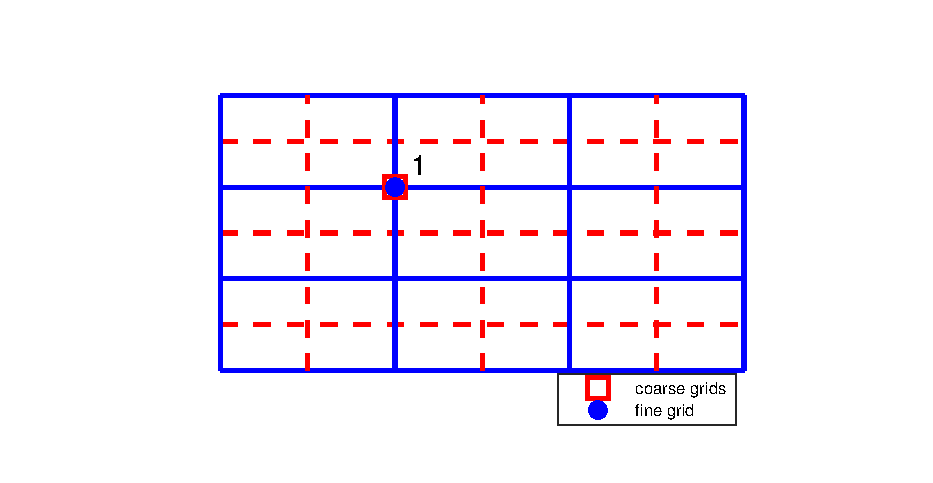
\includegraphics[width=0.24\textwidth,trim={1.8cm 0.8cm 1.4cm 1.2cm}, clip]{interpolation1.eps}
	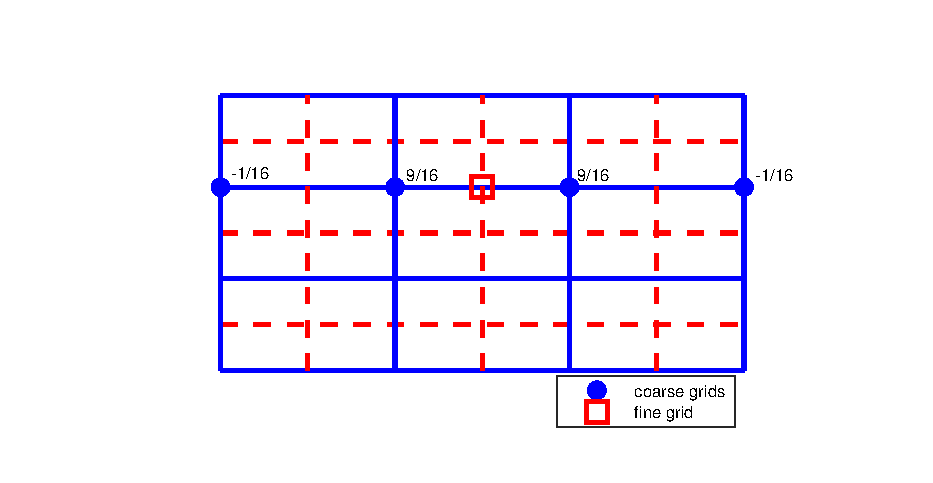
\includegraphics[width=0.24\textwidth,trim={1.8cm 0.8cm 1.4cm 1.2cm}, clip]{interpolation2.eps}
	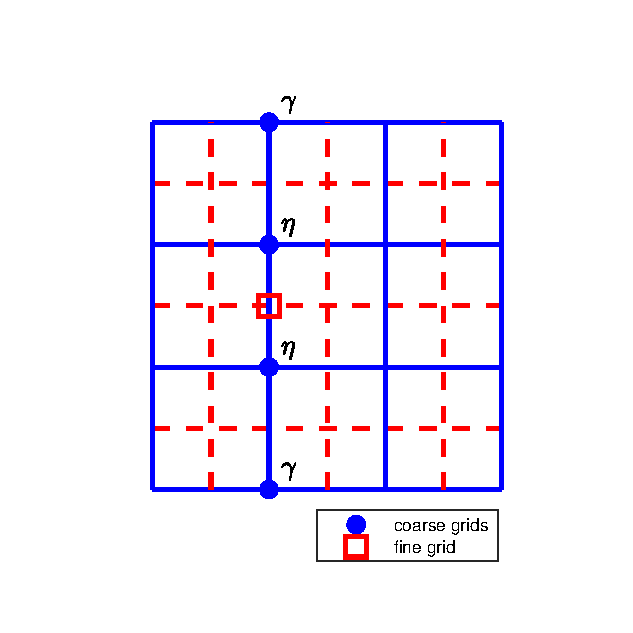
\includegraphics[width=0.24\textwidth,trim={1.8cm 0.8cm 1.4cm 1.2cm}, clip]{interpolation3.eps}
	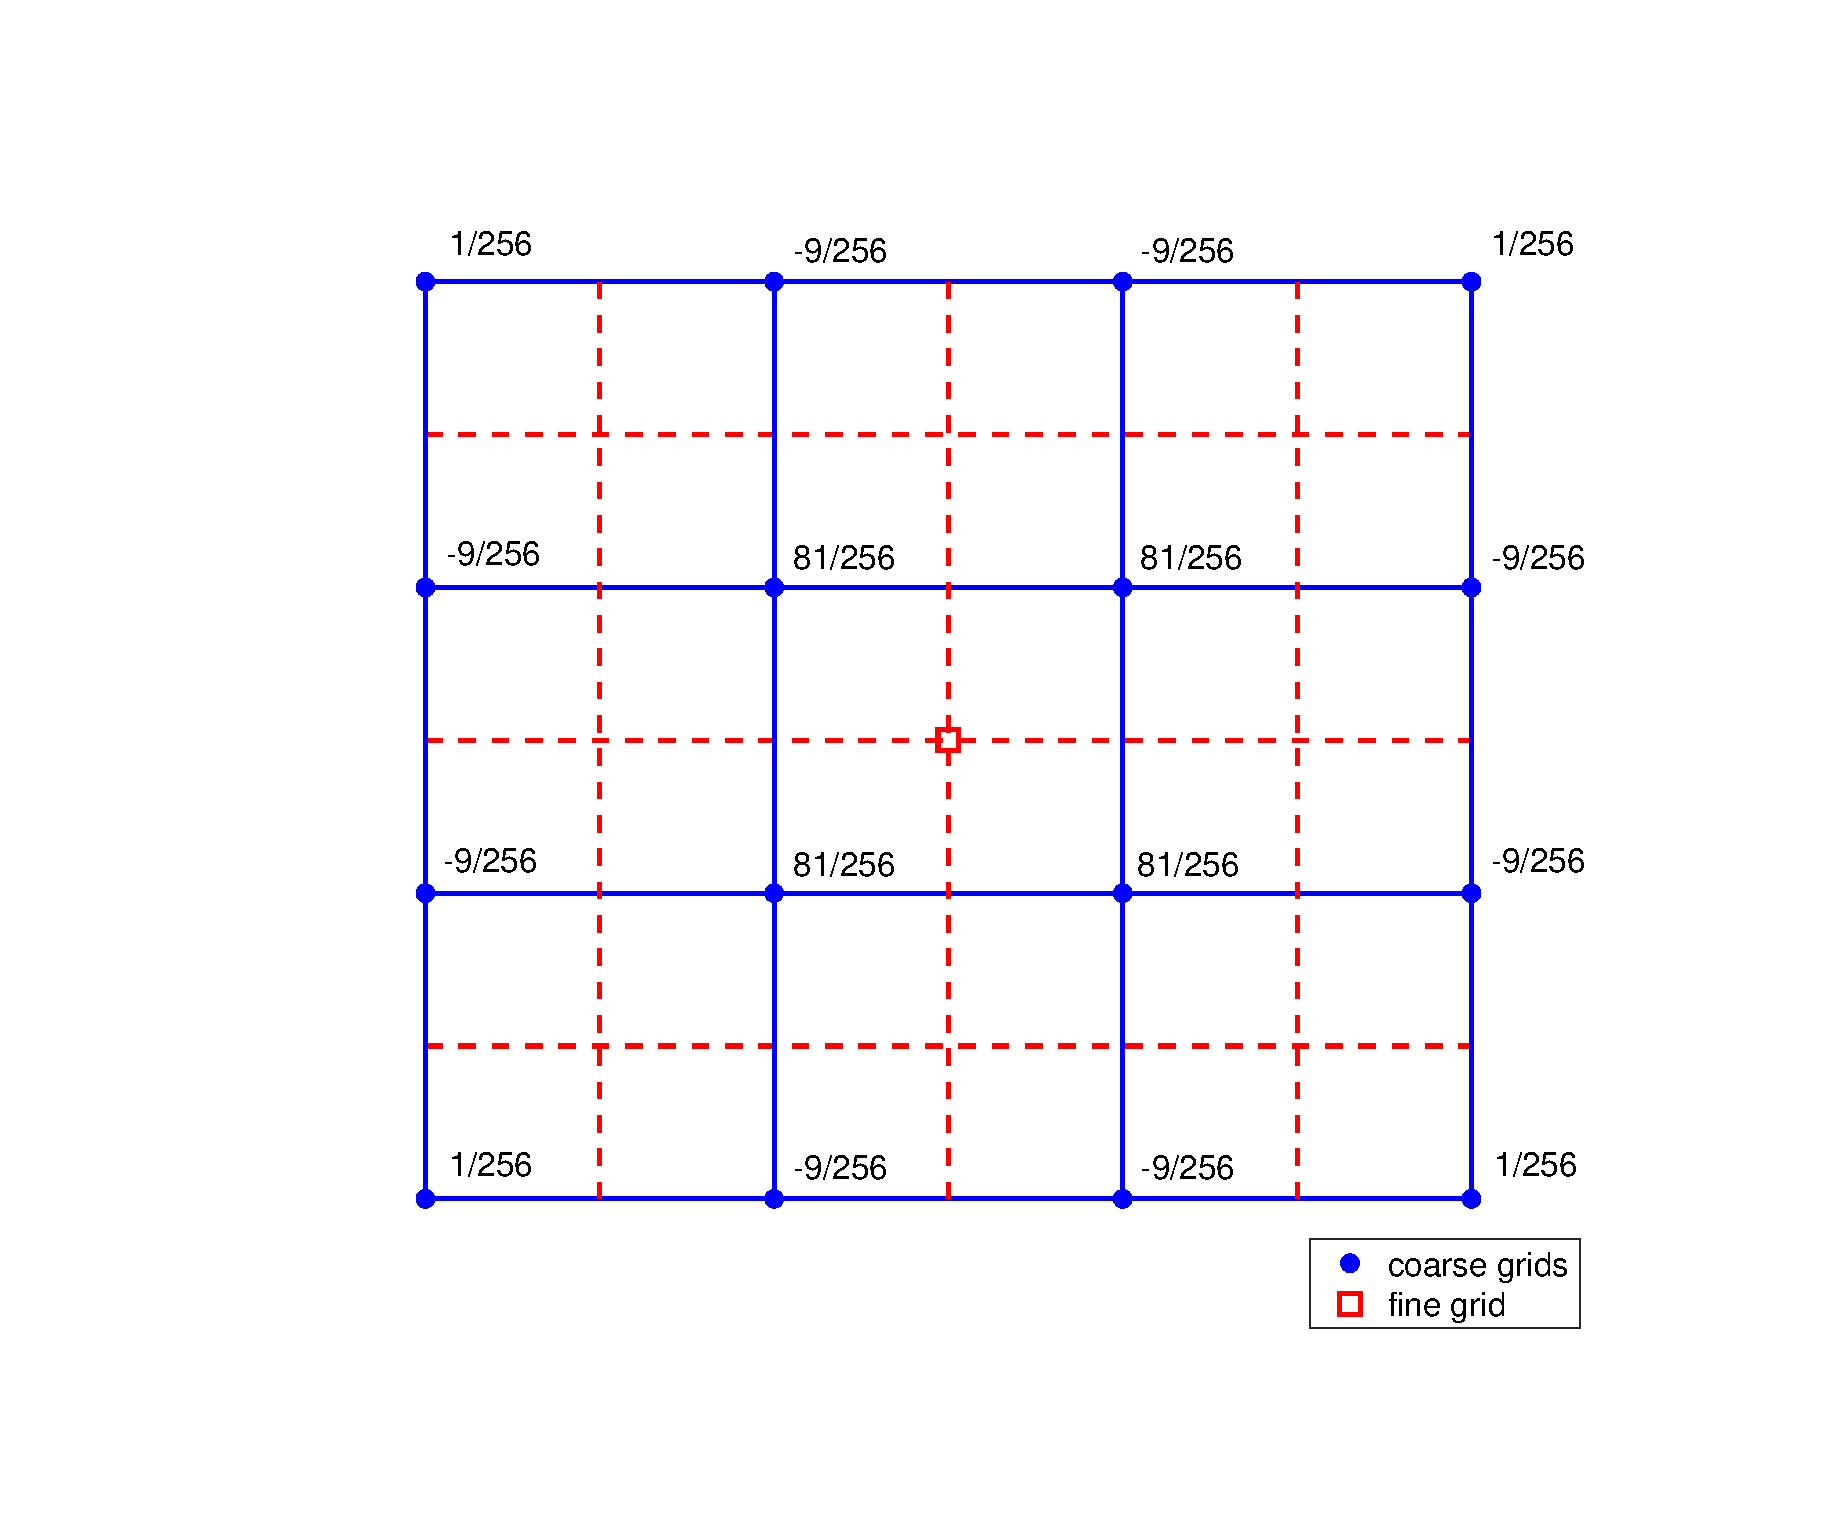
\includegraphics[width=0.24\textwidth,trim={1.8cm 0.8cm 1.4cm 1.2cm}, clip]{interpolation4.eps}
	\caption{The sketch for the stencils of fourth order interpolation operator ${\bf P}$ in two dimensions with parameters $\gamma = -\frac{1}{16}$, $\eta = \frac{9}{16}$, $\mu = 1$, $\alpha = \frac{1}{256}$, $\beta = -\frac{9}{256}$ and $\theta = \frac{81}{256}$. }\label{interpolation}
\end{figure}
\begin{figure}[htbp]
	\centering
	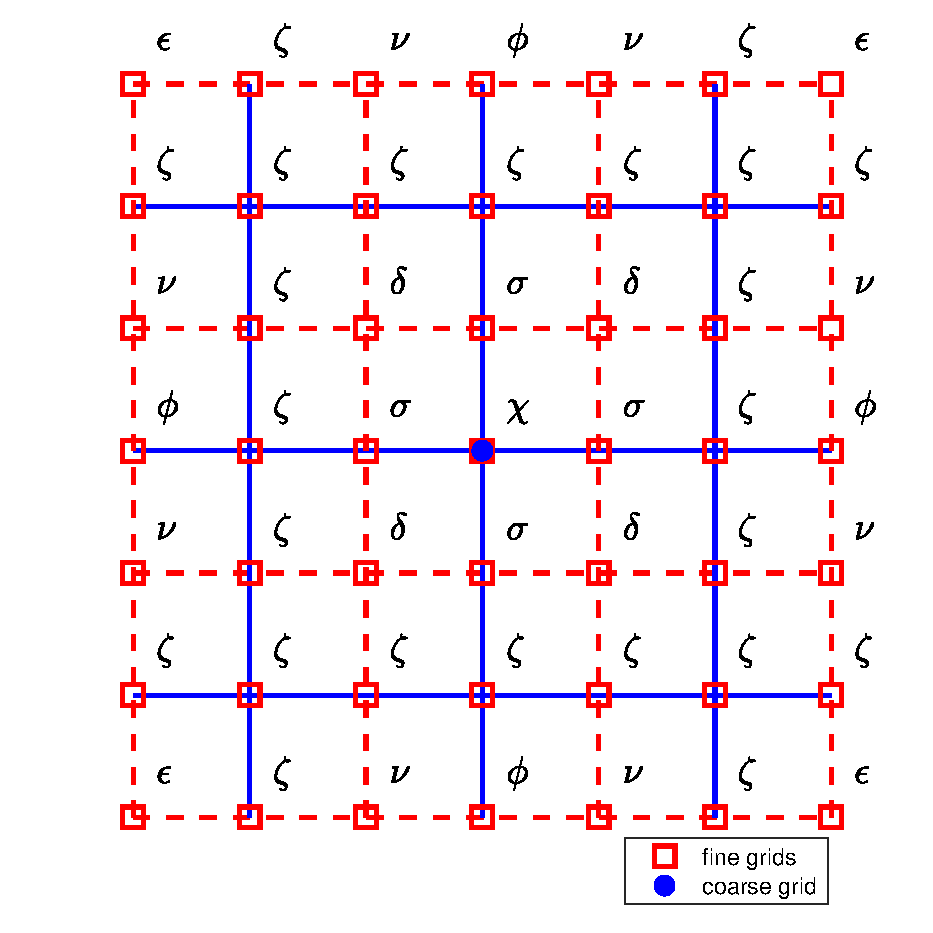
\includegraphics[width=0.6\textwidth]{restriction.eps}
	\caption{The sketch for the stencil of fourth order restriction operator ${\bf R}$ in two dimensions with parameters $\epsilon = \frac{1}{1024}$, $\nu = -\frac{9}{1024}$, $\phi = -\frac{16}{1024}$, $\delta = \frac{81}{1024}$, $\sigma = \frac{144}{1024}$, $\chi = \frac{256}{1024}$ and $\zeta = 0$.}\label{restriction}
\end{figure}






%!TEX root = SISC_elastic_3d.tex
\subsection{Energy estimate}\label{sec_energy}
In this section, we derive an energy estimate for the semi-discretization (\ref{elastic_semi_c}) and (\ref{fine_scheme}) in Sec.~\ref{semi_discrete_form}. Let ${\bf u}, {\bf v}$ be grid functions in the coarse domain $\Omega^c$ and define the three dimensional discrete scalar product in $\Omega^c$ as
\begin{equation}\label{scalar_product_inner}
({\bf v}, {\bf u})_{2h} = 8h_1h_2h_3\sum_{i=1}^{n_1^{2h}}\sum_{j=1}^{n_2^{2h}}\sum_{k=1}^{n_3^{2h}}\omega_k{J}_{i,j,k}^{c}({\bf v}_{i,j,k}\cdot {\bf u}_{i,j,k}).
\end{equation}
Similarly, define the three dimensional discrete scalar product in $\Omega^f$ as
\begin{equation}\label{scalar_product_inner_f}
({\bf v}, {\bf u})_{h} = h_1h_2h_3\sum_{i=1}^{n_1^{h}}\sum_{j=1}^{n_2^{h}}\sum_{k=1}^{n_3^{h}}\omega_k{J}_{i,j,k}^{f}({\bf v}_{i,j,k}\cdot {\bf u}_{i,j,k}),
\end{equation}
where $\bf u$ and $\bf v$ are grid functions in the fine domain $\Omega^f$. Now, we are ready to state the energy estimate of the proposed schemes in Section \ref{semi_discrete_form}. 
\begin{theorem}\label{thm1}
	The semi-discretization (\ref{elastic_semi_c}) and (\ref{fine_scheme}) is energy stable if the interface conditions \eqref{continuous_sol} and \eqref{continuous_traction} are satisfied.
\end{theorem}
\begin{proof}
	Multiplying (\ref{elastic_semi_c}) by $8h_1h_2h_3\omega_kJ^{c}{\bf c}_t$ and summing over all grid points, based on \eqref{scalar_product_inner}, we have
	\begin{equation}\label{coarse_simple}
	({\bf c}_t, {\rho}^{c}{\bf c}_{tt})_{2h} = ({\bf c}_t,({J^c})^{-1}\wt{\mathcal{L}}^{2h}{\bf c})_{2h} = -\mathcal{S}_{2h}({\bf c}_t,{\bf c}) + B_{2h}({\bf c}_t,{{\bf c}}),
	\end{equation}
	where $\mathcal{S}_{2h}({\bf c}_t,{\bf c})$ is a symmetric and positive definite bilinear form given in Appendix \ref{appendix_bf}, the boundary term $B_{2h} ({\bf c}_t,{\bf c})$ is given by
	\begin{equation}\label{bounary_c1}
	B_{2h} ({\bf c}_t,{\bf c}) = 4h_1h_2\sum_{{\bf i}\in I_{\Gamma^c}}\frac{d{\bf c}_{\bf i}}{dt}\cdot (\wt{A}_3^{2h}{\bf c}_{\bf i}),
	\end{equation}
	where $\wt{A}_3^{2h} {\bf c}$ is defined in \eqref{hatAc}. Multiplying (\ref{fine_scheme}) by $h_1h_2h_3\omega_kJ^f{\bf f}_t$ and summing over all grid points, based on \eqref{scalar_product_inner_f}, we obtain
	\begin{equation}\label{fine_simple}
	({\bf f}_t, {\rho}^f{\bf f}_{tt})_h = ({\bf f}_t,({J^f})^{-1}\hat{\mathcal{L}}^h{\bf f})_h = -\mathcal{S}_{h}({\bf f}_t,{\bf f}) + B_h({\bf f}_t,{\bf f}) 
	+h_1h_2h_3\omega_1\sum_{i = 1}^{n_1^h}\sum_{j=1}^{n_2^h} \frac{d{\bf f}_{i,j,1}}{dt}\cdot{\bm \eta}_{i,j,1}.
	\end{equation}
Here, $\mathcal{S}_h$ is also a symmetric and positive definite bilinear form given in Appendix \ref{appendix_bf}. The boundary term $B_h ({\bf f}_t,{\bf f})$ has the following form
	\begin{equation}\label{boundary_f1}
	B_h ({\bf f}_t,{\bf f}) = -h_1h_2\sum_{{\bf i}\in I_{\Gamma^f}}\frac{d{\bf f}_{\bf i}}{dt}\cdot(A_3^h {\bf f}_{\bf i}),
	\end{equation}
	where $A_3^h {\bf f}$ is given in \eqref{hatAf}. Adding \eqref{coarse_simple} and \eqref{fine_simple} together, we have
	\begin{multline}\label{semi_energy_1}
	\frac{d}{dt}\big[({\bf f}_t,\rho^f {\bf f}_t)_h + \mathcal{S}_{h}({\bf f},{\bf f}) + ({\bf c}_t,\rho^{c} {\bf c}_t)_{2h} + \mathcal{S}_{2h}({\bf c},{\bf c}) \big]  = \\
	2B_{h}({\bf f}_t,{\bf f}) + 2B_{2h}({\bf c}_t,{\bf c}) + 2h_1h_2h_3\omega_1\sum_{i = 1}^{n_1^h}\sum_{j=1}^{n_2^h}\frac{d{\bf f}_{i,j,1}}{dt}\cdot{\bm \eta}_{i,j,1}.
	\end{multline}
	Substituting (\ref{boundary_f1}) and (\ref{bounary_c1}) into (\ref{semi_energy_1}) and combining the definitions of the scalar product at the interface (\ref{scalar_product_discrete_interface_c})--(\ref{scalar_product_discrete_interface_f}) and Lemma \ref{lemma1}, we get
	\begin{align*}\label{semi_energy_2}
	&\hspace{0.4cm}\frac{d}{dt}\left[({\bf f}_t,\rho^f {\bf f}_t)_{h} + \mathcal{S}_{h}({\bf f},{\bf f}) + ({\bf c}_t,\rho^{c} {\bf c}_t)_{2h} + \mathcal{S}_{2h}({\bf c},{\bf c}) \right]   \nonumber\\
	& = 2\left<{\bf f}_t,\big(({\Lambda}^{h}{J}^h_\Gamma\big)\otimes {\bf I})^{-1}(-\mathcal{A}_3^h{\bf f}+h_3\omega_1{\bm \eta})\right>_{h}+ 2\left<{\bf c}_t,\big(({\Lambda}^{2h}{J}^{2h}_\Gamma\big)\otimes{\bf I})^{-1}\wt{\mathcal{A}}_3^{2h}{\bf c}\right>_{2h} \nonumber\\
	& = 2\left<{\mathcal{P}}{\bf c}_t,\big(({\Lambda}^{h}{J}^h_\Gamma)\otimes{\bf I}\big)^{-1}(-\mathcal{A}_3^h{\bf f}+h_3\omega_1{\bm \eta})\right>_{h}+ 2\left<{\bf c}_t, \big(({\Lambda}^{2h}{J}^{2h}_\Gamma)\otimes{\bf I}\big)^{-1}\wt{\mathcal{A}}_3^{2h}{\bf c}\right>_{2h} \nonumber\\
	& = 2\left<{\bf c}_t,{\mathcal{R}}\Big(\big(({\Lambda}^{h}{J}^h_\Gamma)\otimes{\bf I}\big)^{-1}(-\mathcal{A}_3^h{\bf f}+h_3\omega_1{\bm \eta})\Big)\right>_{2h}+ 2\left<{\bf c}_t,\big(({\Lambda}^{2h}{J}^{2h}_\Gamma)\otimes{\bf I}\big)^{-1}\wt{\mathcal{A}}_3^{2h}{\bf c}\right>_{2h} = 0,
	\end{align*}
	where ${\bf I}$ is a $3\times3$ identity matrix. Note that the discrete energy for the semi-discretization \eqref{elastic_semi_c} and \eqref{fine_scheme} is gievn by $({\bf f}_t,\rho^f {\bf f}_t)_{h} + \mathcal{S}_{h}({\bf f},{\bf f}) + ({\bf c}_t,\rho^{c} {\bf c}_t)_{2h} + \mathcal{S}_{2h}({\bf c},{\bf c})$.
\end{proof}








 

%!TEX root = elastic_3d_sbp.tex
\section{The temporal discretization}
The equations are advanced in time with an explicit fourth order accurate predictor-corrector time integration method. Like all explicit time stepping methods, there is a maximum time step not exceed CFL stabilitity limit.

In \cite{petersson2015wave}, it is proved that the time step constraint by CFL condition for the Newmark scheme 
\begin{equation*}
\varrho^h\frac{{\bf f}^{n+1}-2{\bf f}^n + {\bf f}^{n-1}}{\Delta_t^2} = \hat{\mathcal{L}}^h {\bf f}^n, \ \ \ 
\varrho^{2h}\frac{{\bf c}^{n+1}-2{\bf c}^n + {\bf c}^{n-1}}{\Delta_t^2} = \wt{\mathcal{L}}^{2h} \wt{\bf c}^n, \ \ \ n = 0,1,\cdots,
\end{equation*}
which is second order with
\begin{equation*}
\frac{\Delta_t^2}{h^2}\kappa_{\text{max}}\leq C_{\text{cfl}}^2
\end{equation*}
for the elastic wave equaiton with a homogeneous material and periodic boundary conditions, provided $h_1 = h_2 = h_3 = h$. Here, 
$\kappa_{\text{max}}$ is the maximum of the eigenvalue of the matrices 
\[T_{\bf i}^{\{f,c\}} = \frac{1}{\rho^{\{f,c\}}({\bf r}_{\bf i})}\left(\begin{array}{ccc}
Tr(N_{11}^{\{f,c\}}({\bf r}_{\bf i})) &  Tr(N_{12}^{\{f,c\}}({\bf r}_{\bf i}))& Tr(N_{13}^{\{f,c\}}({\bf r}_{\bf i}))\\
Tr(N_{21}^{\{f,c\}}({\bf r}_{\bf i})) & Tr(N_{22}^{\{f,c\}}({\bf r}_{\bf i})) & Tr(N_{23}^{\{f,c\}}({\bf r}_{\bf i}))\\
Tr(N_{31}^{\{f,c\}}({\bf r}_{\bf i})) & Tr(N_{32}^{\{f,c\}}({\bf r}_{\bf i})) & Tr(N_{33}^{\{f,c\}}({\bf r}_{\bf i}))\end{array}\right), \]
where $Tr(N_{lm}^{\{f,c\}}({\bf r}_{\bf i}))$ represents the trace of $3\times3$ matrix $N_{lm}^{\{f,c\}}({\bf r}_{\bf i}),l,m = 1,2,3$. In this paper, we use the predictor-corrector strategy to obtain a fourth order time integrator. In \cite{sjogreen2012fourth}, it shows that the fourth order scheme has a somewhat larger stability limit for the time step, but the way used to approximate eigenvalues is same. We use $C_{\text{cfl}} = 1.3175$ in the numrical experiments in this paper.

%!TEX root = SISC_elastic_3d.tex
\section{Numerical Experiments}
In this section, we conduct several numerical experiments. In Section \ref{convergence_study}, we verify the order of the convergence of the proposed scheme (\ref{elastic_semi_c}), (\ref{fine_scheme}) and (\ref{continuous_sol})--(\ref{continuous_traction}). The efficiency of iterative methods which are used to solve the interface condition system (\ref{traction_gamma_pre}) and (\ref{traction_gamma_corr}) is shown in Section \ref{iterative_section}, note that the coefficient matrices in (\ref{traction_gamma_pre}) and (\ref{traction_gamma_corr}) are same. In Section \ref{gaussian_source}, we show that there is no obvious reflection at the mesh refinement interface for the proposed scheme (\ref{elastic_semi_c}), (\ref{fine_scheme}) and (\ref{continuous_sol})--(\ref{continuous_traction}) with a traction force on the top surface. Finally, the energy conservation property is shown in Section \ref{conserved_energy}.

%!TEX root = SISC_elastic_3d.tex
\subsection{Verification of convergence rate}\label{convergence_study}
We use the method of the manufactured solution to verify the theoretical convergence order of the proposed scheme. Specifically, we take the computation domain to be 
\begin{equation}\label{coarse_domain_manufactured}
\left\{
\begin{aligned}
& x^{c,1} = 2\pi r^1\\
& x^{c,2} = 2\pi r^2\\
& x^{c,3} = r^3\theta_i\big(r^1,r^2\big) + (1-r^3)\theta_b\big(r^1,r^2\big)
\end{aligned}
\right.
\end{equation}
for coarse domain $\Omega^c$. Here, $0\leq r^1, r^2, r^3\leq 1$, $\theta_i$ is the interface surface geometry,
\begin{equation}\label{iterface_geometry}
\theta_i\big(r^1,r^2\big) = \pi+0.2\sin(4\pi r^1)+0.2\cos(4\pi r^2),
\end{equation}
and 
$\theta_b$ is the bottom surface geometry,
\begin{equation}\label{bottom_geometry}
\theta_b\big(r^1,r^2\big) = 0.2\exp\left(-\frac{(r^1-0.6)^2}{0.04}\right)+0.2\exp\left(-\frac{(r^2-0.6)^2}{0.04}\right).
\end{equation}
As for the fine domian $\Omega^f$, it is chosen to be
\begin{equation}\label{fine_domain_manufactured}
\left\{
\begin{aligned}
& x^{f,1} = 2\pi r^1\\
& x^{f,2} = 2\pi r^2\\
& x^{f,3} = r^3\theta_t\big(r^1,r^2\big) + (1-r^3)\theta_i\big(r^1,r^2\big),
\end{aligned}
\right.
\end{equation}
where $0\leq r^1, r^2, r^3\leq 1$, $\theta_t$ is the top surface geometry,
\begin{equation}\label{top_geometry}
\theta_t\big(r^1,r^2\big) = 2\pi+0.2\exp\left(-\frac{(r^1-0.5)^2}{0.04}\right)+0.2\exp\left(-\frac{(r^2-0.5)^2}{0.04}\right),
\end{equation}
and $\theta_i$ is the interface geometry which is given in (\ref{iterface_geometry}). For both fine and coarse domians, let the density vary according to
\begin{equation}\label{density_function}
\rho(x^1,x^2,x^3) = 2 + \sin(x^1+0.3)\sin(x^2+0.3)\sin(x^3-0.2),
\end{equation}
and material parameters $\mu, \lambda$ satisfy
\begin{equation}\label{mu_function}
\mu(x^1,x^2,x^3) = 3 + \sin(3x^1+0.1)\sin(3x^2+0.1)\sin(x^3),
\end{equation}
and 
\begin{equation}\label{lambda_function}
\lambda(x^1,x^2,x^3)  = 21+ \cos(x^1+0.1)\cos(x^2+0.1)\sin^2(3x^3),
\end{equation}
respectively. Besides, we impose a boundary forcing on the top surface and Dirichlet boundary conditions for the other boundaries. The external forcing, top boundary forcing ${\bf g}$ and initial conditions are chosen such that ${\bf u}(\cdot,t) = (u_1(\cdot,t),u_2(\cdot,t),u_3(\cdot,t))^T$ with
\begin{align*}
u_1(\cdot,t) &= \cos(x^1+0.3)\sin(x^2+0.3)\sin(x^3+0.2)\cos(t^2),\\
u_2(\cdot,t) &= \sin(x^1+0.3)\cos(x^2+0.3)\sin(x^3+0.2)\cos(t^2),\\
u_3(\cdot,t) &= \sin(x^1+0.2)\sin(x^2+0.2)\cos(x^3+0.2)\sin(t).
\end{align*}
For example, for the boundary forcing on the top surface, we impose 
\begin{equation}\label{traction_force}
{\bf g} = (g_1,g_2,g_3)^T = \sum_{i=1}^3\left(\sum_{j = 1}^3 M_{ij}^f\frac{\partial{\bf u}}{\partial x^{(j)}}\right) n^{f,+,i}_3,
\end{equation}
where, $M_{ij}^f$ and $n^{f,+,i}_3 $ can be found in (\ref{M_definition}) and (\ref{outward_normal}) respectively.

The convergence rate is computed by
\[log\left(\frac{e_h}{e_{2h}}\right)\Bigg/log\left(\frac{1}{2}\right),\]
here, $e_h$ is the corresponding $L^2$ error.  The problem is evolved until final time $T = 0.5$. The $L^2$ error for the numerical solutions in the whole domain, $L^{f,2}$ error for the numerical solutions in the fine domain $\Omega^f$ and$L^{c,2}$ error for the numerical solutions in the coarse domain $\Omega^c$ are presented in Table \ref{convergence_rate}, note that the convergence rates are shown in the bracket of the Table \ref{convergence_rate}. We observe that the convergence rate is fourth order for all cases, though the theoretical convergence rate is second for the points near boundaries. We want to mention that a block Jacobian iterative method is used for the experiments here, and we are going to give more details about the iterative methods in the Section \ref{iterative_section}.

\begin{table}[htb]
	\begin{center}
		\begin{tabular}{|c|c c c|}
			\hline
			$2h_1 = 2h_2 = 2h_3 = 2h$   & $L^2$ & $L^{f,2}$ & $L^{c,2}$  \\
			\hline
			$2\pi/24$ &2.2227e-03 ~~~~~~~~ & 8.0442e-04 ~~~~~~~~ & 2.0720e-03 ~~~~~~~~\\
			\hline
			$2\pi/48$ &1.4142e-04 (3.97) & 5.1478e-05 (3.97) & 1.3171e-04 (3.98)\\
			\hline 
			$2\pi/96$ &8.6166e-06 (4.04) & 3.0380e-06 (4.08) & 8.0632e-06 (4.03)\\
			\hline
		\end{tabular}
	\end{center}
	\caption{Convergence rate of the fourth order SBP method}\label{convergence_rate}
\end{table} 


%!TEX root = elastic_3d_sbp.tex
\subsubsection{Iterative methods}\label{iterative_section}
In the proposed scheme (\ref{coarse_scheme})--(\ref{traction_continuous_curvi}), we need to solve a $3n_1^cn_2^c\times 3n_1^cn_2^c$ linear system at each time step twice for the continutiy of the traction force along the interface (\ref{traction_gamma_pre}) and (\ref{traction_gamma_corr}). Even ethough we can do LU factorization one time before the time loop start and reuse it at each time step, it is very expensive to do LU factorization for a large problem. Besides, consider solving real problems which are usually in large scale, we want to perform the computation on many processors on a parallel distributed memory machine, but it is not clear how to calculate the LU factorization of a matrix on many processors. 

In this paper, we propose three iterative methods: block Jacobian method, conjugate gradient method, preconditioned conjugate gradient method. We find that preconditioned conjugate gradient method is the most efficient one and conjugate gradient method needs most iteration numbers.

For the problem proposed in Section \ref{manufactured_sol}, the structure of the coefficient matrix of the linear system (\ref{traction_continuous_curvi}) is shown in Figure \ref{Mass_matrix} which is determined by the interplation operator $\mathcal{P}$ and restriction operator $\mathcal{R}$. We choose the red circles in the purple circles in Figure \ref{Mass_matrix} to be the block Jacobian matrix in block Jacobian iterative method and pre-conditioning matrix in pre-conditioned conjugate gradient iterative method. We also set a absolute error tolerance $1e-7$ for each iterative method.

\begin{table}[htbp]
	\begin{center}
		\begin{tabular}{|c|c c c|}
			\hline
			$h^c_k = 2h^f_k$   & ~~~~ CG ~~~~& Block Jacobian & Preconditioned CG  \\
			\hline
			$2\pi/24$ &37.76& 24.96& 4.07\\
			\hline
			$2\pi/48$ &38.61 & 25.38 & 2.88\\
			\hline 
			$2\pi/96$ &39.14 &25.43 & 2.55\\
			\hline
		\end{tabular}
	\end{center}
	\caption{condition number of matrices in conjugate gradient method, block Jacobian method, preconditioned conjugate gradient method}\label{condition_number}
\end{table} 
Table \ref{condition_number} shows the condition number of the original coefficient matrix, the block Jacobian matrix and the coefficient matrix after applying pre-conditioner respectively. We observe that the condition number for preconditioned conjugate gradient method is smallest which is consistent with the results for iteration number of different iterative methods : there is around $44$ iterations for conjugate gradient method, $13$ iterations for block Jacobian method and $9$ iterations for preconditioned conjugate method.

\begin{figure}[H]
	\centering
	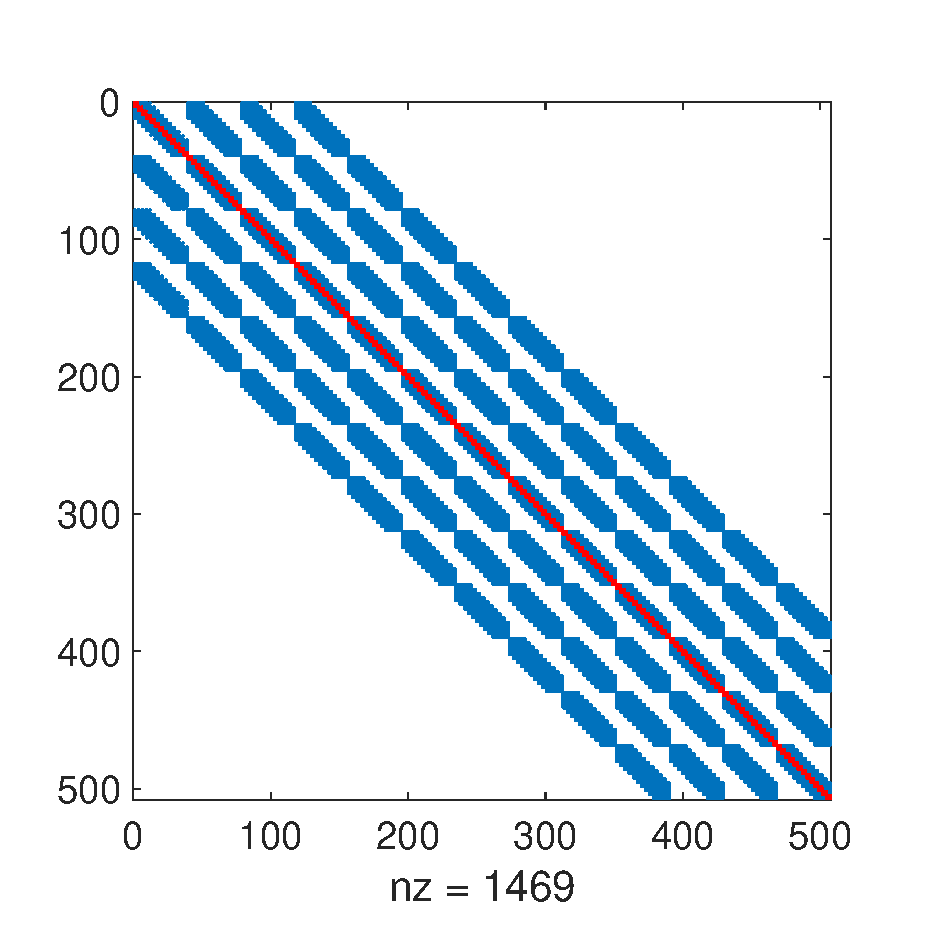
\includegraphics[width=0.45\textwidth]{Mass_matrix.eps}
	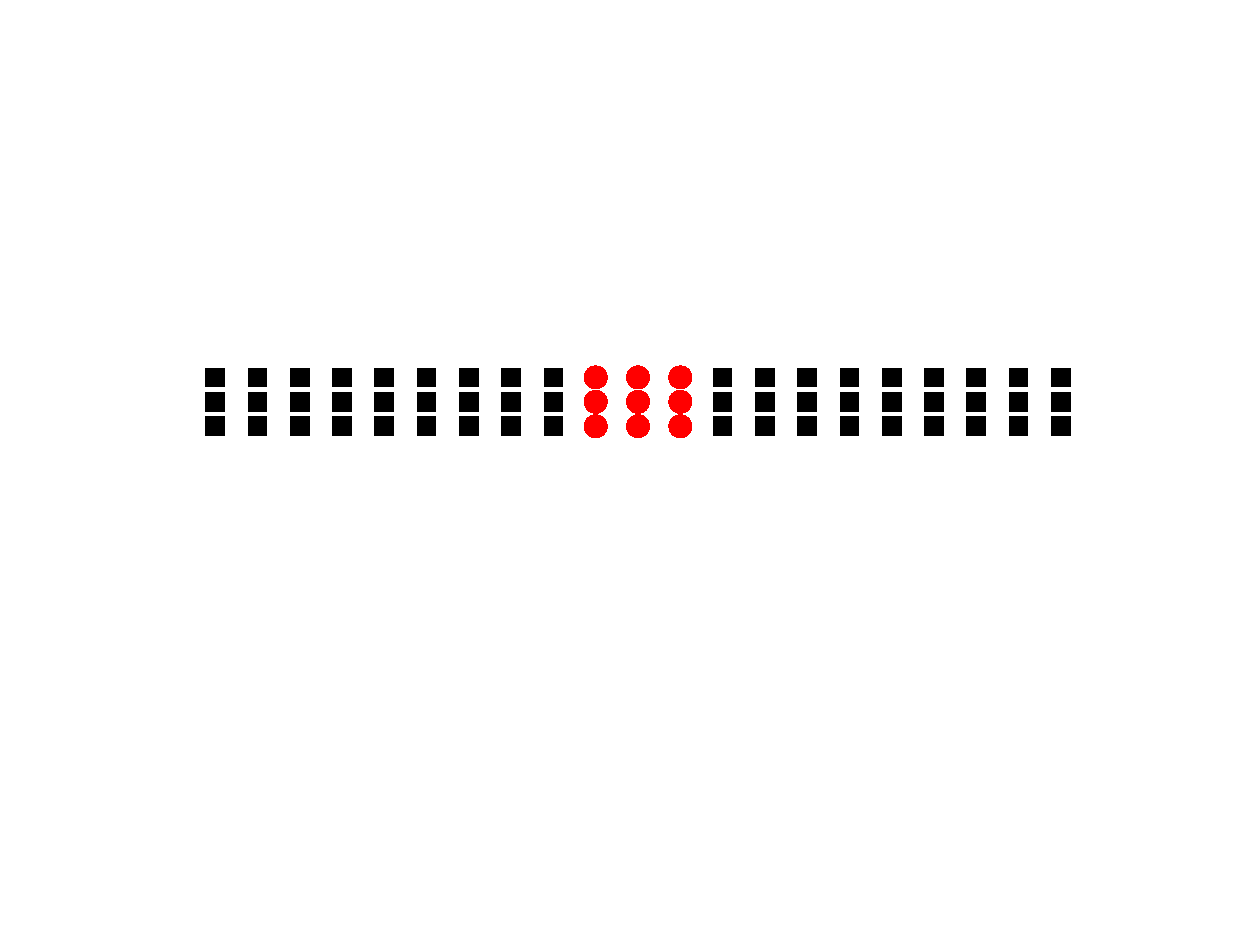
\includegraphics[width=0.45\textwidth]{Mass_block_diagonal.eps}
	\caption{The left panel is the structure of the coefficient matrix of the linear system (\ref{traction_continuous_curvi}). For each blue triangle and purple circle in the left panel, they have the structure as in the right panel which is constructed by balck squares and red circles. This wide stencile is determined by the restriction operator on interpolation operation in two dimensional.}\label{Mass_matrix}
\end{figure}


%!TEX root = SISC_elastic_3d.tex
\subsection{Gaussian source}\label{gaussian_source}
In this section, we present the numerical experiments to illustrate that there is no obvious artifacts are generated by the curvilinear interface. For coarse domain, it is set to be
\[ {\bf x} = {\bf X}^c({\bf r}) = \left(\begin{array}{c}
2000 r^{(1)}\\
2000 r^{(2)}\\
r^{(3)} \theta_i\big(r^{(1)}, r^{(2)}\big) + (1-r^{(3)}) \theta_b\big(r^{(1)},r^{(2)}\big) \end{array}\right). \]
Here, $0\leq r^{(1)}, r^{(2)}, r^{(3)}\leq 1$, $\theta_i$ is the interface surface geometry,
\begin{equation}\label{interface_gausian}
\theta_i\big(r^{(1)},r^{(2)}\big) = 800+20\sin(4\pi r^{(1)})+20\cos(4\pi r^{(2)}),
\end{equation}
and 
$\theta_b$ is the bottom surface geometry,
\begin{equation*}
\theta_b\big(r^{(1)},r^{(2)}\big) = 0.
\end{equation*}
As for the fine domain $\Omega^f$, we choose it to be
\[ {\bf x} = {\bf X}^f({\bf r}) = \left(\begin{array}{c}
2000 r^{(1)}\\
2000 r^{(2)}\\
r^{(3)}\theta_t\big(r^{(1)},r^{(2)}\big) + (1-r^{(3)})\theta_i\big(r^{(1)},r^{(2)}\big)\end{array}\right). \]
Here, $0\leq r^{(1)}, r^{(2)}, r^{(3)}\leq 1$, $\theta_t$ is the top surface geometry,
\begin{equation*}
\theta_t\big(r^{(1)},r^{(2)}\big) = 1000,
\end{equation*}
and $\theta_i$ is the interface geometry which is given in (\ref{interface_gausian}). For both fine and coarse domains, let the density vary according to
\begin{equation*}
\rho(x^{(1)},x^{(2)},x^{(3)}) = 1.5\times 10^3,
\end{equation*}
and material parameters $\mu, \lambda$ satisfy
\begin{equation*}
\mu(x^{(1)},x^{(2)},x^{(3)}) = 1.5\times 10^9,\ \ 
\lambda(x^{(1)},x^{(2)},x^{(3)})  = 3\times 10^9,
\end{equation*}
respectively. In addition, we impose a Gaussian source on the top surface
\[{\bf g} = (g_1,g_2,g_3)^T ,\]
where, $g_1 = g_2 = 0$, and 
\[g_3 = 10^9 \text{exp}\left(-\left(\frac{t-4/44.2}{1/44.2}\right)^2\right)\text{exp}\left(-\left(\frac{x^{(1)}-1000}{12.5}\right)^2-\left(\frac{x^{(2)}-1000}{12.5}\right)^2\right).\]

Homogeneous Dirichlet boundary conditions are imposed on other boundaries. The external forcing is chosen to be zero everywhere and the initial conditions are also set to be zero everywhere, ${\bf u} = {\bf 0}$ at $t = 0$.

In the simulation of the reference solution, we choose $n_1 = n_2 = 201, n_3 = 101$. In the experiments for the curvilinear interface with mesh refinement, we have $n_1^{2h} = n_2^{2h} = 101, n_3^{2h} = 41$ and $n_1^h = n_2^h = 201, n_3^h = 21$. The final simulation time is $T = 0.4$.

\begin{figure}[htbp]
	\centering
	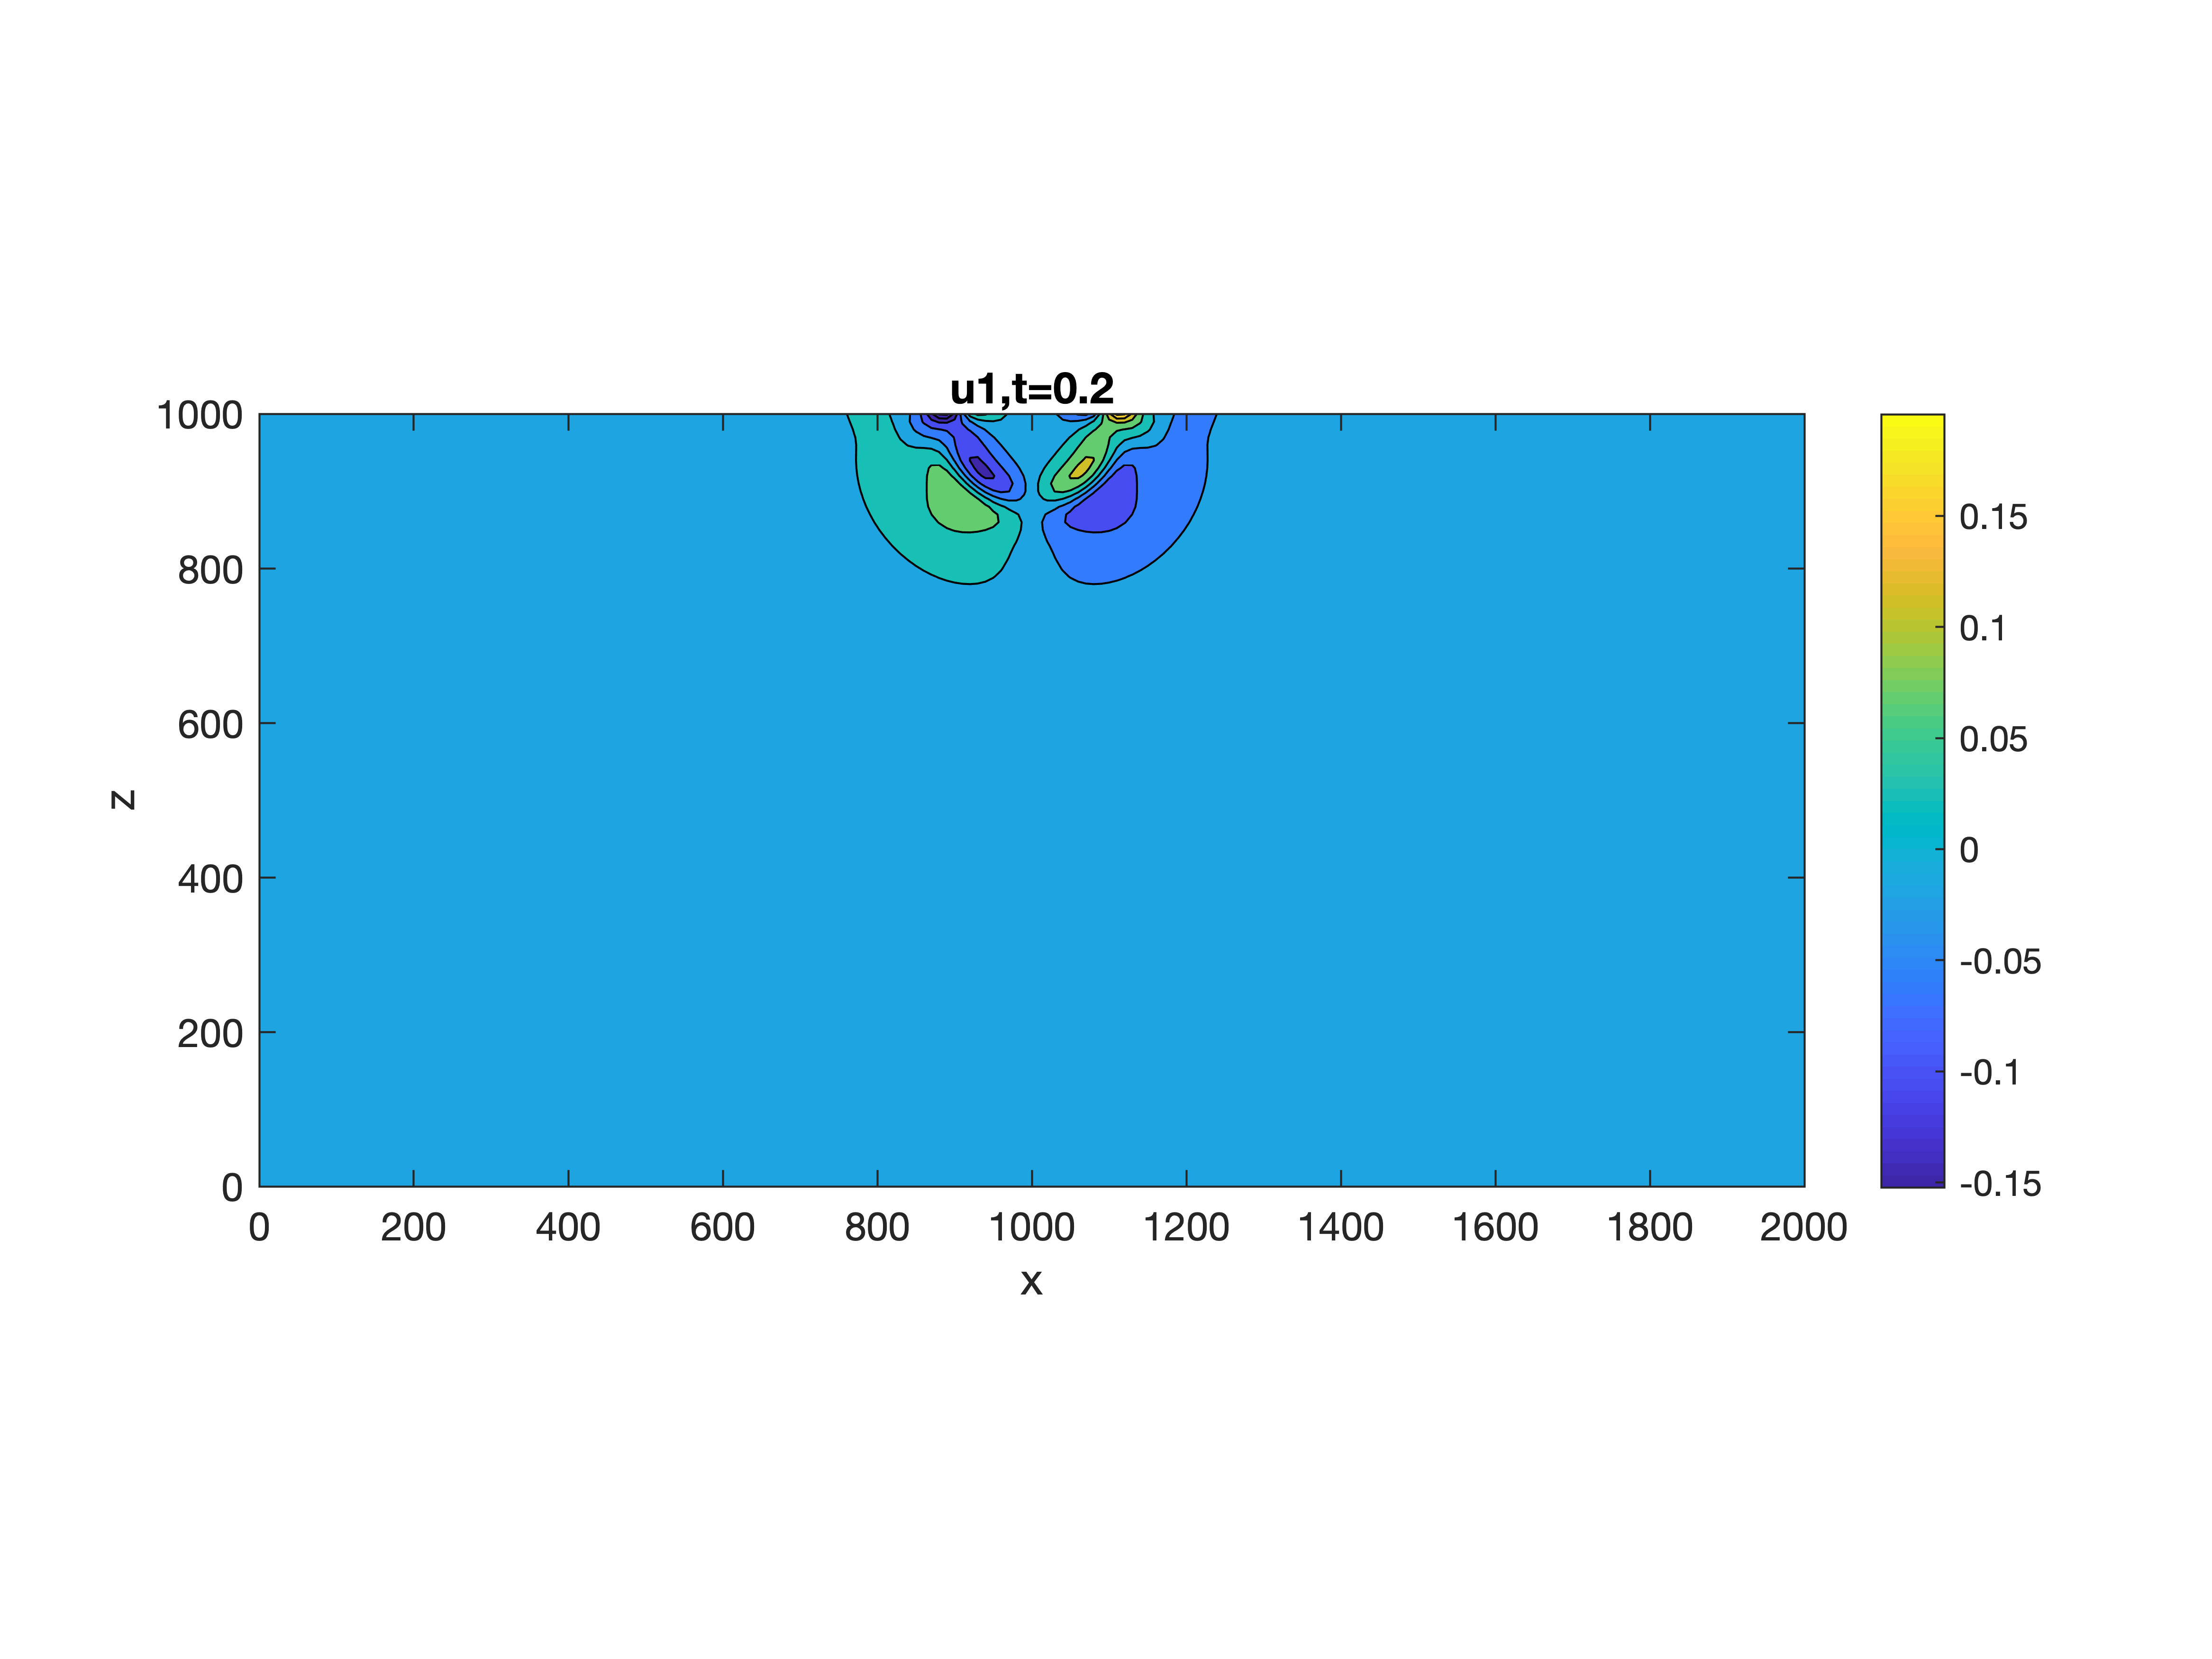
\includegraphics[width=0.4\textwidth,trim={0 2.8cm 0 2.8cm}, clip]{u1_t02_cartesian.png}
	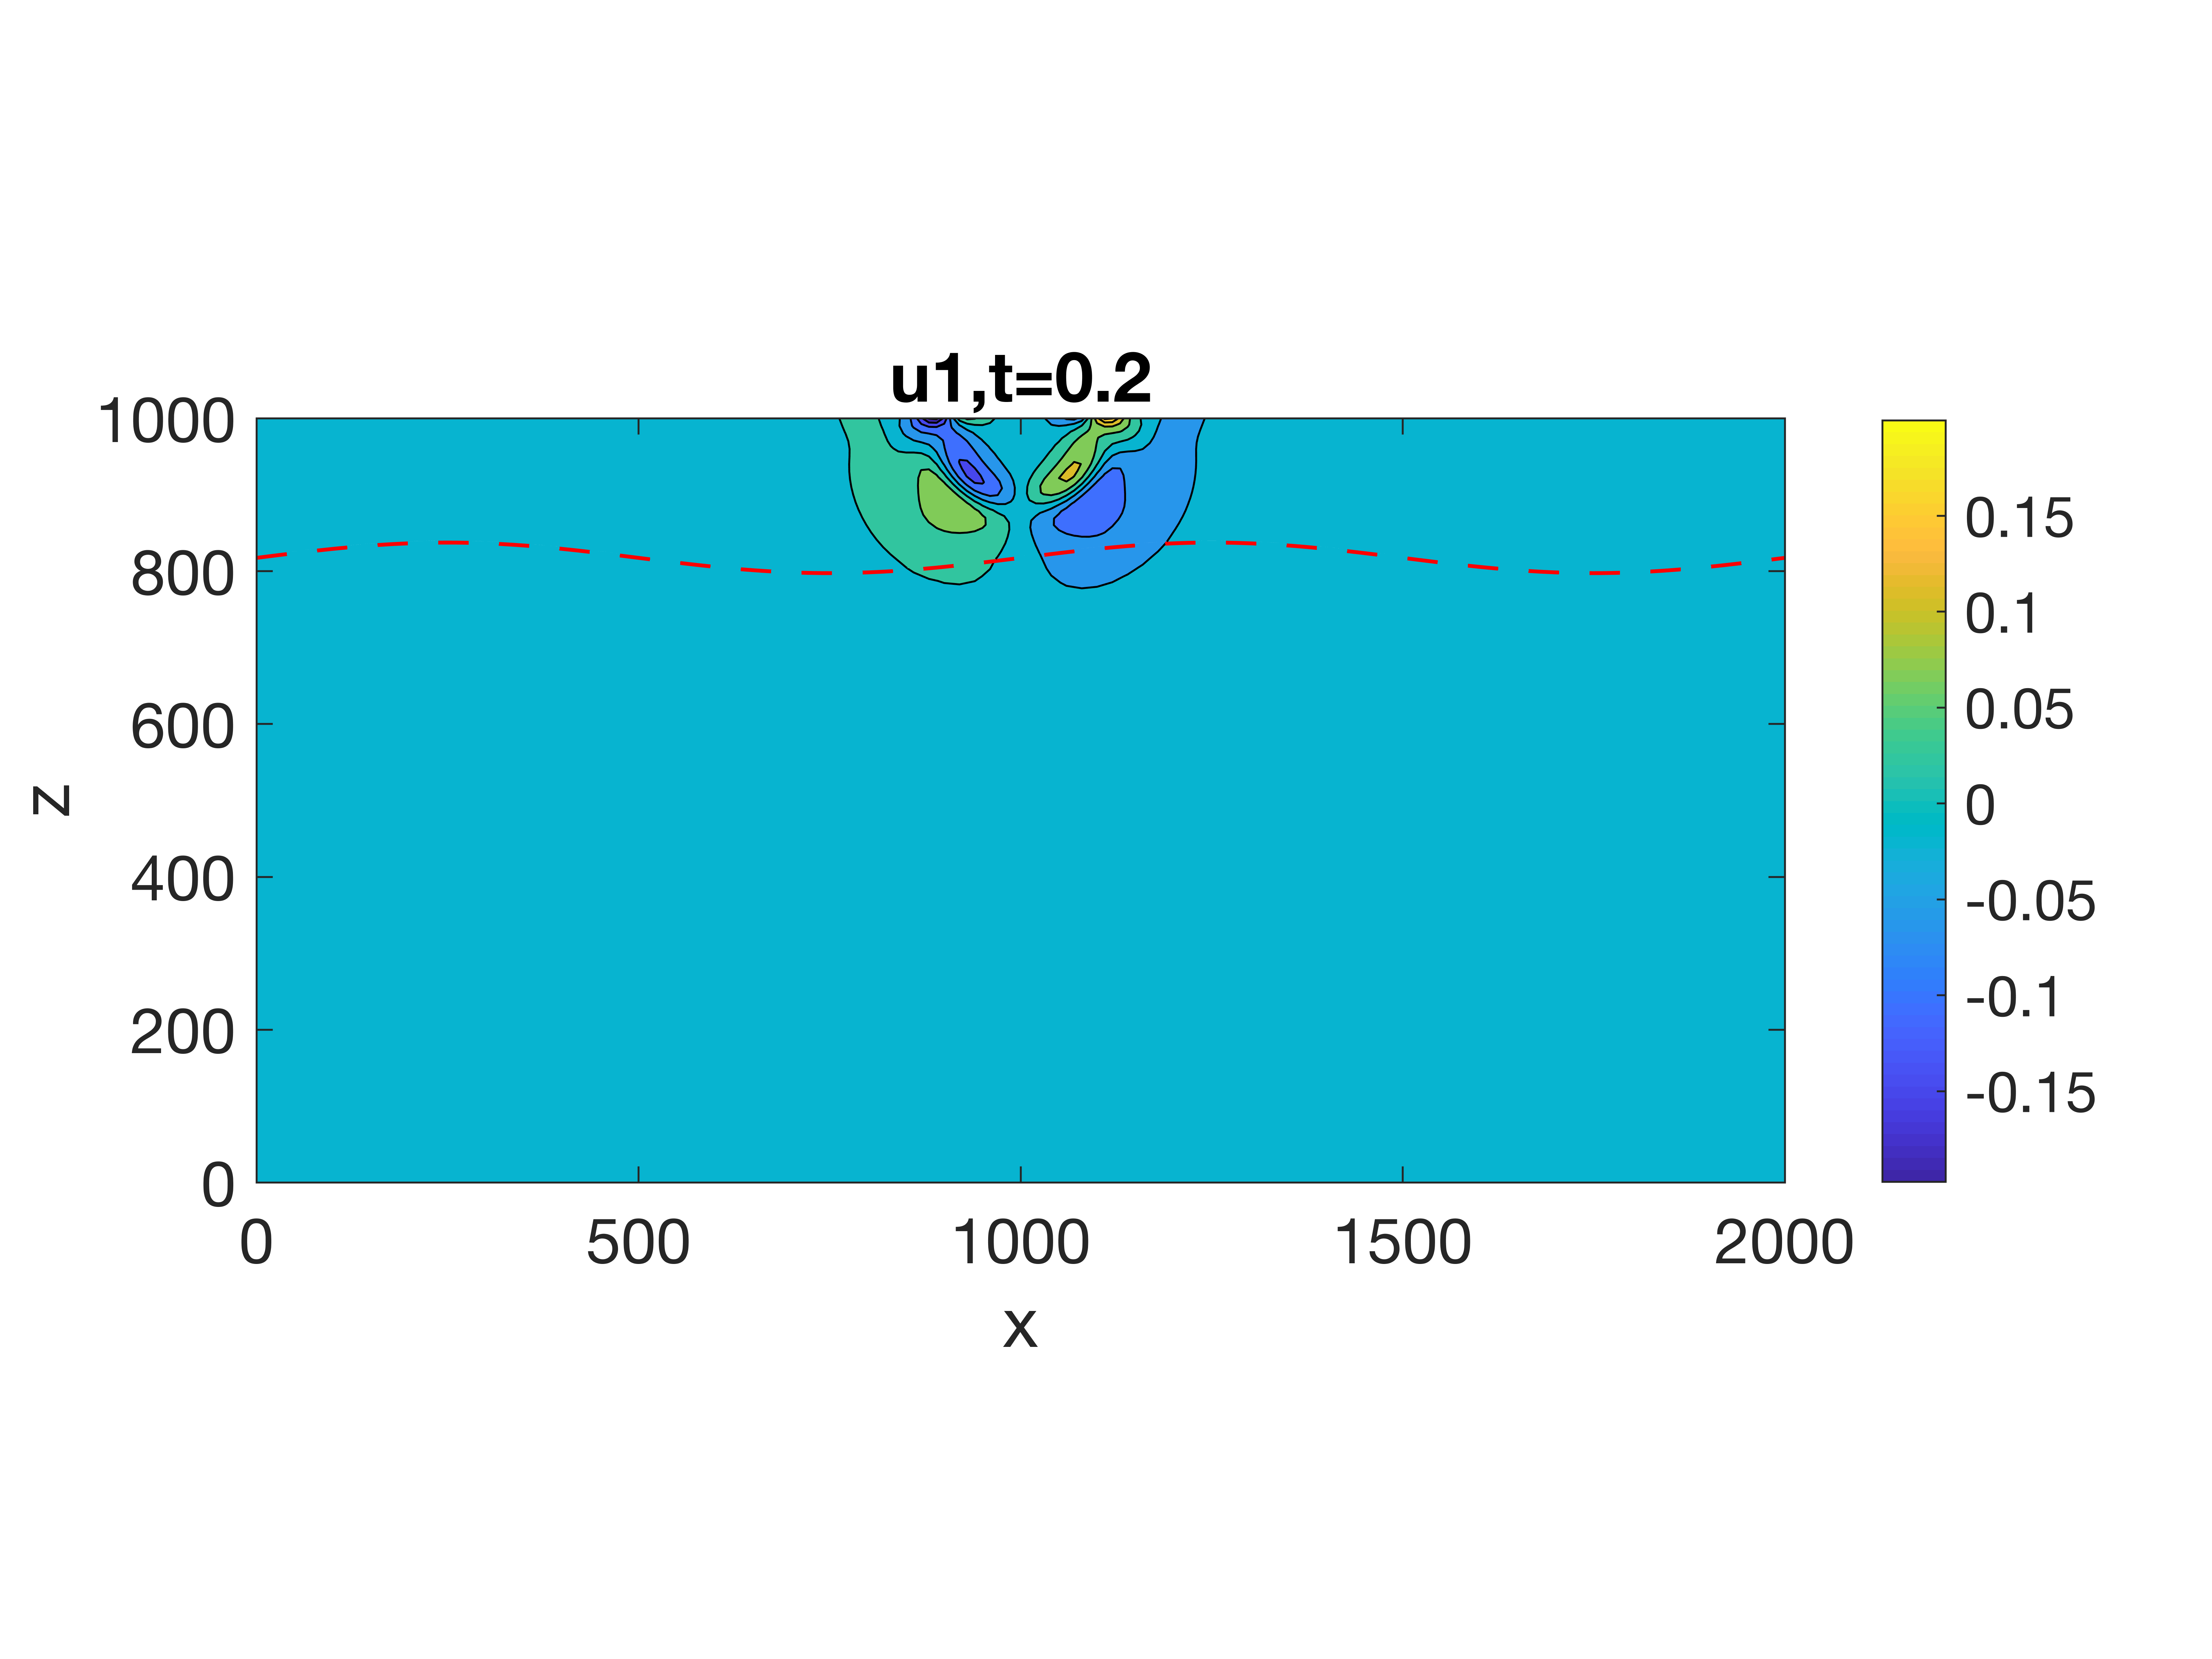
\includegraphics[width=0.4\textwidth,trim={0 2.8cm 0 2.8cm}, clip]{u1_t02_curvi_mr.png}\\
	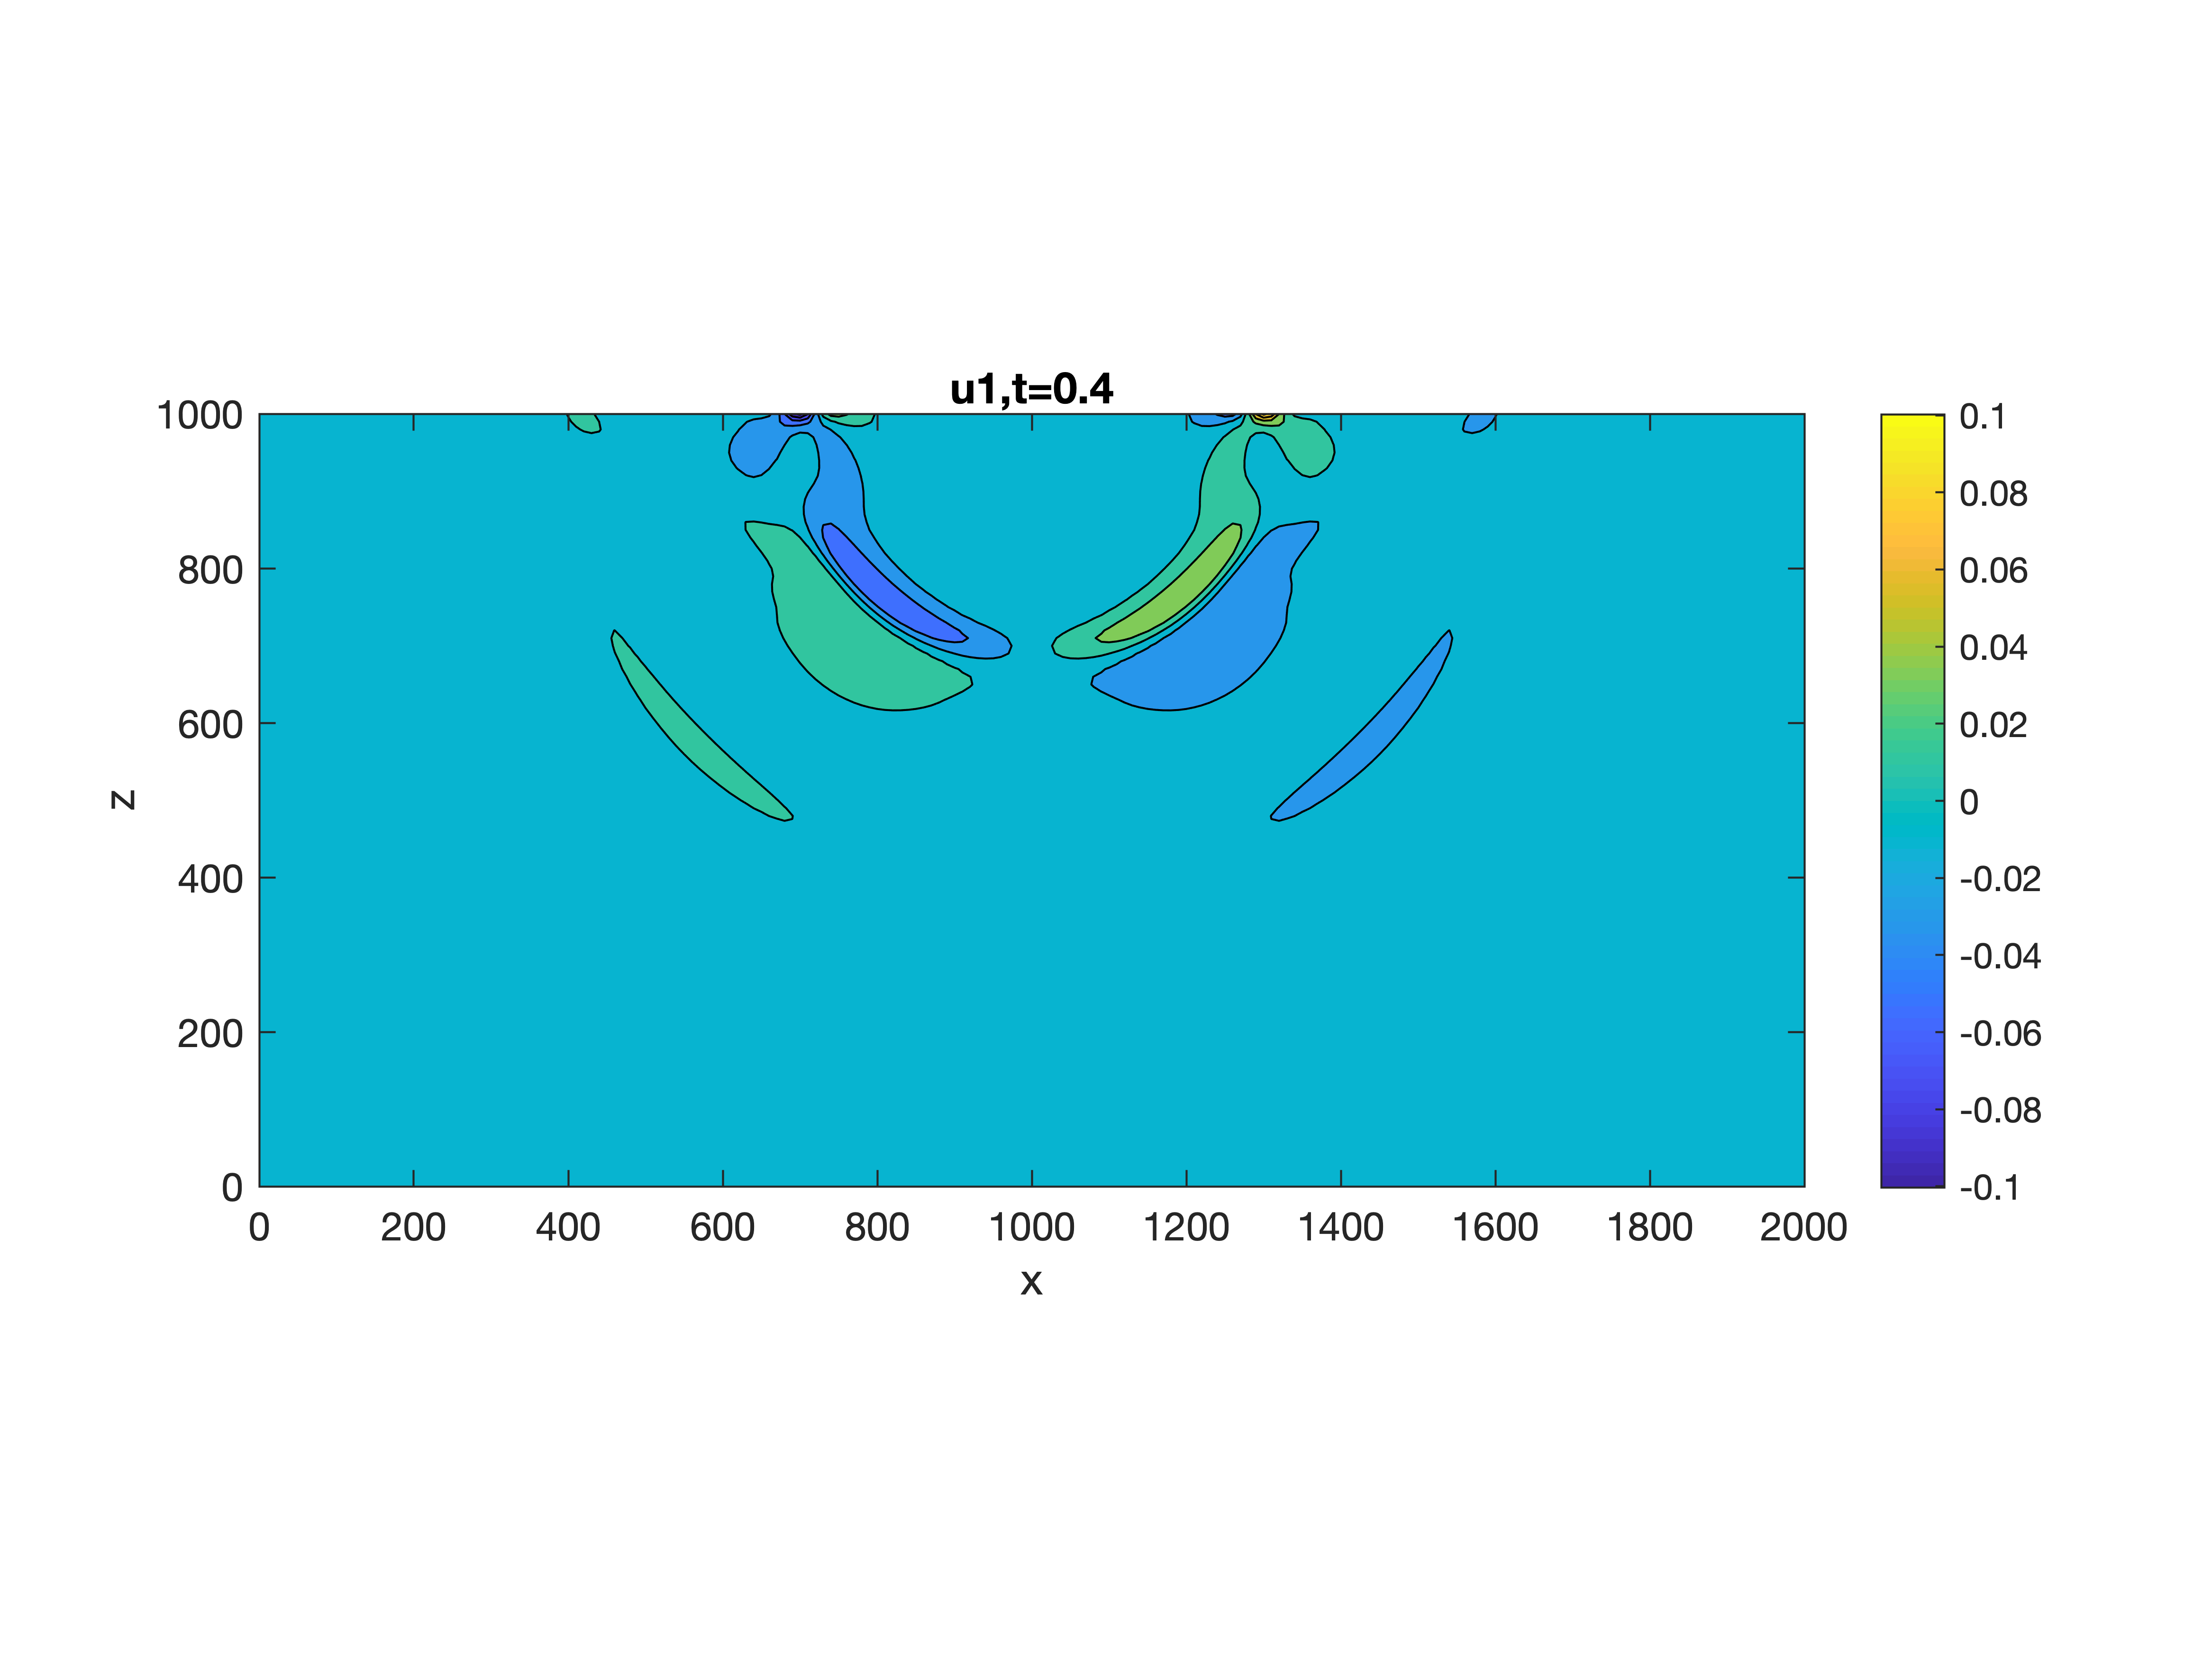
\includegraphics[width=0.4\textwidth,trim={0 2.8cm 0 2.8cm}, clip]{u1_t04_cartesian.png}
	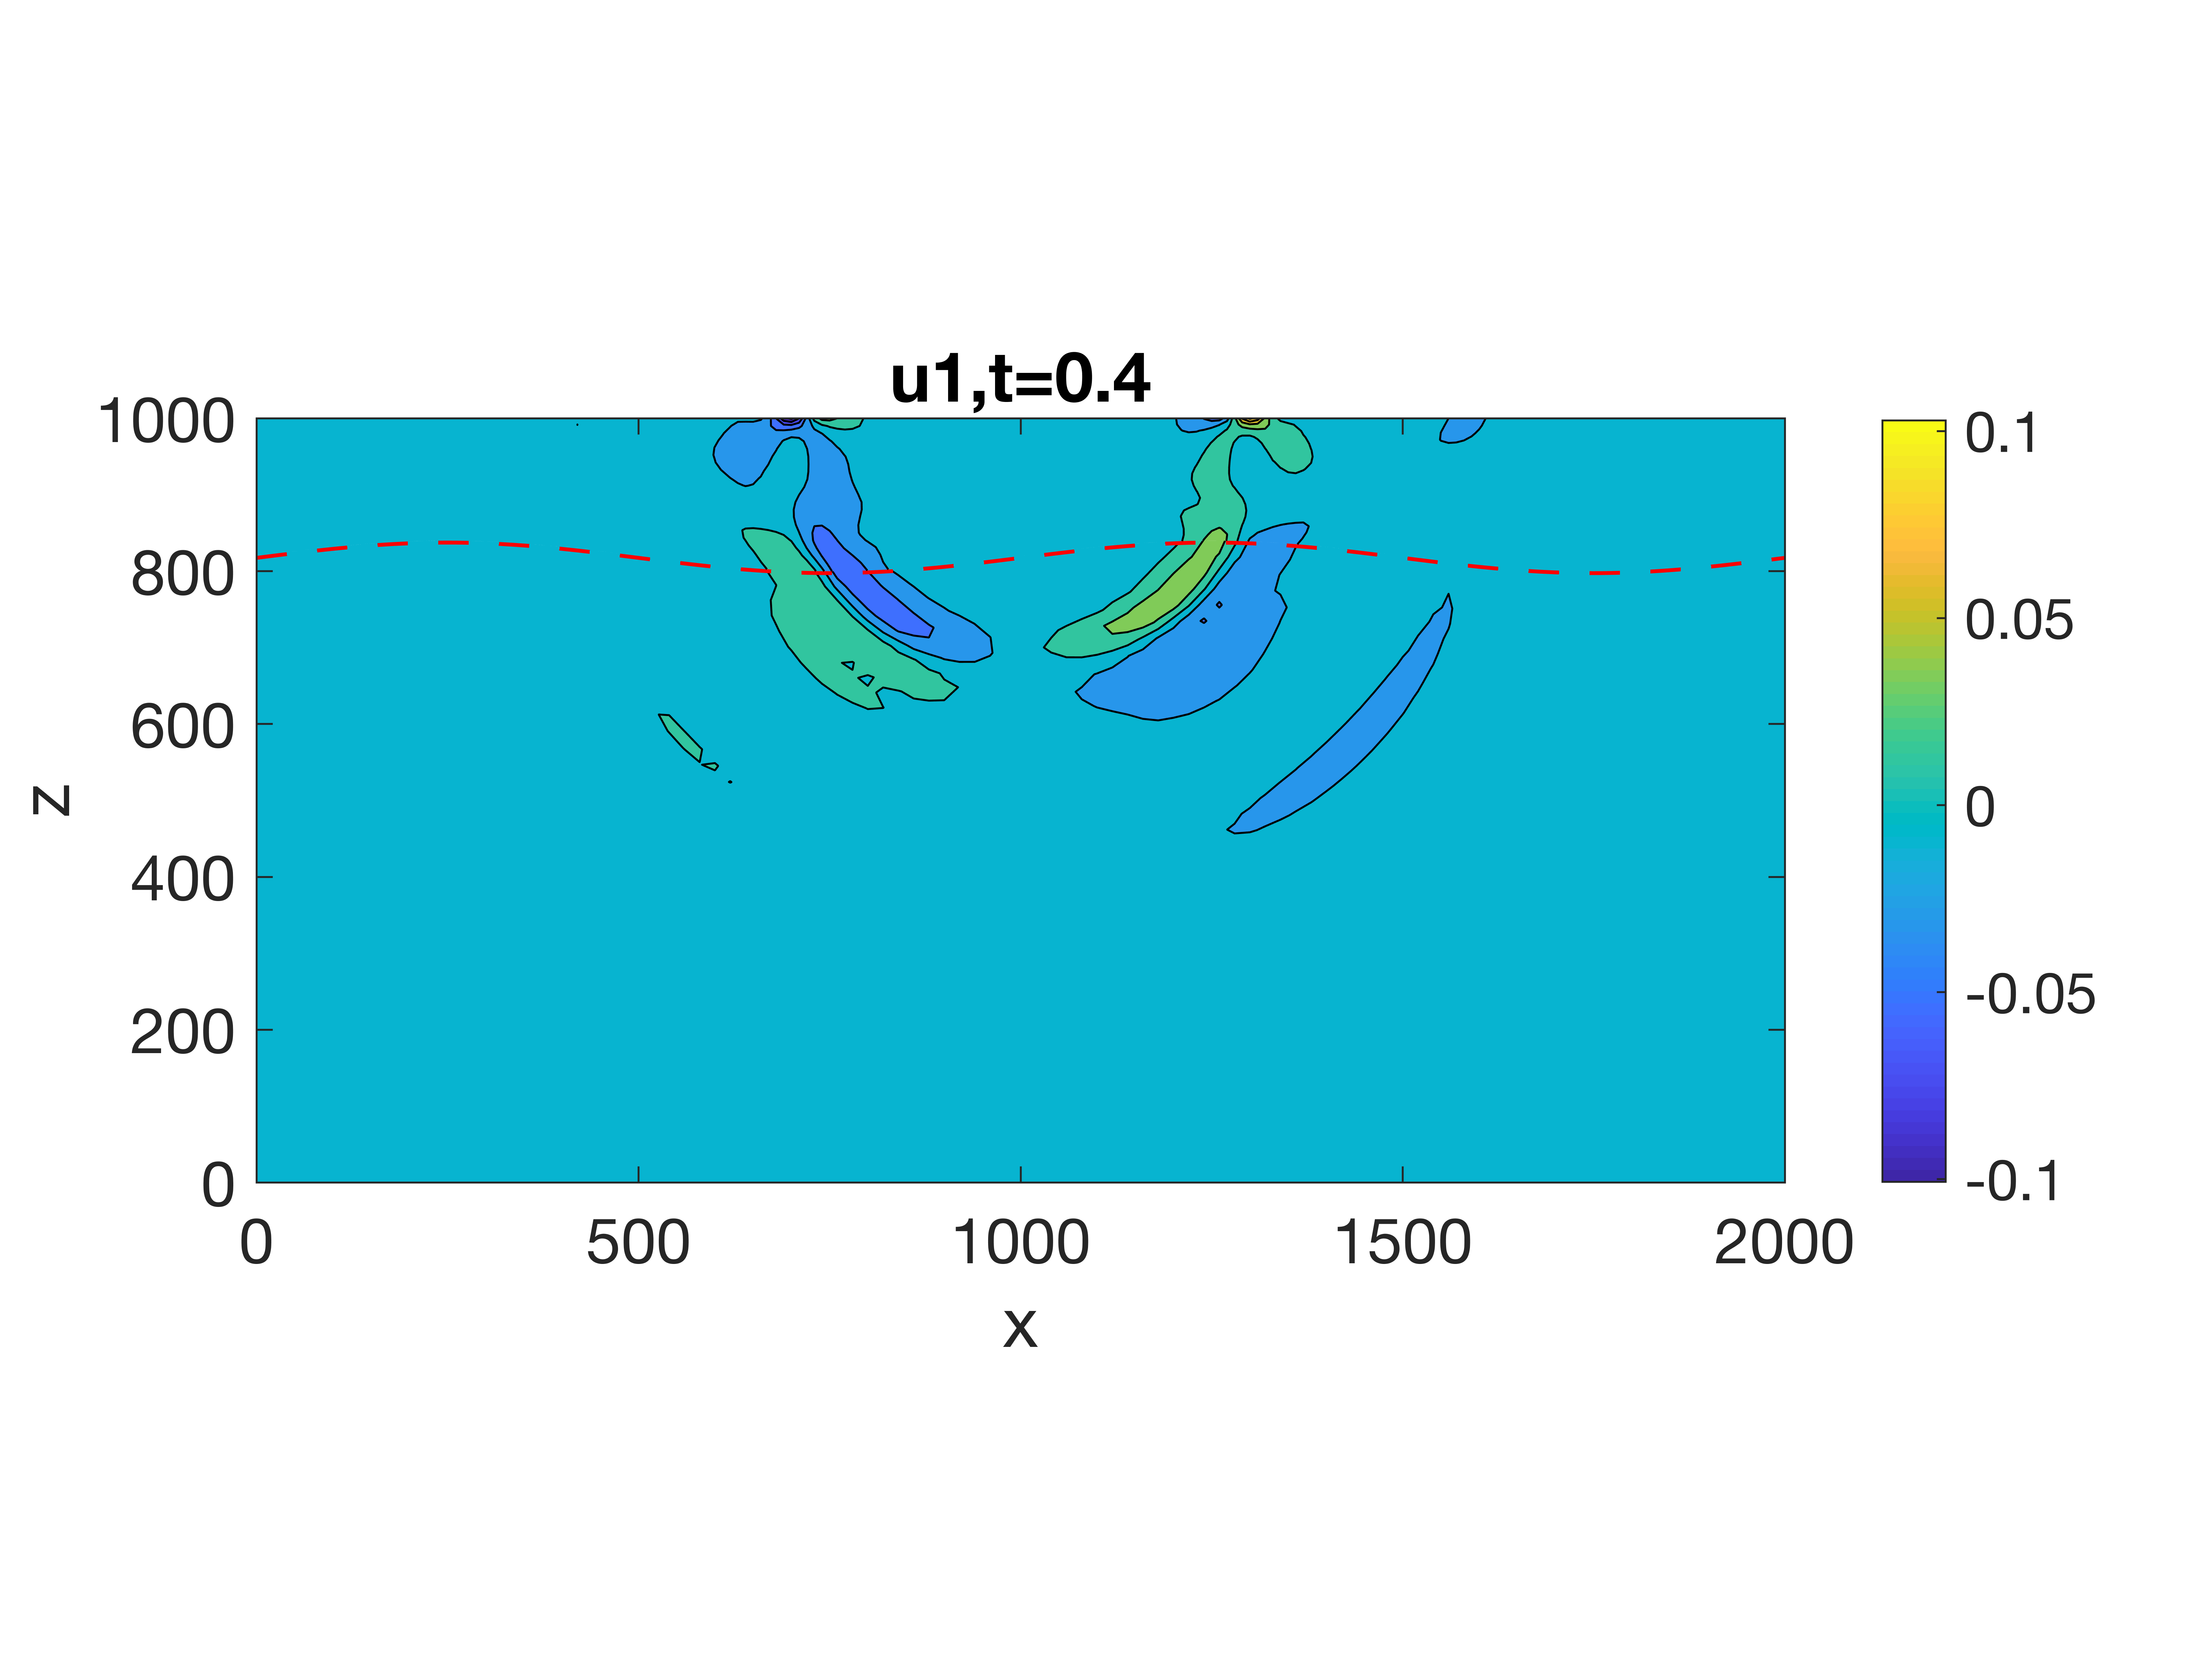
\includegraphics[width=0.4\textwidth,trim={0 2.8cm 0 2.8cm}, clip]{u1_t04_curvi_mr.png}
\caption{The graphs for $u_1$. In the two figures on the left, we show reference solutions at $t=0.2$ and $t=0.4$, computed on a Cartesian mesh without mesh refinement interface. On the right, the two figures show the solutions computed on a curvilinear mesh with a curved mesh refinement interface at $t=0.2$ and $t=0.4$. The curved interfaces are marked with the red dash lines. Note that $x,z$ in the graph correspond to $x^{(1)}, x^{(3)}$ respectively.}
\label{u1}
\end{figure}

%\begin{figure}[htbp]
%	\centering
%	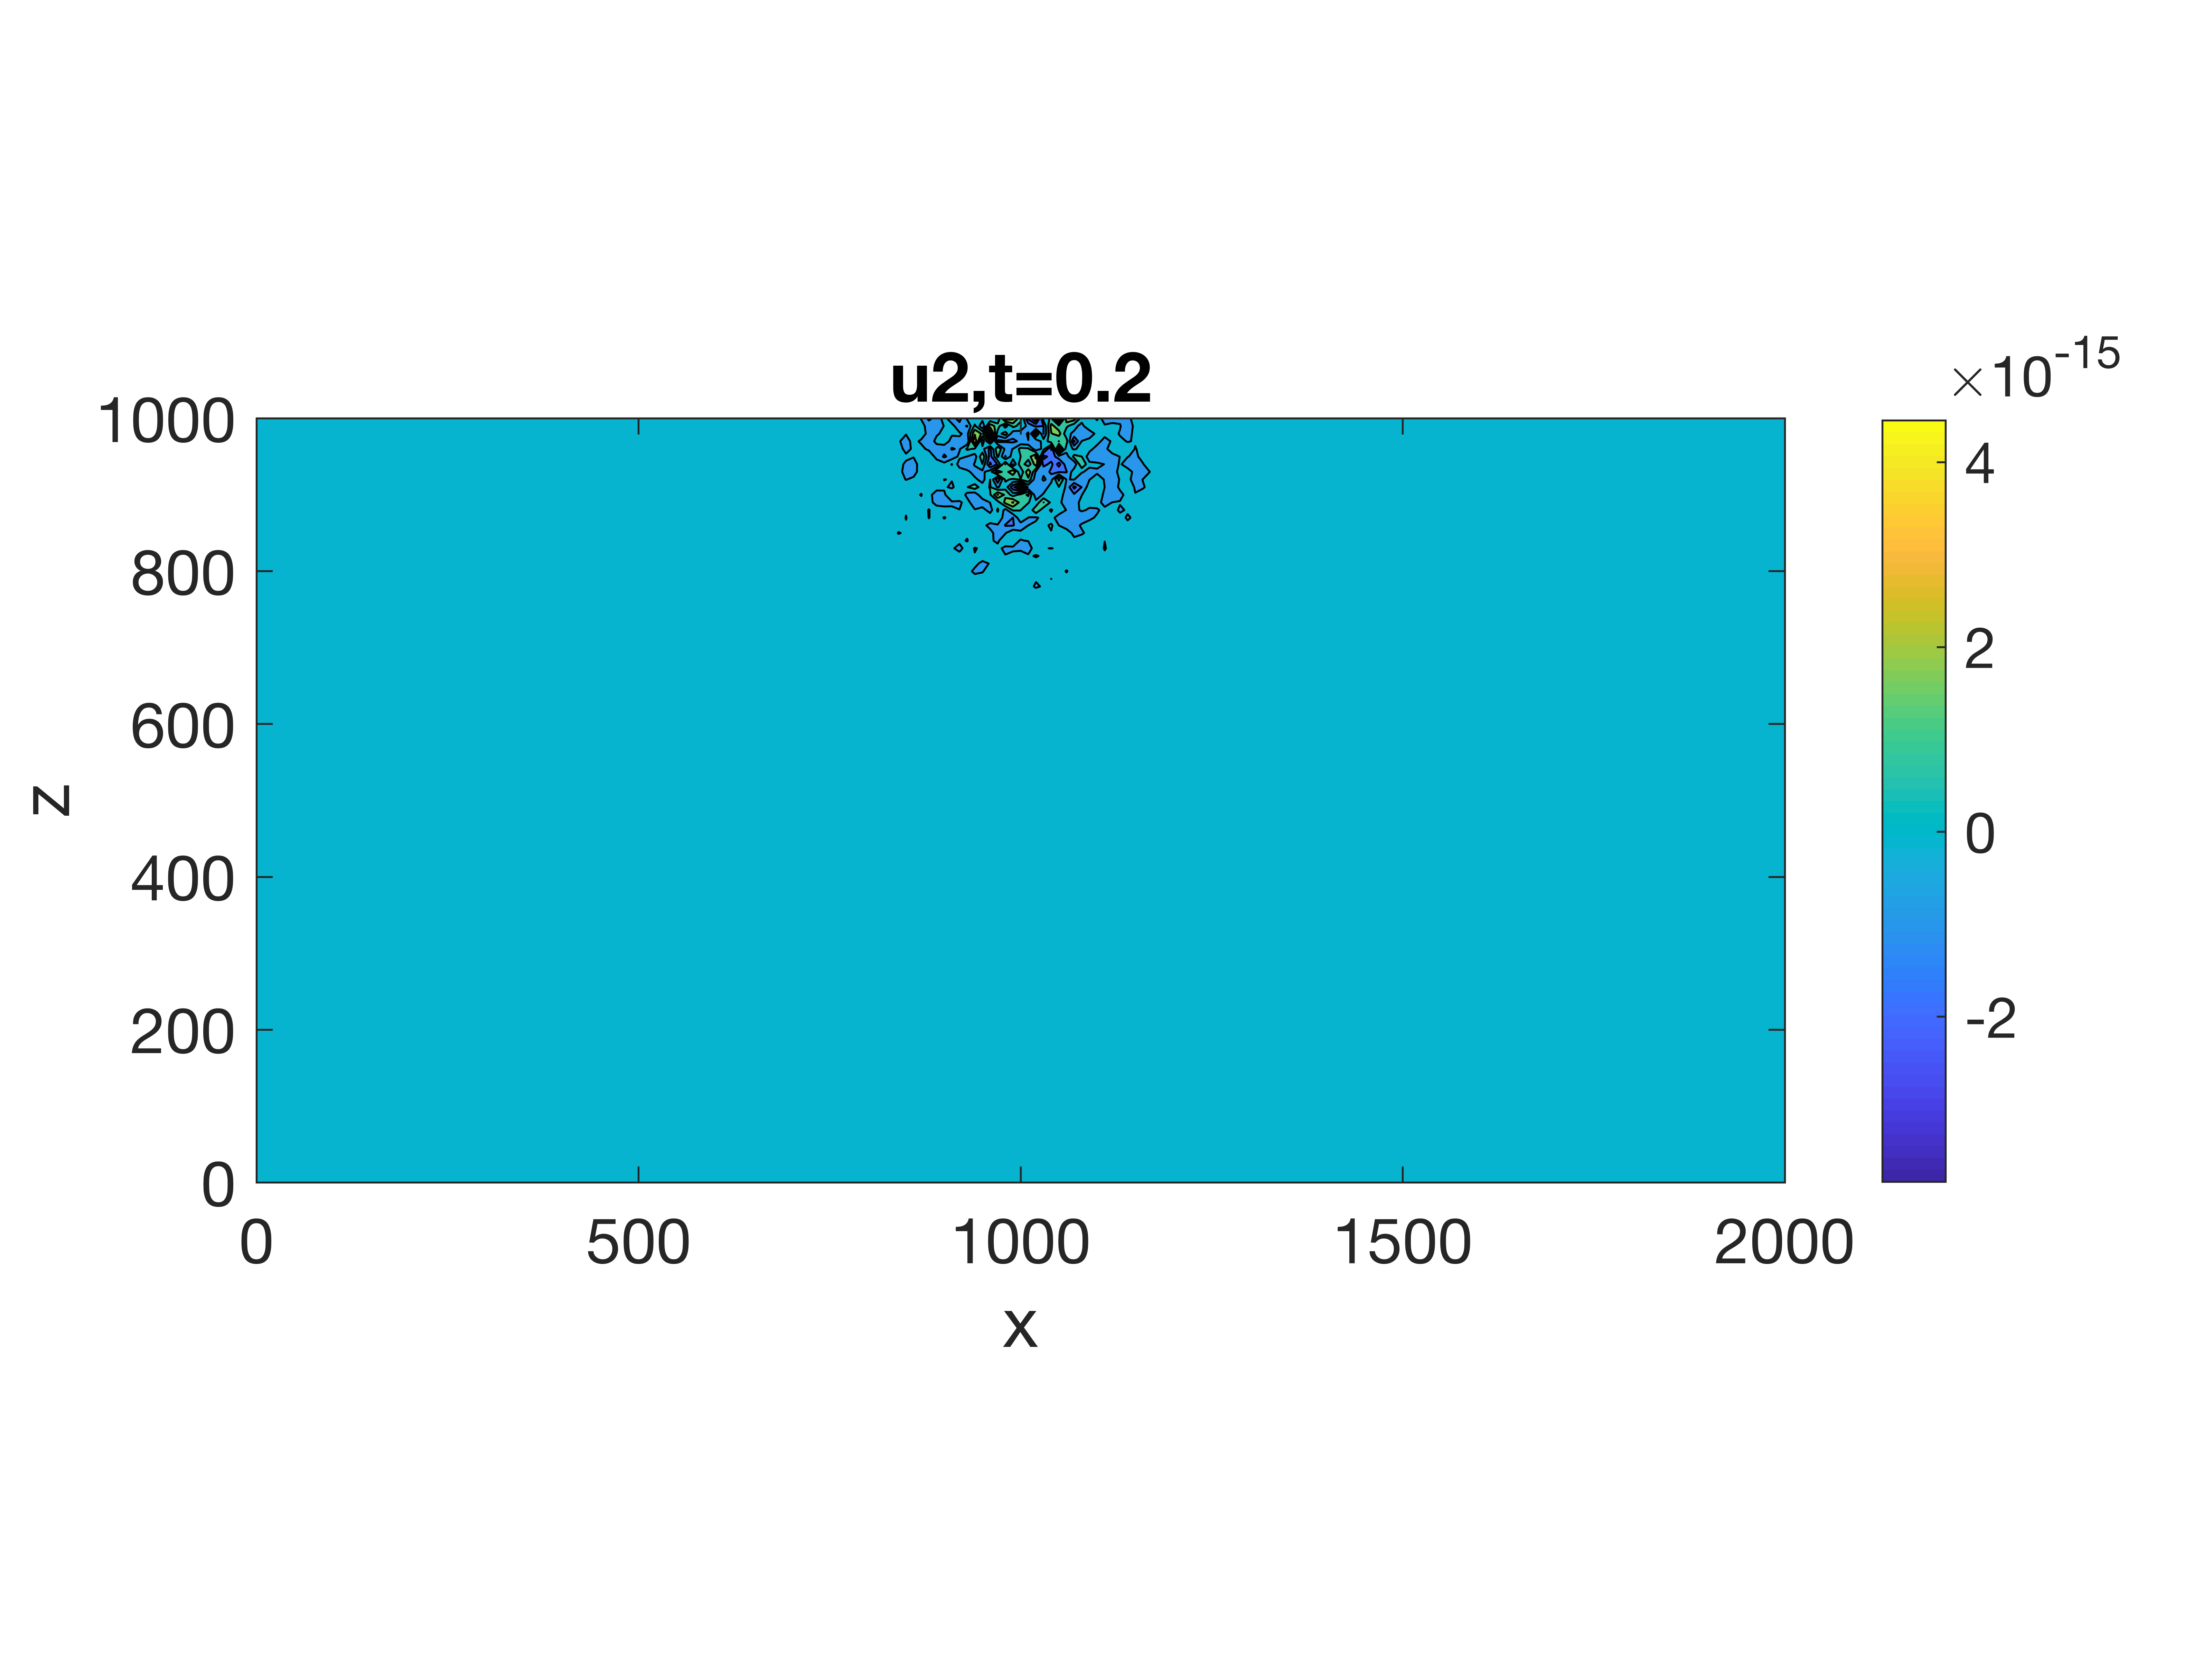
\includegraphics[width=0.4\textwidth,trim={0 2.8cm 0 2.8cm}, clip]{u2_t02_cartesian.png}
%	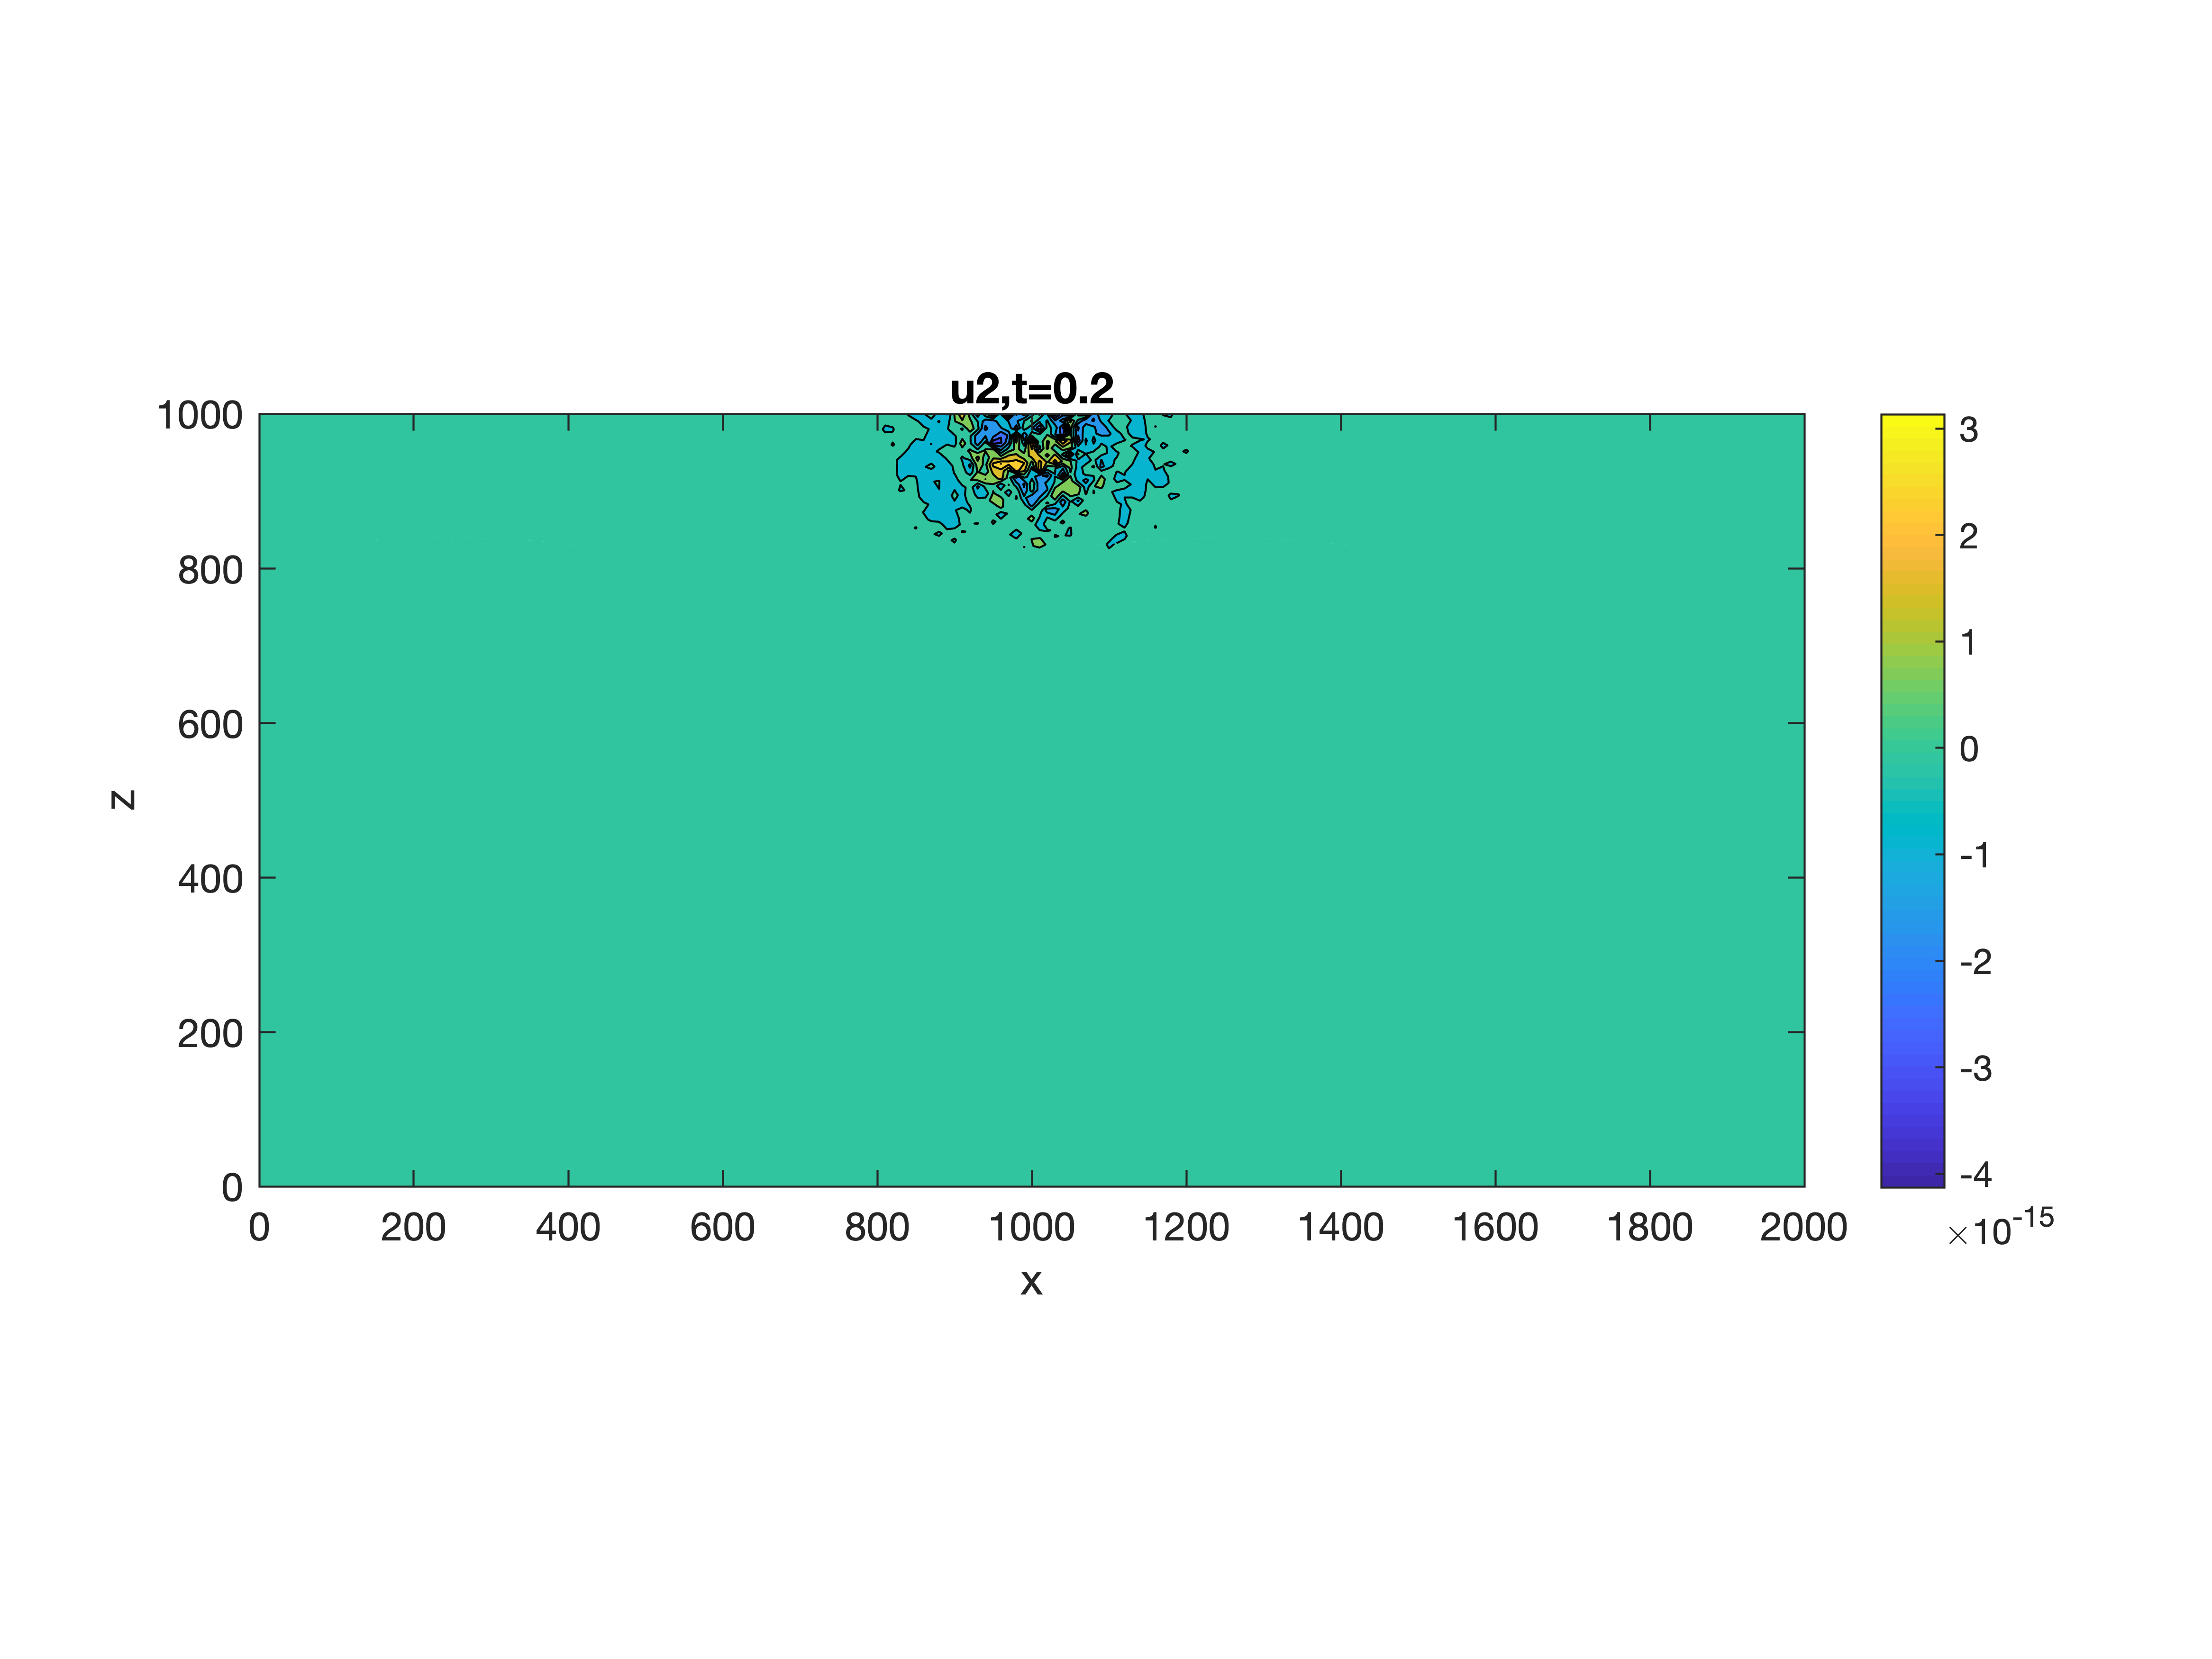
\includegraphics[width=0.4\textwidth,trim={0 2.8cm 0 2.8cm}, clip]{u2_t02_curvi_mr.png}\\
%	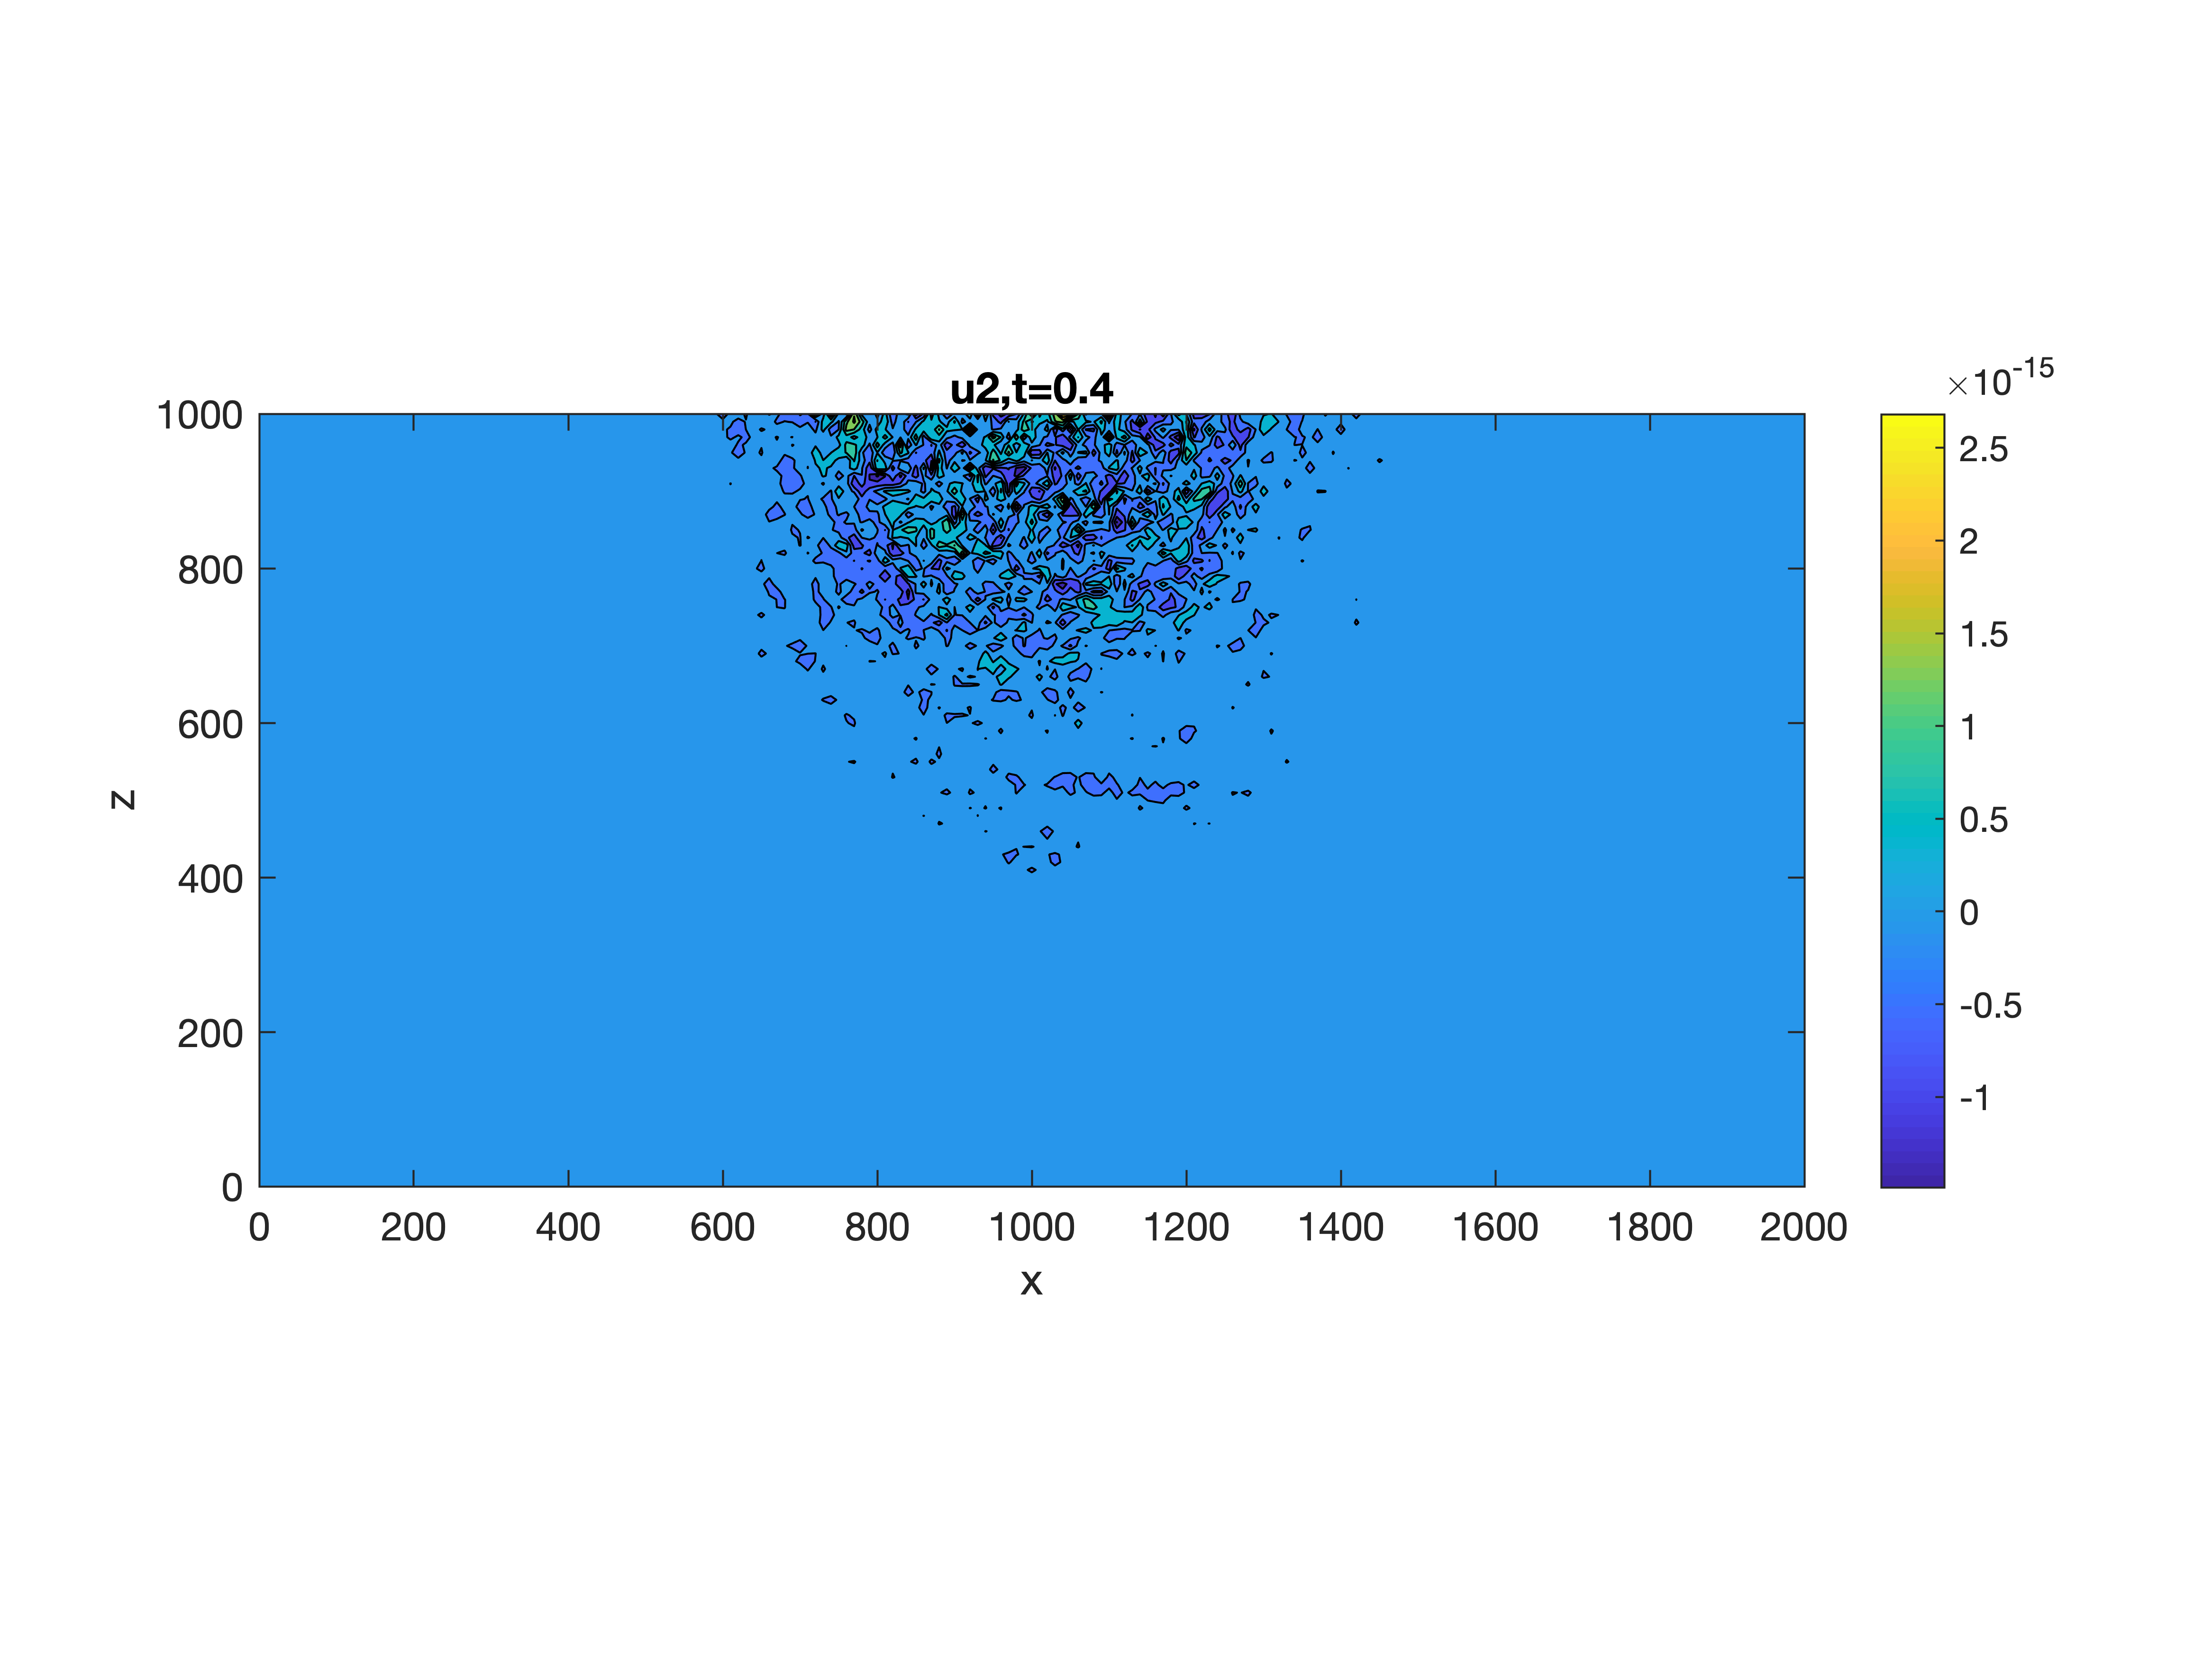
\includegraphics[width=0.4\textwidth,trim={0 2.8cm 0 2.8cm}, clip]{u2_t04_cartesian.png}
%	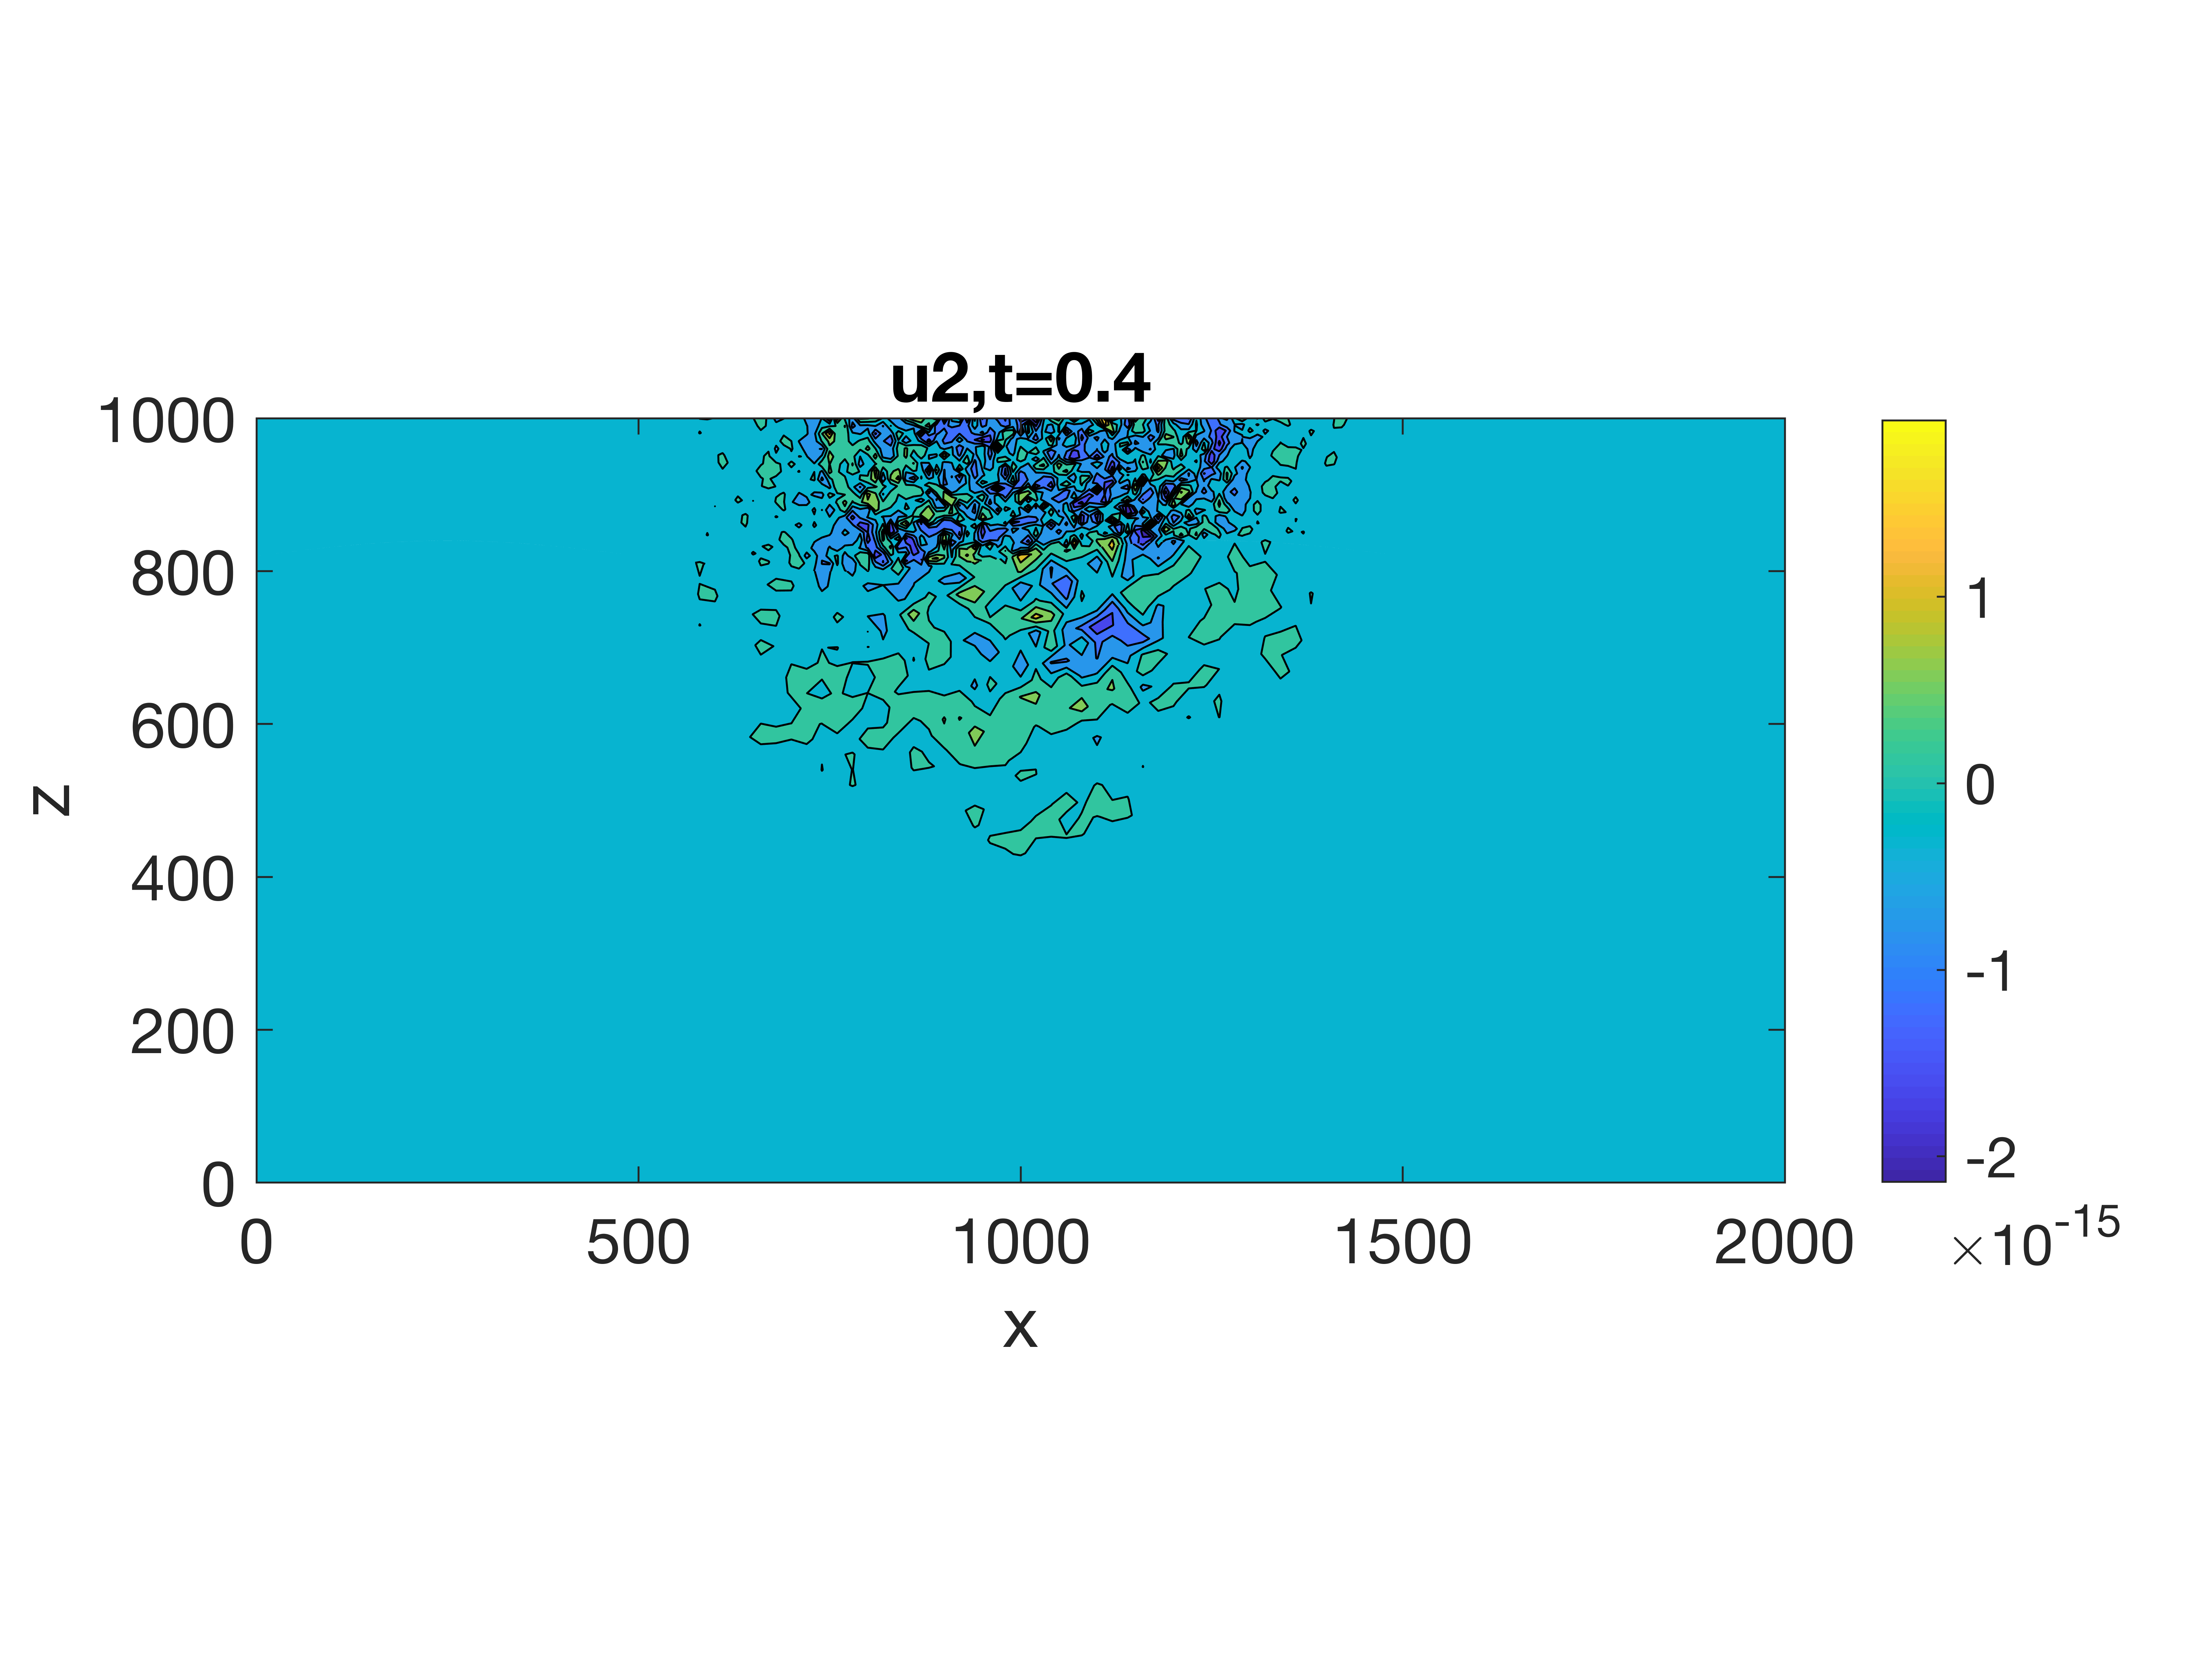
\includegraphics[width=0.4\textwidth,trim={0 2.8cm 0 2.8cm}, clip]{u2_t04_curvi_mr.png}
%	\caption{The graph for $u_2$. From left to right are for Cartesian mesh without mesh refinement interface and curvilinear mesh with mesh refinement interface respectively. From top to bottom are for $t = 0.2$ and $t = 0.4$ respectively. Note that $x,z$ in the graph correspond to $x^{(1)}, x^{(3)}$ respectively.}\label{u2}
%\end{figure}

\begin{figure}[htbp]
	\centering
	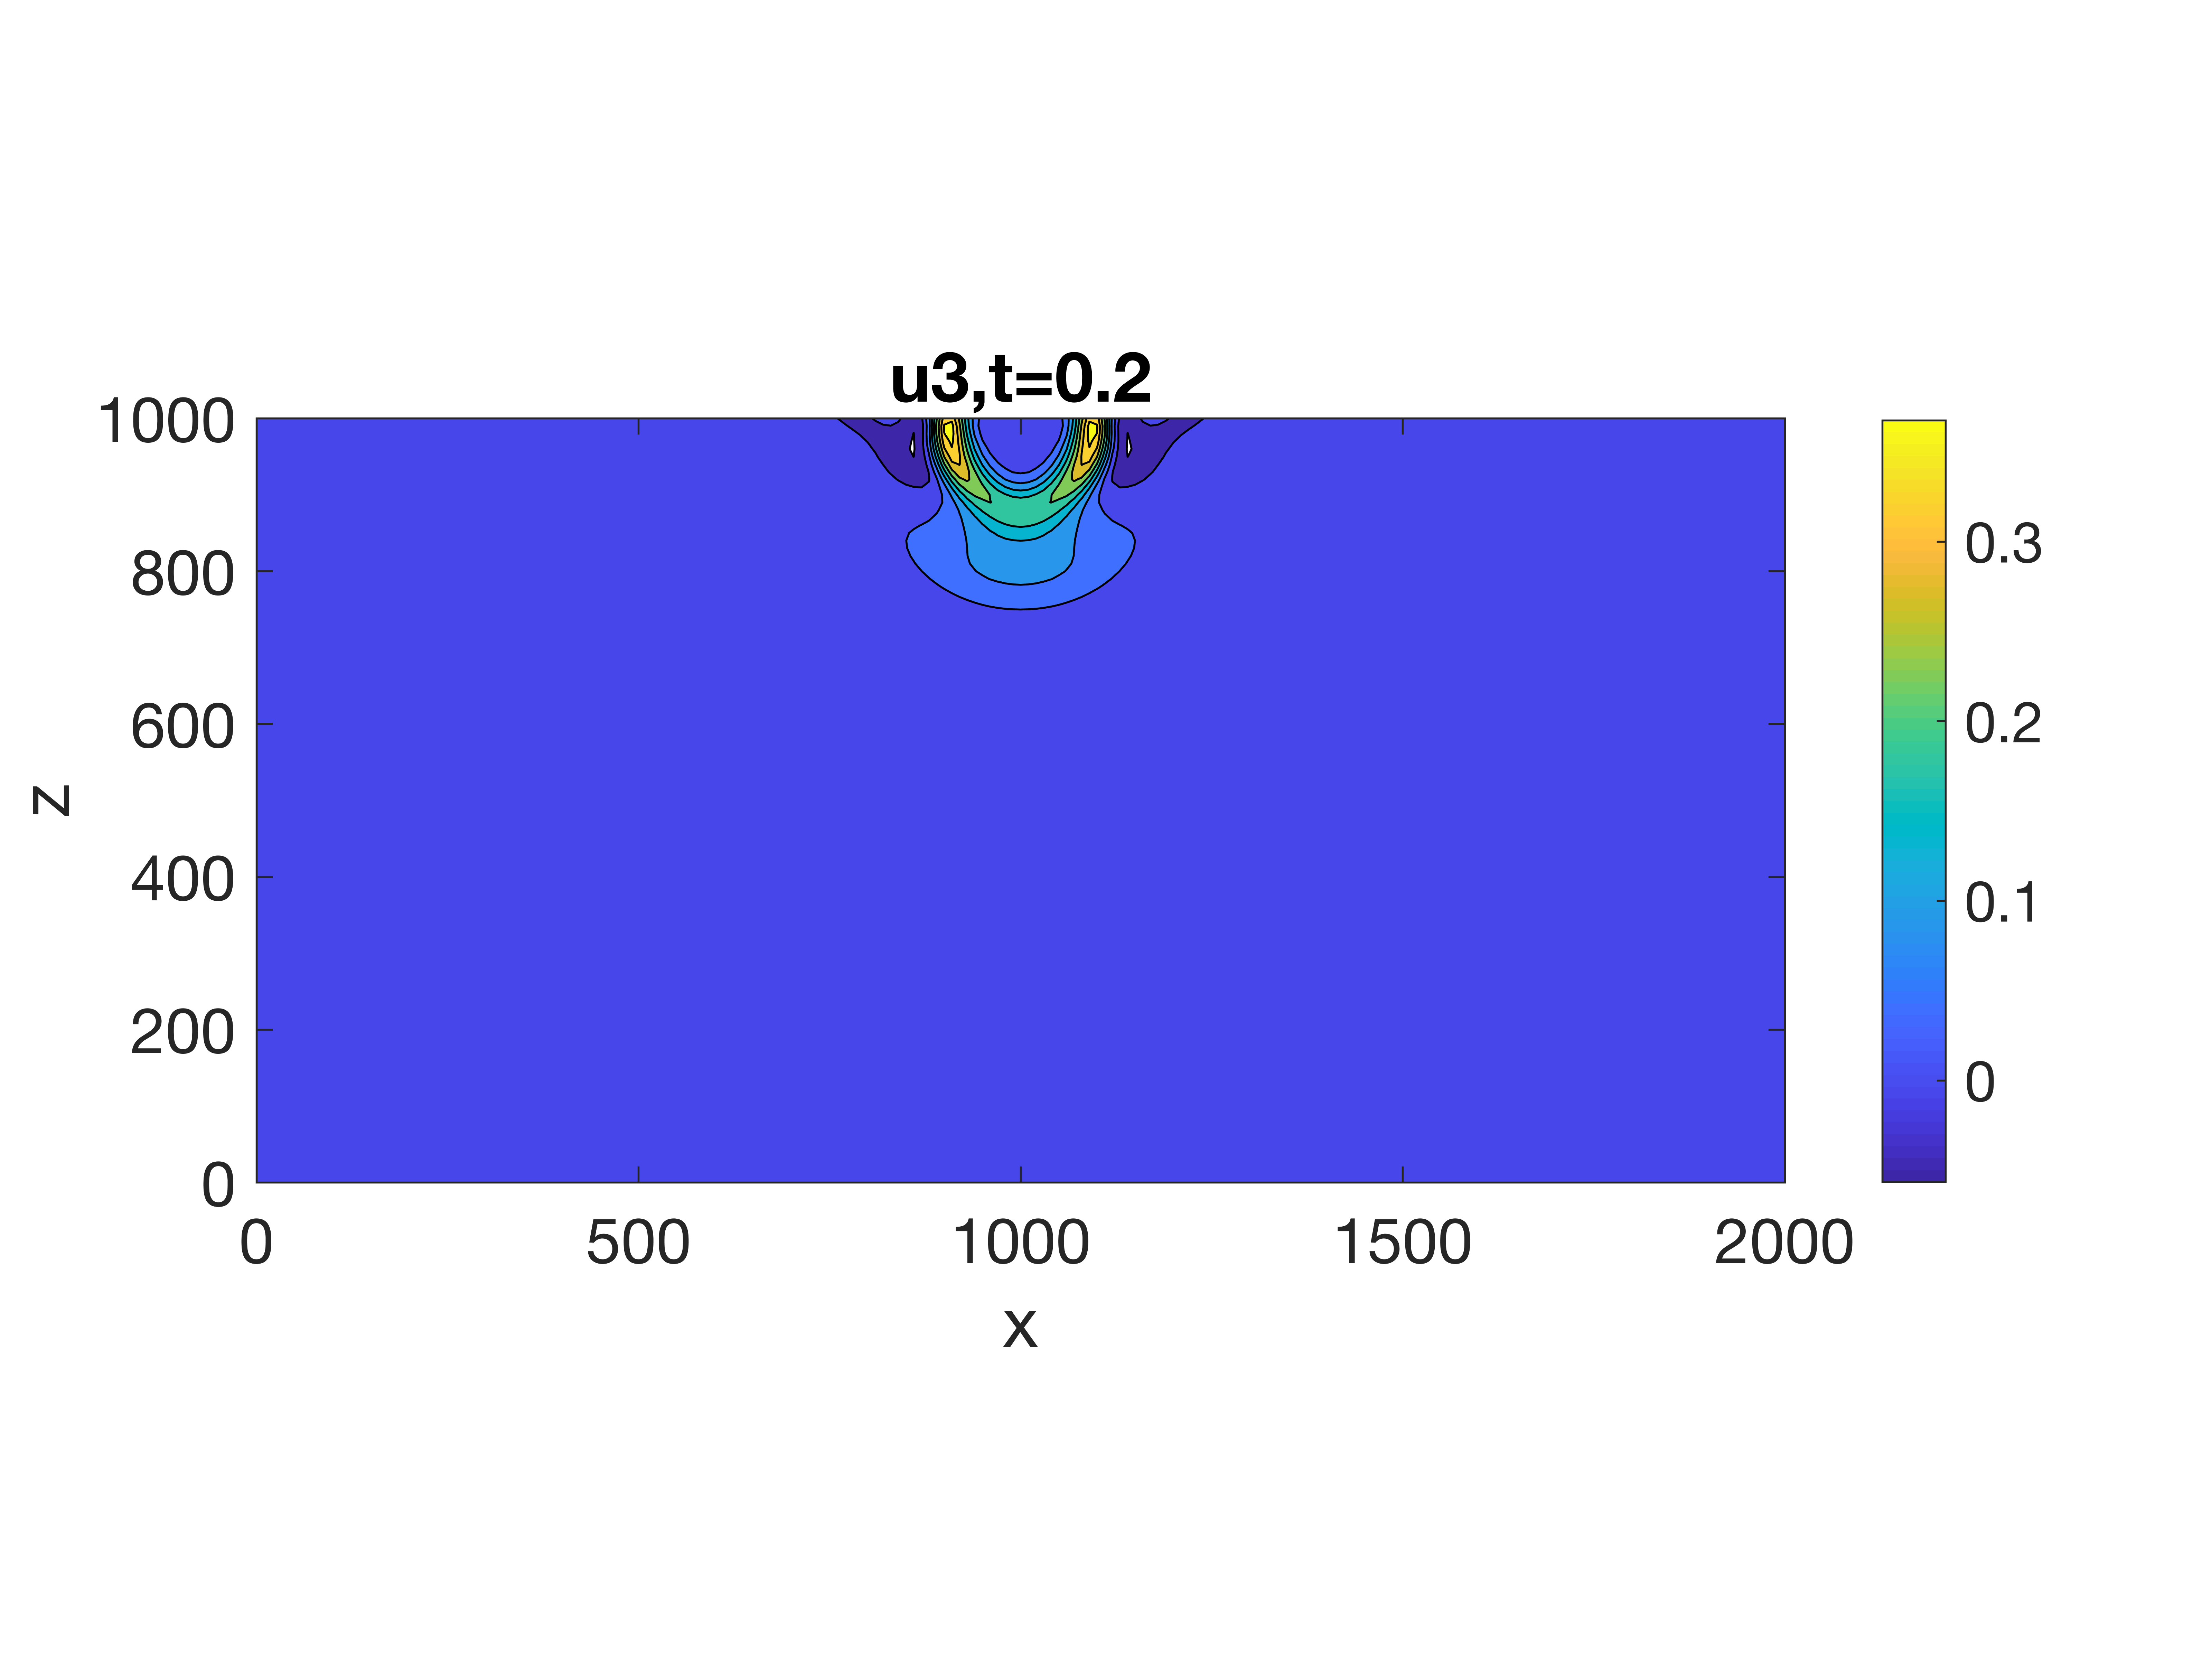
\includegraphics[width=0.4\textwidth,trim={0 2.8cm 0 2.8cm}, clip]{u3_t02_cartesian.png}
	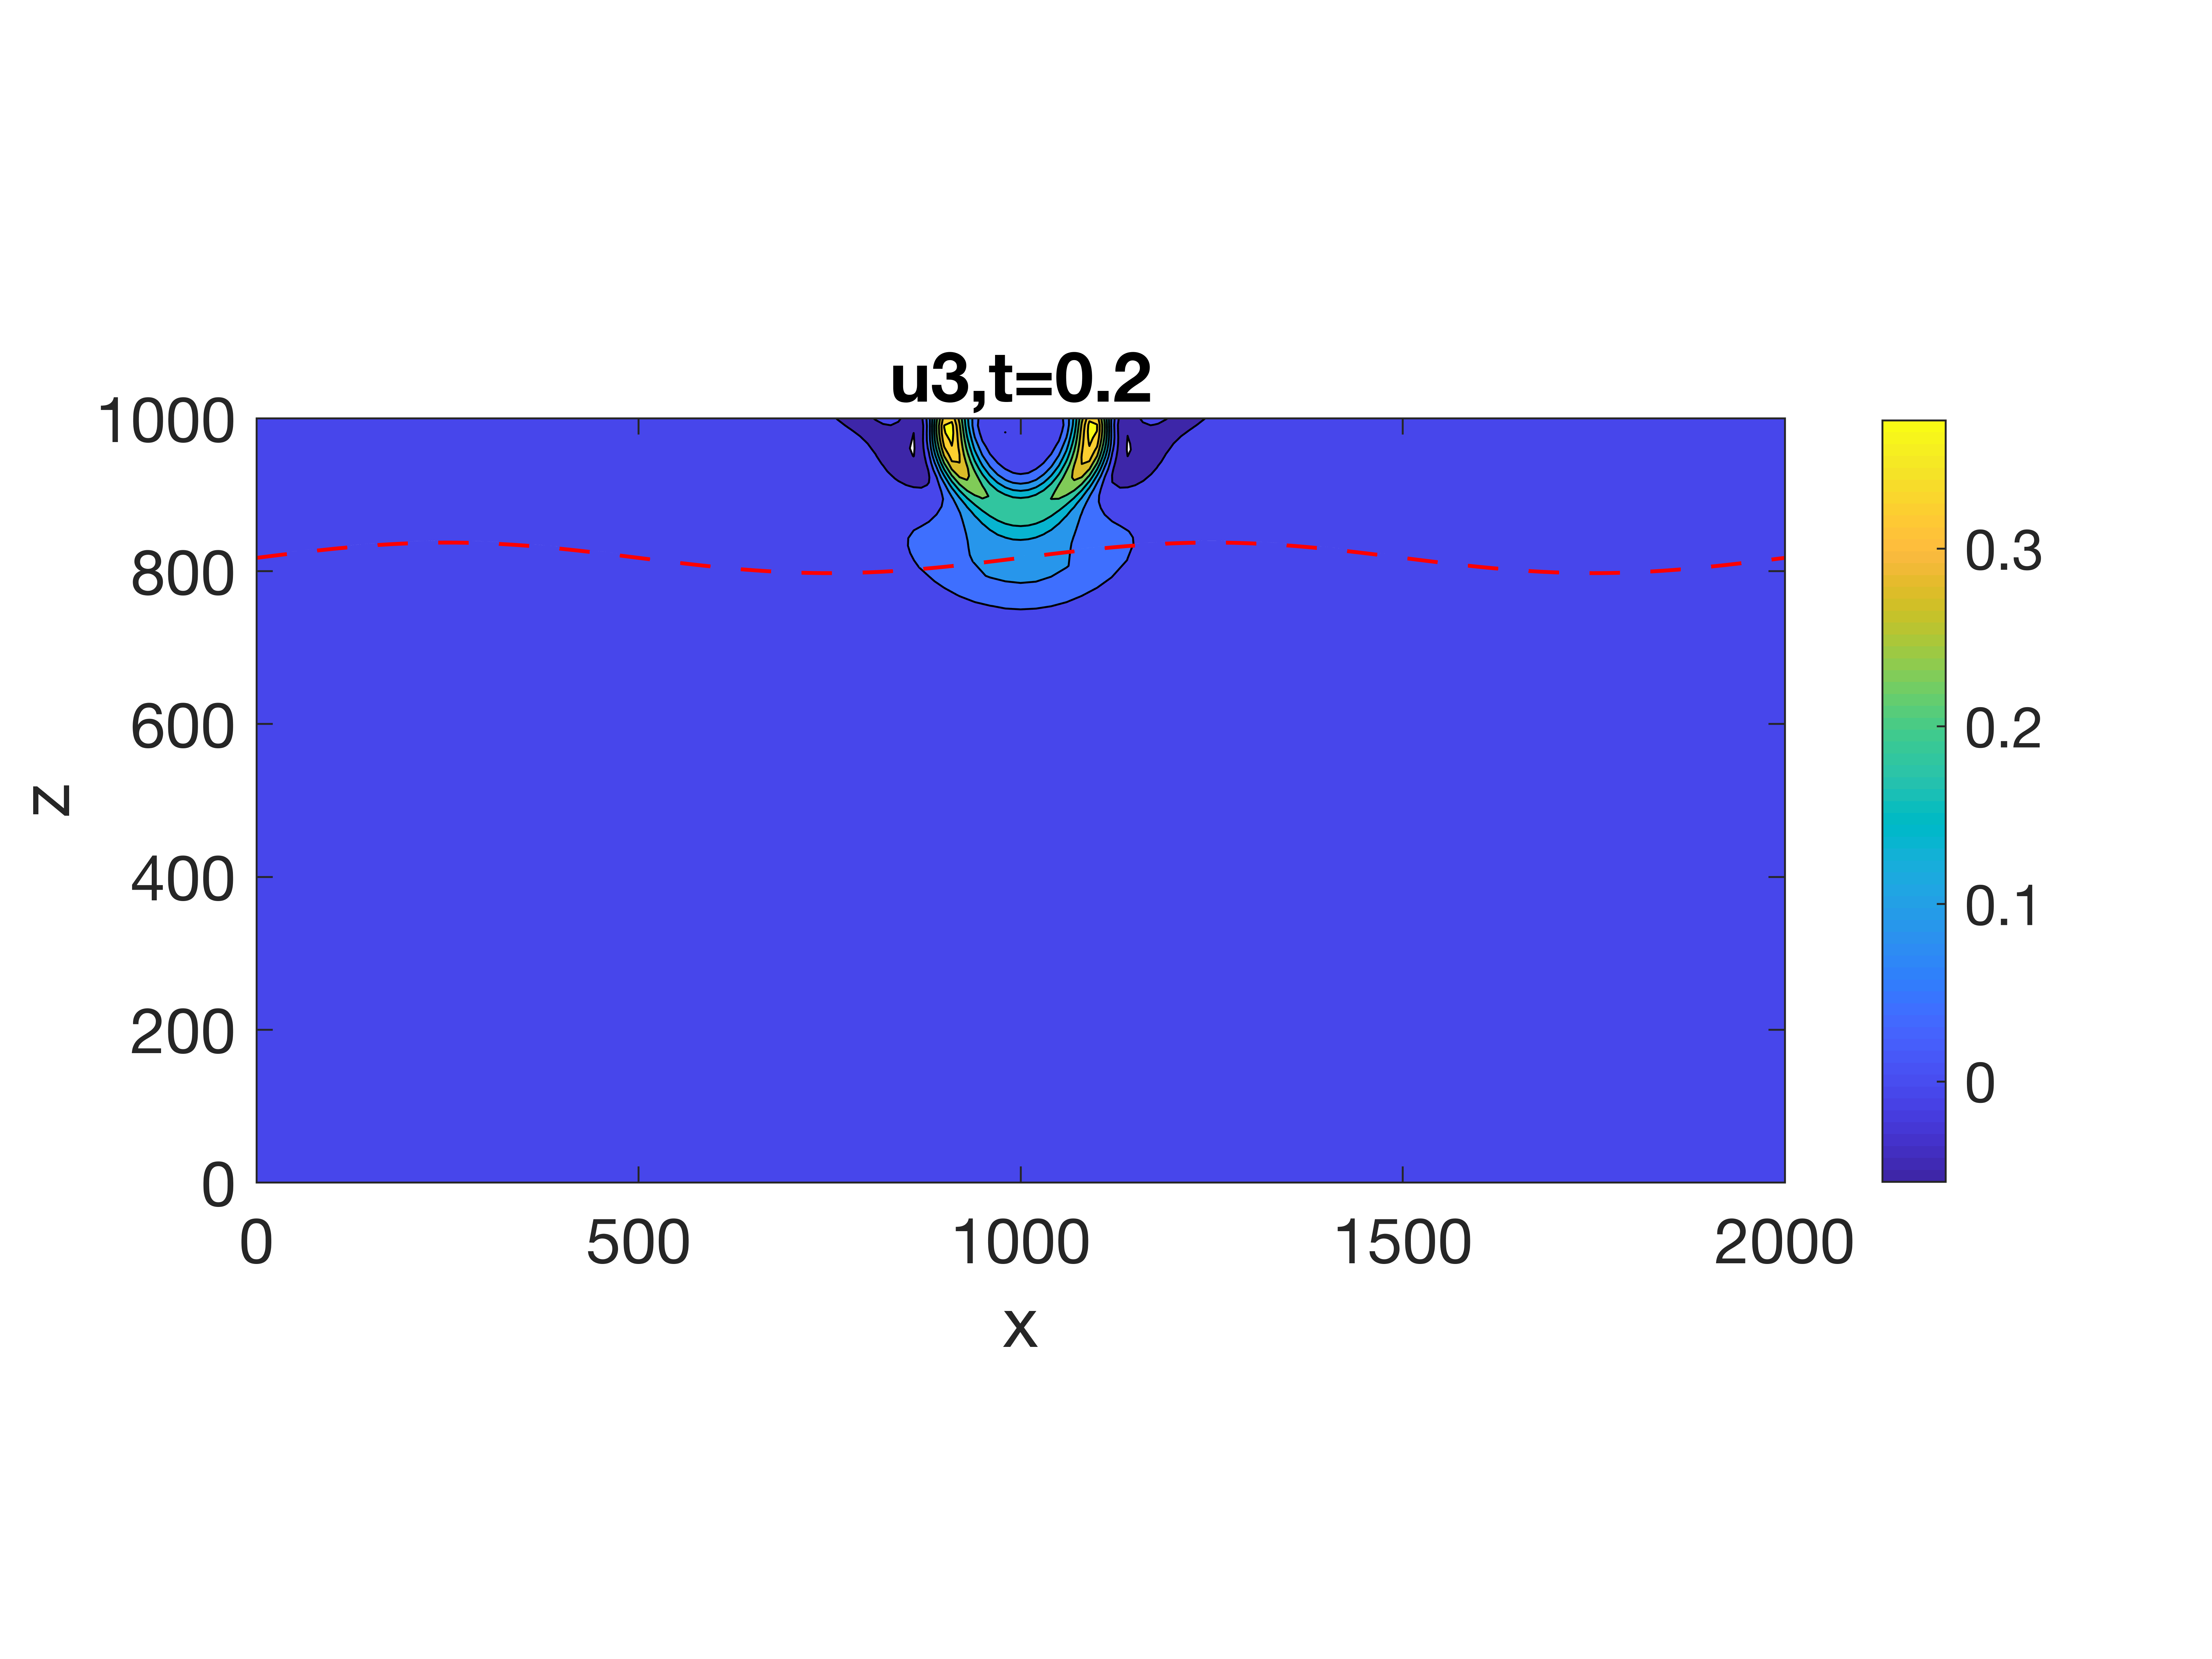
\includegraphics[width=0.4\textwidth,trim={0 2.8cm 0 2.8cm}, clip]{u3_t02_curvi_mr.png}\\
	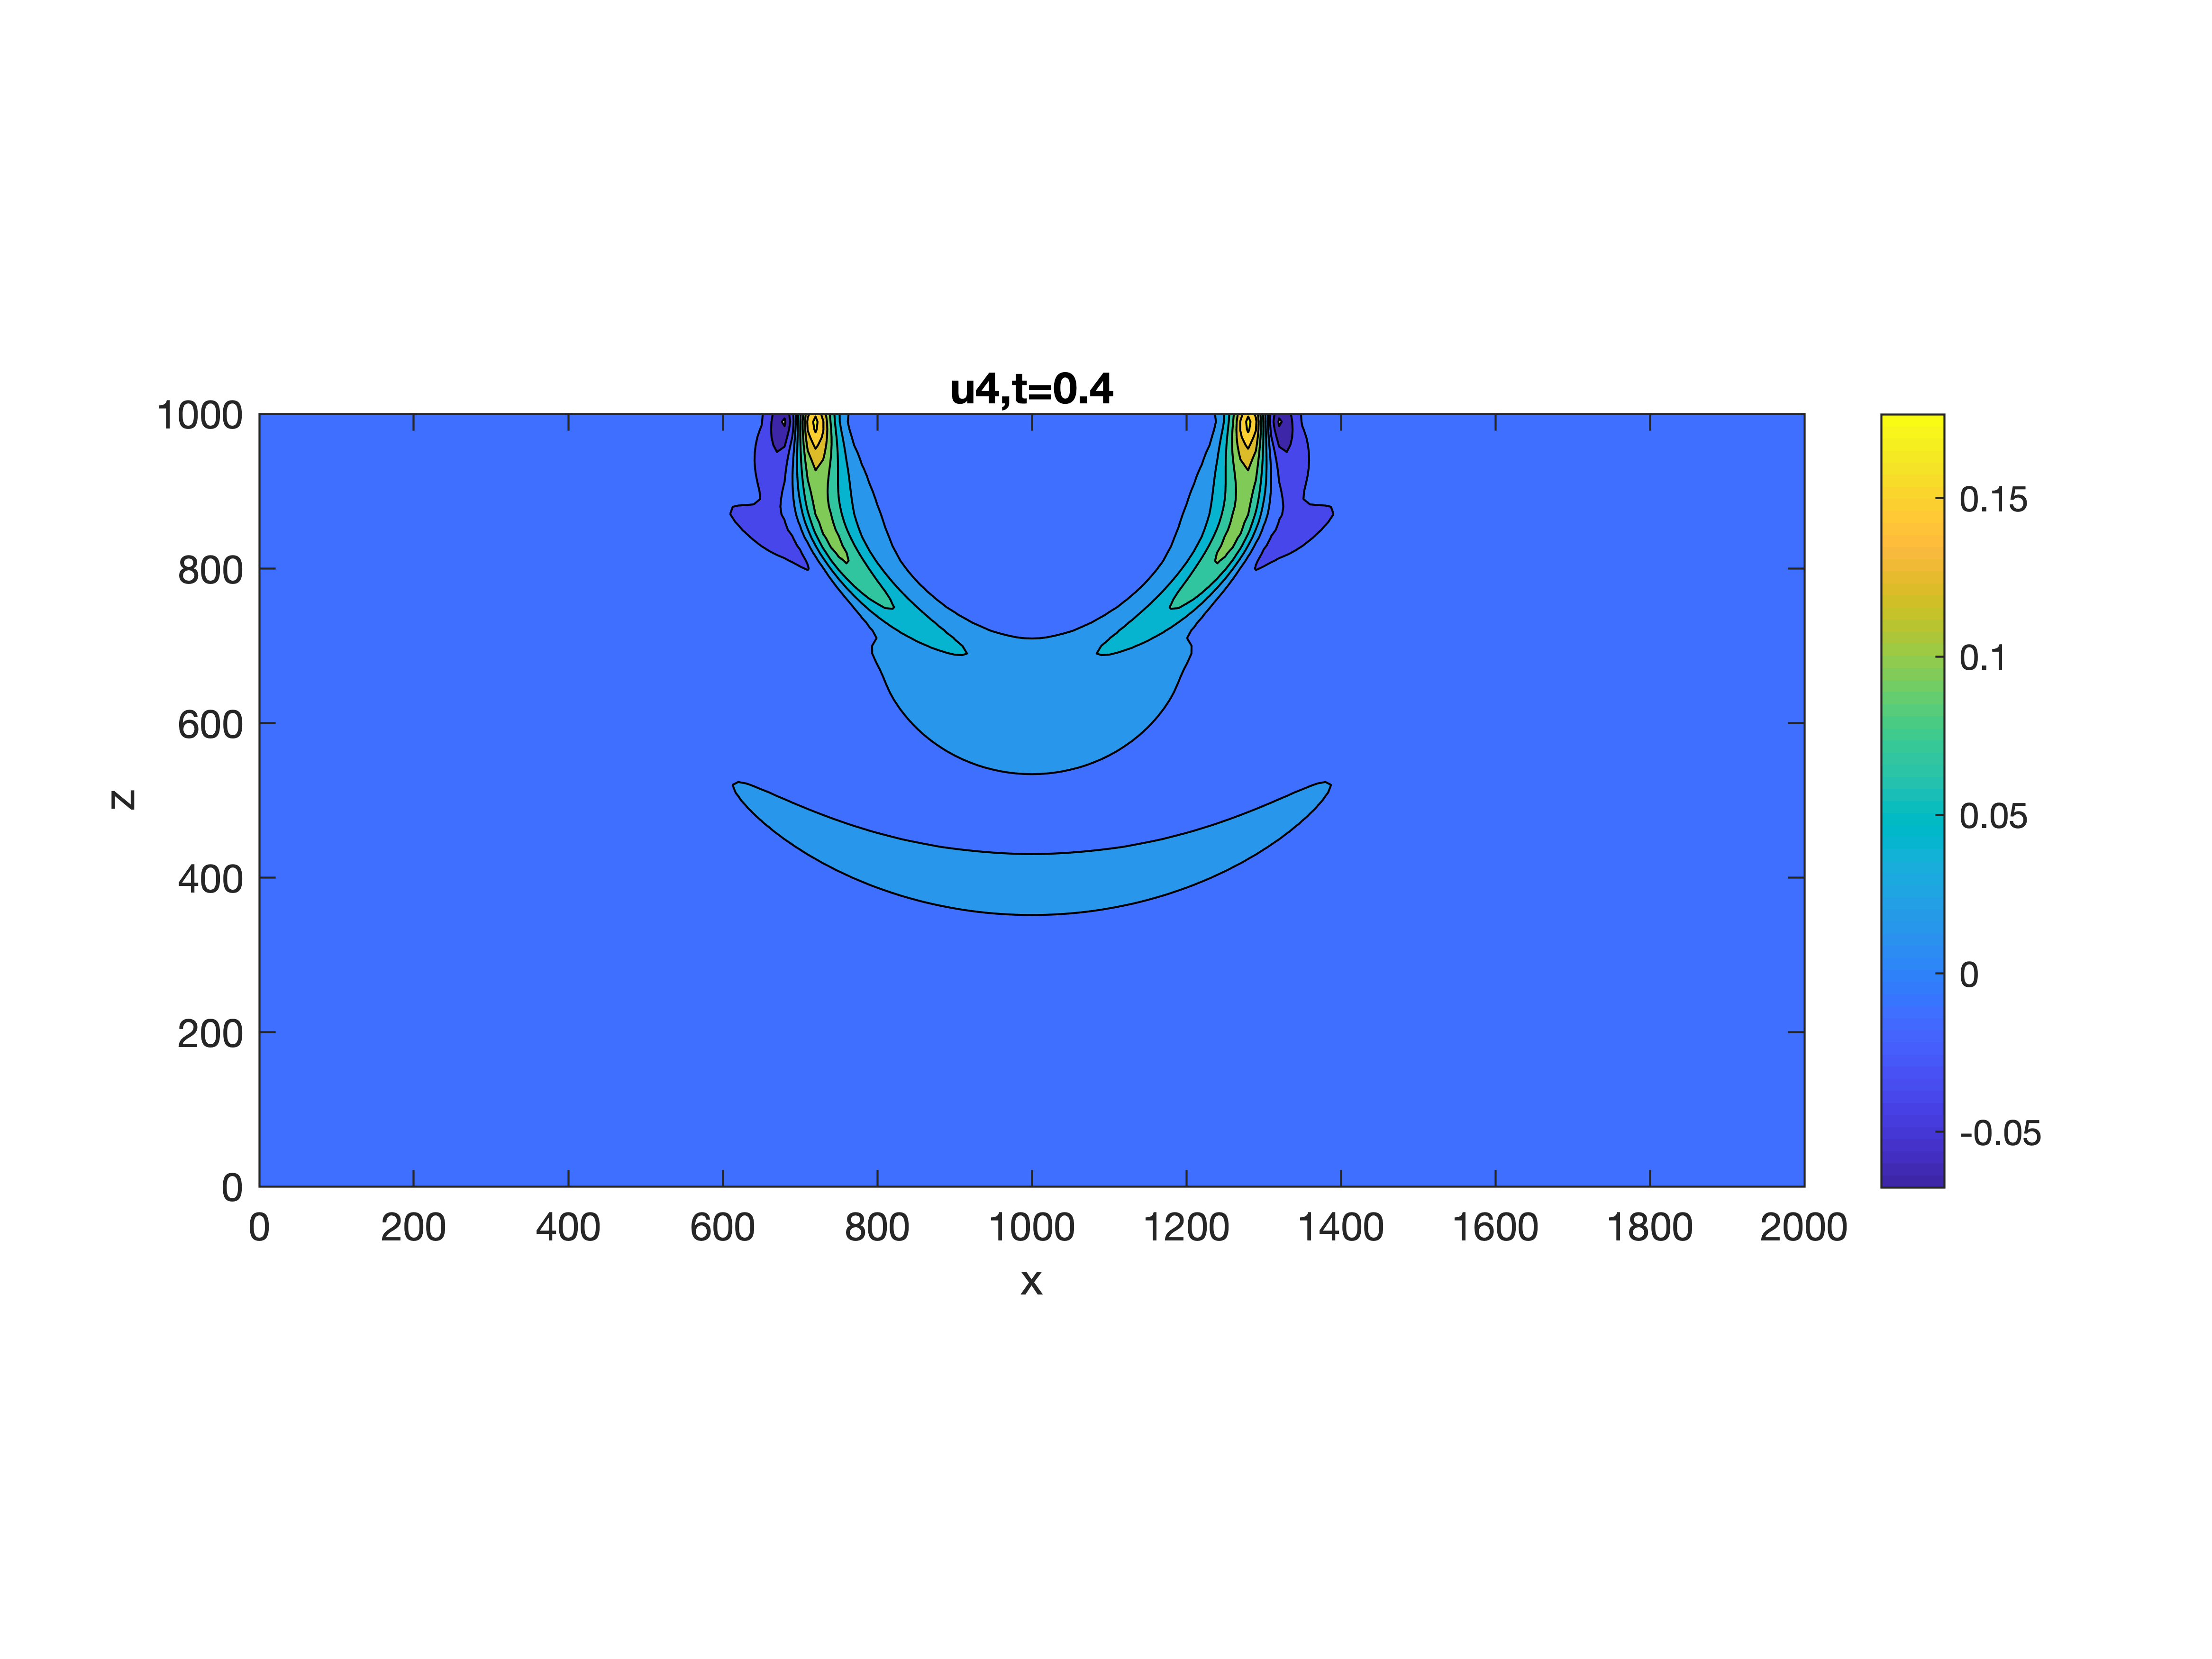
\includegraphics[width=0.4\textwidth,trim={0 2.8cm 0 2.8cm}, clip]{u3_t04_cartesian.png}
	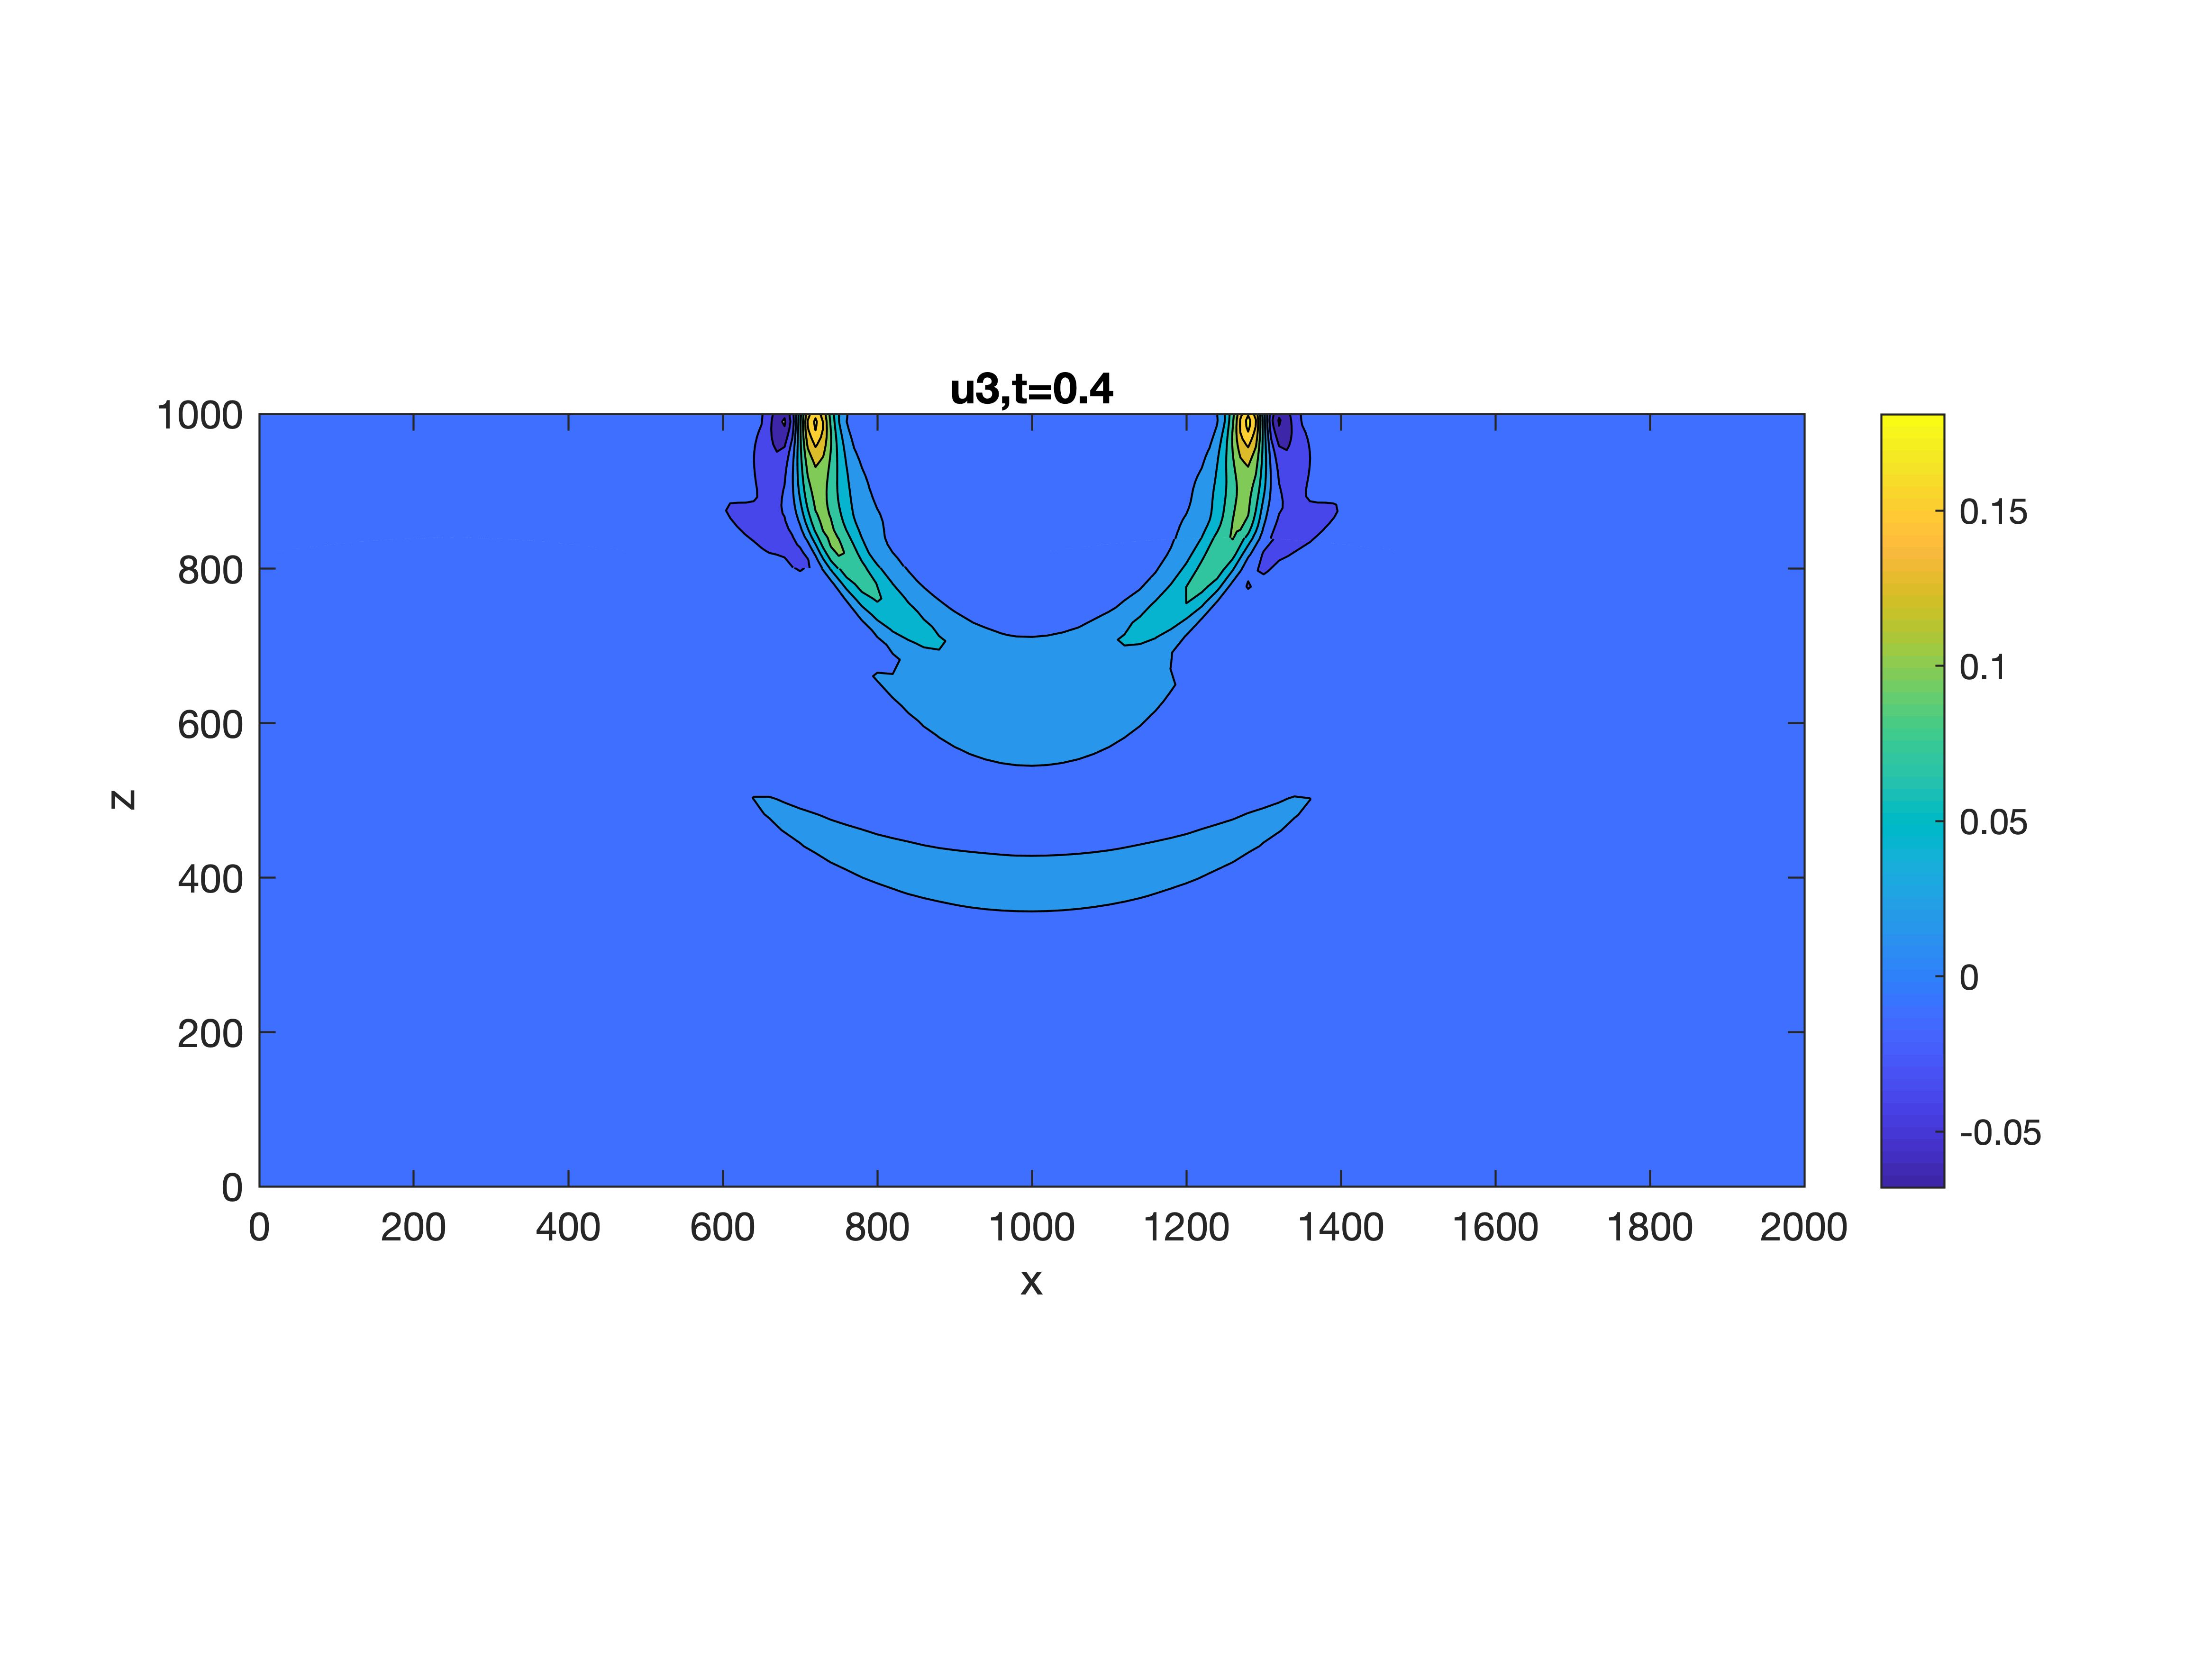
\includegraphics[width=0.4\textwidth,trim={0 2.8cm 0 2.8cm}, clip]{u3_t04_curvi_mr.png}
	\caption{The graphs for $u_3$. In the two figures on the left, we show reference solutions at $t=0.2$ and $t=0.4$, computed on a Cartesian mesh without mesh refinement interface. On the right, the two figures show the solutions computed on a curvilinear mesh with a curved mesh refinement interface at $t=0.2$ and $t=0.4$. The curved interfaces are marked with the red dash lines. Note that $x,z$ in the graph correspond to $x^{(1)}, x^{(3)}$ respectively.}
\label{u3}
\end{figure}
From Figure \ref{u1} and Figure \ref{u3}, we observe that there is no significant reflection at the mesh refinement interface for both component $u_1$ and $u_3$. As for component $u_2$, it is zero up to round-off error, and is not presented here.

%!TEX root = elastic_3d_sbp.tex
\subsection{Energy conservation test}\label{conserved_energy}
We shall have an experiment for energy conservation. We also need to evaluate the iterative methods. These can be Experiment 3, or incoporated in the first two experiments.

%!TEX root = SISC_elastic_3d.tex
\section{Conclusion}
We have developed a fourth order accurate finite difference method for the 3D elastic wave equations in heterogeneous media. To take into account discontinuous material property, we partition the domain into mesh blocks such that interfaces are aligned with material discontinuities, and the material property is smooth in each mesh block. Adjacent mesh blocks are coupled through physical interface conditions. More precisely, we impose continuity of displacements and continuity of traction. 

In a realistic setting, these mesh blocks have curved sides. We use a coordinate transformation and discretize the governing equations on curvilinear meshes. In addition, we allow nonconforming mesh refinement interfaces such that the mesh sizes in each block need not to be the same. With this important feature, we can choose the mesh size according to the velocity structure of the material, and keep the grid-point-per-wavelength almost the same in the entire domain. 

The finite difference operators satisfy a summation-by-parts property. At the interfaces, physical interface conditions are imposed by using ghost points, and mesh refinement interfaces with hanging nodes are treated numerically by fourth order interpolation operators. Together with a fourth order accurate predictor-corrector time stepping method, the fully discrete equation is energy conserving. We have conducted numerical experiments to verify the energy conserving property, and the fourth order convergence rate. Furthermore, our numerical experiments indicate that there are very little artificial reflections at the interfaces.

To obtain values on the ghost points, a system of linear equations must be solved. In our formulation, we only use ghost points from the coarse domain, and is more efficient than the traditional approach of using ghost points from both domains.  For large-scale simulations in 3D, the LU factorization cannot be used due to memory limitations. We have studied and compared three iterative methods for solving the linear system.

Currently, we are incorporating the programming code into the free software SW4 \cite{SW4}, and will test with benchmark problems on parallel machines. 

\appendix

%!TEX root = SISC_elastic_3d.tex
\section{Terms in the spatial discretization}\label{appendix_cdomain}
For the first term in (\ref{L_operator}), we have
\begin{align*}\label{3_8_1}
{Q}_l^{2h}({N}_{ll}^{2h}){\bf c} := \left(\begin{array}{c}
({Q}_l^{2h}({N}_{ll}^{2h}){\bf c})_1 \\
({Q}_l^{2h}({N}_{ll}^{2h}){\bf c})_2 \\
({Q}_l^{2h}({N}_{ll}^{2h}){\bf c})_3 
\end{array}\right), \quad ({Q}_l^{2h}({N}_{ll}^{2h}){\bf c})_p = \sum_{q = 1}^{3} Q_l^{2h}(N_{ll}^{2h}(p,q)) {c}^{(q)},\quad p = 1,2,3,
\end{align*}
where we have used a matlab notation $N_{ll}^{2h}(p,q)$ to represent the $p$-th row and $q$-th column of the matrix $N_{ll}^{2h}$; $Q_l^{2h}(N_{ll}^{2h}(p,q)){ c}^{(q)}$ is the central difference operator in direction $r^{(l)}$ for spatial second derivative with variable coefficient. For the second term in (\ref{L_operator}), we have
\begin{align*}\label{3_8_2}
\wt{{G}}_3^{2h}({N}_{33}^{2h}){\bf c} := \left(\begin{array}{c}
(\wt{{G}}_3^{2h}({N}_{33}^{2h}){\bf c})_1 \\
(\wt{{G}}_3^{2h}({N}_{33}^{2h}){\bf c})_2 \\
(\wt{{G}}_3^{2h}({N}_{33}^{2h}){\bf c})_3 
\end{array}\right), \quad (\wt{{G}}_3^{2h}({N}_{33}^{2h}){\bf c})_p = \sum_{q = 1}^{3} \wt{G}_3^{2h}(N_{33}^{2h}(p,q)) {c}^{(q)},\quad p = 1,2,3,
\end{align*}
where $\wt{G}_3^{2h}(N_{33}^{2h}(p,q)) {c}^{(j)}$ is the second derivative SBP operator  defined in (\ref{sbp_2nd_1}) for direction $r^{(3)}$. For the third term in (\ref{L_operator}), we have
\begin{align*}\label{3_8_3}
{D}_l^{2h}({N}_{lm}^{2h}{D}_m^{2h}{\bf c}) := \left(\begin{array}{c}
(D^{2h}_l(N^{2h}_{lm}D_m^{2h}{\bf c}))_1 \\
(D^{2h}_l(N^{2h}_{lm}D_m^{2h}{\bf c}))_2 \\
(D^{2h}_l(N^{2h}_{lm}D_m^{2h}{\bf c}))_3 
\end{array}\right), (D^{2h}_l(N^{2h}_{lm}D_m^{2h}{\bf c}))_p = \sum_{q = 1}^{3} D^{2h}_l(N^{2h}_{lm}(p,q)D_m^{2h}{c}^{(q)}), p = 1,2,3.
\end{align*}
Here, $D_m^{2h}c^{(q)}$ is a central difference operator in direction $r^{(m)}$ for the spatial first derivative, and $D_3^{2h}c^{(q)}$ is the SBP operator defined in (\ref{first_sbp}) for direction $r^{(3)}$.

For the second term in (\ref{Lf_operator}), we have
\begin{align*}\label{3_10_2}
{{G}}_3^{h}({N}_{33}^{h}){\bf f} := \left(\begin{array}{c}
({{G}}_3^{h}({N}_{33}^{h}){\bf f})_1 \\
({{G}}_3^{h}({N}_{33}^{h}){\bf f})_2 \\
({{G}}_3^{h}({N}_{33}^{h}){\bf f})_3 
\end{array}\right), \quad ({{G}}_3^{h}({N}_{33}^{h}){\bf f})_p = \sum_{q = 1}^{3} {G}_3^{h}(N_{33}^{h}(p,q)) {f}^{(q)},\quad p = 1,2,3.
\end{align*}
Here, ${G}_3^{h}(N_{33}^{h}(p,q)) {f}^{(q)}$ is the SBP operator defined in (\ref{sbp_2nd_2}) for direction $r^{(3)}$. 

For the terms in (\ref{hatAf}), we have
\begin{align*}\label{gamma_D} 
{N}_{3l}^hD_l^h{\bf f} := \left(\begin{array}{c}
({N}_{3l}^hD_l^h{\bf f})_1 \\
({N}_{3l}^hD_l^h{\bf f})_2 \\
({N}_{3l}^hD_l^h{\bf f})_3 
\end{array}\right), \quad ({N}_{3l}^hD_l^h{\bf f})_p = \sum_{q = 1}^{3} N_{3l}^h(p,q)D_l^h{f}^{(q)},\quad l = 1,2, \quad p = 1,2,3,
\end{align*}
where $D_l^h{f}^{(q)}$ is a central difference operator for first spatial derivative in direction $r^{(l)}$, and
\begin{align*}\label{gamma_D1}
{N}_{33}^h\mathcal{D}_3^h{\bf f} := \left(\begin{array}{c}
({N}_{33}^h\mathcal{D}_3^h{\bf f})_1 \\
({N}_{33}^h\mathcal{D}_3^h{\bf f})_2 \\
({N}_{33}^h\mathcal{D}_3^h{\bf f})_3 
\end{array}\right), \quad ({N}_{33}^h\mathcal{D}_3^h{\bf f})_p = \sum_{q = 1}^{3} N_{33}^h(p,q)\mathcal{D}_3^h{f}^{(q)},\quad p = 1,2,3,
\end{align*}
where $\mathcal{D}_3^h{f}^{(q)}$ is the SBP operator for first spatial derivative in direction $r^{(3)}$ defined as in the first equation of (\ref{sbp_1st_2}).

For the terms in (\ref{hatAc}), we have
\begin{align*}\label{3_17}
{N}_{33}^{2h}\wt{\mathcal{D}}_3^{2h}{\bf c} := \left(\begin{array}{c}
({N}_{33}^{2h}\wt{\mathcal{D}}_3^{2h}{\bf c})_1 \\
({N}_{33}^{2h}\wt{\mathcal{D}}_3^{2h}{\bf c})_2 \\
({N}_{33}^{2h}\wt{\mathcal{D}}_3^{2h}{\bf c})_3 
\end{array}\right), \quad ({N}_{33}^{2h}\wt{\mathcal{D}}_3^{2h}{\bf c})_p = \sum_{q = 1}^{3} N_{33}^{2h}(p,q)\wt{\mathcal{D}}_3^{2h}{c}^{(q)},\quad p = 1,2,3,
\end{align*}
where $\wt{\mathcal{D}}_3^{2h}{c}^{(q)}$ is the difference operator for first spatial derivative in direction $r^{(3)}$ defined as in the second equation of (\ref{sbp_1st_1}).

The term $\mathcal{S}_{2h}({\bf c}_t,{\bf c})$ in \eqref{coarse_simple} is given by
\begin{multline*}
\mathcal{S}_{2h}({\bf c}_t,{\bf c}) = ({D}_1^{2h}{\bf c}_t,{N}_{11}^{2h}{D}_1^{2h}{\bf c})_{2h} +  ({D}_1^{2h}{\bf c}_t,{N}_{12}^{2h}{D}_2^{2h}{\bf c})_{2h} +  ({D}_1^{2h}{\bf c}_t,{N}_{13}^{2h}{D}_3^{2h}{\bf c})_{2h}\\
+  ({D}_2^{2h}{\bf c}_t,{N}_{21}^{2h}{D}_1^{2h}{\bf c})_{2h} 
+  ({D}_2^{2h}{\bf c}_t,{N}_{22}^{2h}{D}_2^{2h}{\bf c})_{2h} +  ({D}_2^{2h}{\bf c}_t,{N}_{23}^{2h}{D}_3^{2h}{\bf c})_{2h} \\
+  ({D}_3^{2h}{\bf c}_t,{N}_{31}^{2h}{D}_1^{2h}{\bf c})_{2h} 
+  ({D}_3^{2h}{\bf c}_t,{N}_{32}^{2h}{D}_2^{2h}{\bf c})_{2h} +  ({D}_3^{2h}{\bf c}_t,{N}_{33}^{2h}{D}_3^{2h}{\bf c})_{2h}\\
+ ({\bf c}_t, P^{2h}_1(N_{11}^{2h}){\bf c})_{2hr} + ({\bf c}_t, P^{2h}_2(N_{22}^{2h}){\bf c})_{2hr} + ({\bf c}_t, P^{2h}_3(N_{33}^{2h}){\bf c})_{2hr},
\end{multline*}
where $P_3^{2h}(N_{33}^{2h})$ is a positive semi-definite operator defined in \eqref{sbp_2nd_1} for direction $r^{(3)}$; $P_1^{2h}(N_{11}^{2h}), P_2^{2h}(N_{22}^{2h})$ are analogue to $P_3^{2h}(N_{33}^{2h})$. 

The term $\mathcal{S}_{h}({\bf f}_t,{\bf f})$ is defined as
\begin{multline*}
\mathcal{S}_{h}({\bf f}_t,{\bf f}) = ({D}_1^{h}{\bf f}_t,{N}_{11}^{h}{D}_1^h{\bf f})_{h} +  ({D}_1^{h}{\bf f}_t,{N}_{12}^{h}{D}_2^h{\bf f})_{h} +  ({D}_1^{h}{\bf f}_t,{N}_{13}^{h}{D}_3^h{\bf f})_{h}\\
+  ({D}_2^{h}{\bf f}_t,{N}_{21}^{h}{D}_1^h{\bf f})_{h} 
+  ({D}_2^{h}{\bf f}_t,{N}_{22}^{h}{D}_2^h{\bf f})_{h} +  ({D}_2^{h}{\bf f}_t,{N}_{23}^{h}{D}_3^h{\bf f})_{h} \\
+  ({D}_3^{h}{\bf f}_t,{N}_{31}^{h}{D}_1^h{\bf f})_{h} 
+  ({D}_3^{h}{\bf f}_t,{N}_{32}^{h}{D}_2^h{\bf f})_{h} +  ({D}_3^{h}{\bf f}_t,{N}_{33}^{h}{D}_3^h{\bf f})_{h}\\
+ ({\bf f}_t, P^{h}_1(N_{11}^h){\bf f})_{hr} + ({\bf f}_t, P^{h}_2(N_{22}^h){\bf f})_{hr} + ({\bf f}_t, P^{h}_3(N_{33}^h){\bf f})_{hr}.
\end{multline*}
Here, $P_l^h(N_{ll}^h)$ are defined similar as $P_l^{2h}(N_{ll}^{2h})$ in $\mathcal{S}_{2h}({\bf c}_t,{\bf c})$. 


\bibliography{lu}
\bibliographystyle{siamplain}


\end{document}
